%
% platex SpMCvx.tex
% jbibtex [each included files]
% platex again
%
%\documentclass[a4paper,12pt,oneside]{jbook}
\documentclass[a4paper,12pt]{jbook}

% my own definitions
\usepackage{mytext}
\usepackage{mydef}


\newcommand{\chapmark}{}
% 番号なしの見出し
\newcommand{\Chapter}[1]{\chapter*{#1}
\renewcommand{\chapmark}{#1}
\addcontentsline{toc}{chapter}{\prechaptername #1}}
\newcommand{\Section}[1]{\section*{#1}
\addcontentsline{toc}{section}{#1}}
\newcommand{\Subsection}[1]{\subsection*{#1}
\addcontentsline{toc}{subsection}{#1}}
\newcommand{\Subsubsection}[1]{\subsubsection*{#1}
\addcontentsline{toc}{subsubsubsection}{#1}}

% chapter毎に参考文献
\usepackage{chapterbib}

% include figures
\usepackage[dvipdfmx]{color}
\usepackage[dvipdfmx]{graphicx}
\usepackage{mediabb}

% math symbols, theorems
\usepackage{amssymb}
\usepackage{amsthm}

% header and footer
\usepackage{fancyhdr}

% box enclosure
%\usepackage{eclbkbox}
\usepackage{listings,jlisting}

%\usepackage{lastpage}

% force to put figure here
\usepackage{here}

% strikeout
\usepackage{ulem}

% date
\usepackage{datetime}
\newcommand{\numtoday}{\the\year\twodigit\month\twodigit\day}


%\iffalse
\usepackage{algorithm}
\usepackage{algorithmic}
% アルゴリズム環境の設定 (using algorithmic and algorithm)
\floatname{algorithm}{アルゴリズム}
\renewcommand{\algorithmicrequire}{\textbf{入力:}}
\renewcommand{\algorithmicensure}{\textbf{出力:}}
\algsetup{linenosize=\normalsize,linenodelimiter=\ }
\renewcommand{\algorithmiccomment}[1]{// #1}
%\fi


%\lhead{情報システム論II}
%\chead{上の真ん中}
%\rhead{\rightmark}
%\rfoot{Ver. \numtoday}
%\rfoot{\copyright 2015 Tomoya Sakai}
%\rfoot{\ifthenelse{\value{page}=\pageref{LastPage}}{(to be continued ...)}{}}
\fancyfoot[RO]{\copyright 2015 Tomoya Sakai}
\fancyfoot[C]{}
\fancyhead[RO,LE]{\thepage}
\fancyhead[RE]{酒井研 基礎勉強会}
\fancyhead[LO]{\chapmark}



% 数式定義
\def\ds{\displaystyle}
\def\refeq#1{(\ref{eq:#1})}
\def\vec#1{\mbox{\boldmath $#1$}}
%\def\vec#1{{\rm\bf #1}}
\def\mtr#1{\mbox{\boldmath $#1$}}
%\def\mtr#1{{\rm\bf #1}}
\def\tten#1{{\!\times\!10^{#1}}}
\def\defas{:=}
\def\subs{:=}
\def\smatrix#1#2#3{\mbox{#1$\bmatrix{#2}{#3}$}}
\def\spark{\mathop{\textrm{spark}}\nolimits}
\def\soft{\mathop{\textrm{soft}}\nolimits}
\def\prox{\mathop{\textrm{prox}}\nolimits}


%% MATLAB code
\lstset{language=Matlab}
\lstset{basicstyle={\tt},identifierstyle={\bfseries},keywordstyle={\bfseries}}
\lstset{tabsize=2,showstringspaces=false}
\lstset{commentstyle={\color[rgb]{0,0.5,0}}}
\lstset{flexiblecolumns=true}
\lstset{classoffset=1,breaklines=true,morecomment=[l]{//}}
%\lstset{columns=[l]{fullflexible}}
%\lstset{numbers=left,stepnumber=1,numberstyle={\scriptsize},numbersep=4ex}
\lstset{frame=tBlR,rulecolor={\color[gray]{0.75}},rulesepcolor={\color[gray]{0.75}}}
\lstset{framesep=2ex}
\lstset{xleftmargin=8ex,xrightmargin=16ex}
%\lstset{backgroundcolor={\color[rgb]{1,1,0.95}}}

\def\yeeks{${\!\!\!\!^*\;\;}$}


% link url
\AtBeginDvi{\special{pdf:tounicode 90ms-RKSJ-UCS2}}
\usepackage[bookmarks=false,urlcolor=blue,colorlinks,linkcolor=blue,dvipdfmx,%
%pdftitle={},
pdfauthor={Tomoya Sakai}%
]{hyperref}



\begin{document}
\pagenumbering{arabic}

\pagestyle{empty}

\vspace*{6cm}
%% タイトル直書き・・
\begin{center}
{%\spaceskip=0.25em
\Large\bf 酒井研 基礎勉強会 テキスト}\\
{\bf スパースモデリングと凸最適化}\\
\vspace{2\baselineskip}
酒井智弥\\
\today
\end{center}

\pagestyle{empty}
\tableofcontents

\pagestyle{fancy}

\Chapter{準備}




\Section{ベクトル・行列に関する表記法}
\label{sec:notation}

ベクトルや行列について本書が好んで用いる表記法を紹介する.


\paragraph{スカラーとベクトル}
本書では,実数の集合を$\mathbb{R}$と表す.
例えば,$x\in\mathbb{R}$という記述は,
「$x$は実数のスカラー(scalar)である」という意味である.
また,2つの実数の組の集合を直積で表し,
$\mathbb{R}\times\mathbb{R}=\mathbb{R}^2$と記す.
例えば,$\vec x\in\mathbb{R}^2$は,
$\vec x$が2つの実数の組で表される量であることを意味する.
本書では,これを単に「$\vec x$は2次元のベクトル(vector)である」と言う.
同様に,$\vec x\in\mathbb{R}^d$(ただし$d$は正の整数)という記述は,
「$\vec x$は$d$次元ベクトルである」という意味である.

\paragraph{空間}
%$\mathbb{R}^d$は単に$d$個の実数の組に過ぎないが,
%これを「$d$次元空間」と呼ぶことがある.
空間(space)には,その性質や構造を備えるために内積や距離などが定義されている.
例えば,実ベクトル空間は線形演算が定義された実数の配列の集合である.
% set of arrays of real numbers with linear operations
$\mathbb{R}^d$は単に$d$個の実数からなる配列の全体集合に過ぎないが,
特に明示しない場合でも何らかの演算が定義されていることを意図して,
本書では$\mathbb{R}^d$を「$d$次元空間」と単に呼ぶことがある.
ただし,必ずしもお馴染みのユークリッド距離が定義されているユークリッド空間では
ないかもしれないので注意されたい.

\paragraph{行列}
$m$行$n$列の実数の配列で表される量を実行列(real matrix)と呼び,
その全体集合を$\mathbb{R}^{m\times n}$と表す.
例えば,$\mtr A\in\mathbb{R}^{m\times n}$は,
「$\mtr A$はサイズが$m\times n$の行列である」という意味である.
ふたつの集合$[m]=\{1,\dots,m\}$と$[n]=\{1,\dots,n\}$の
直積$[m]\times[n]=\{(1,1),(1,2),\dots,(m,n)\}$を添え字の集合とすると,
行列は添え字から実数への対応付け$[m]\times[n]\rightarrow\mathbb{R}$を
表していると見なせる.
その略記が$\mathbb{R}^{m\times n}$の由来と考えられる.
なお,本書では行列$\mtr A\in\mathbb{R}^{m\times n}$の
第$ij$要素を$a_{ij}$と表記することがある.
また,第$j$列を$\vec a^{(j)}\in\mathbb{R}^m$と書き表す.
\[
 \mtr A=\left[\vec a^{(1)}\;\vec a^{(2)}\;\cdots\;\vec a^{(n)}\right]\;\in\;\mathbb{R}^{m\times n}
\]


\paragraph{転置}
行列$\mtr A\in\mathbb{R}^{m\times n}$の行と列の添え字を入れ替えた行列を
$\mtr A^\top\in\mathbb{R}^{n\times m}$と記す
\footnote{文献によっては$\mtr A^T$,${}^t\mtr A$,$\mtr A'$などと記されることもある.}.
これは行列の転置(transposition)と呼ばれる操作であり,$\top$は転置の演算子である.\\
例:
\[
\mtr A=\bmatrix{cc}{1.1 & 1.2\\ 2.1 & 2.2\\ 3.1 & 3.2}\in\mathbb{R}^{3\times 2}
\qquad\Leftrightarrow\qquad
\mtr A^\top=\bmatrix{ccc}{1.1 & 2.1 & 3.1\\ 1.2 & 2.2 & 3.2}\in\mathbb{R}^{2\times 3}
\]
この例のように,本書では行列の要素を並べた配列を大括弧で括って記述する.
%
また,複素数を要素とする行列$\mtr A\in\mathbb{C}^{m\times n}$に対して,
転置行列の複素共役を随伴行列,エルミート転置行列などと呼び,
$\mtr A^\dagger$や$\mtr A^H$などと書き表す.


\paragraph{ベクトルの成分}
サイズ$d\times 1$の行列は$d$次元の列ベクトルと呼ばれ,
サイズ$1\times d$の行列は$d$次元の行ベクトルと呼ばれる.
本書で$\vec x\in\mathbb{R}^d$と記したときは,
特に断りがない場合,$\vec x$は列ベクトルであるものとする.
なお,$d$個の実数$x_1,x_2,\dots,x_d$を成分にもつ
列ベクトル$\vec x\in\mathbb{R}^d$を,
紙面の都合上,$\vec x=[x_1,\dots,x_d]^\top$と書き表すことがある.\\
例:
\[
\vec x=\bmatrix{c}{1.1\\ 2.1\\ 3.1\\ 4.1}\in\mathbb{R}^4
\quad\Leftrightarrow\quad
\vec x=[1.1,\,2.1,\,3.1,\,4.1]^\top
\quad\Leftrightarrow\quad
\vec x^\top=[1.1\,,2.1\,,3.1\,,4.1]
\]


\paragraph{内積}
%行列$\mtr A\in\mathbb{R}^{m\times c}$は,
%その列数$c$と等しい行数をもつ行列$\mtr B\in\mathbb{R}^{c\times n}$と
%掛け合わせることができる.
%それぞれの行列の第$ij$要素を$a_{ij}$,$b_{ij}$とすると,
%行列の積$\mtr C=\mtr A\mtr B\in\mathbb{m\times n}$の
%第$ij$要素は$c_{ij}=\sum{k=1}^c a_{ik}b_{kj}$である.
%
%内積は,次元数が同じ2つのベクトルからスカラーを得る演算である.
行列の乗算の規則を利用して,
次元数が同じ2つのベクトル$\vec a,\vec b\in\mathbb{R}^d$の内積を本書では
%$\vec a^\top$と$\vec b$の積
$\vec a^\top\vec b=a_1b_1+a_2b_2+\cdots+a_db_d\in\mathbb{R}$
と書き表す.
例:
\[
\vec a=[1,\,2,\,3]^\top,\;\vec b=[2,\,-3,\,4]^\top
\quad\Leftrightarrow\quad
\vec a^\top\vec b=1\cdot 2+2\cdot (-3)+3\cdot 4 = 8
\]
%なお,
%任意の次元数の2つのベクトル$\vec a\in\mathbb{R}^m$と$\vec b\in\mathbb{R}^n$の積
%$\vec a\vec b^\top\in\mathbb{R}^{m\times n}$は行列である.



\paragraph{ノルム}
ノルム(norm)は,長さ・大きさを表す非負の関数であり,
$\|\cdot\|$という記号を用いて書き表す.
本書には,何種類かのノルムが登場する.
%
最も単純な実数$x\in\mathbb{R}$に対するノルムは,
実数の大きさを表す絶対値$\|x\|=|x|$に他ならない.
%
ベクトル$\vec x\in\mathbb{R}^d$の$p$ノルムまたは$\ell_p$ノルムと呼ばれるノルムは
\[
 \|\vec x\|_p=\left(|x_1|^p+|x_2|^p+\cdots+|x_d|^p\right)^{\frac{1}{p}}
\]
と定義されている.
$p=2$のときユークリッドノルム,$p=1$のとき絶対値ノルムとも呼ばれる.
行列のノルムもいくつか定義されており,
ベクトルのノルムを行列に対して一般化したものが多い.
例えば,行列$\mtr A\in\mathbb{R}^{m\times n}$の$\ell_p$ノルムは
\[
 \|\mtr A\|_p=\left(\sum_{i=1}^m\sum_{j=1}^n|a_{ij}|^p\right)^{\frac{1}{p}}
\]
と定義される.
特に,$p=2$のときフロベニウスノルム(Frobenius norm)と呼ばれ,次式のように表記される.
\[
 \|\mtr A\|_F=\sqrt{\sum_{i=1}^m\sum_{j=1}^n|a_{ij}|^2}
\]
これとは異なる行列ノルムの定義もある.
シャッテン$p$ノルム(Schatten $p$-norm)は,
行列$\mtr A\in\mathbb{R}^{m\times n}$の
特異値(singular values)$\vec\kappa=[\kappa_1,\dots,\kappa_{\min(m,n)}]^\top$を用いて
$\|\mtr A\|_p=\|\vec\kappa\|_p$と定義された行列ノルムである.
$\mtr A$の特異値は,
正方行列$\mtr A\mtr A^\top$または$\mtr A^\top\mtr A$の固有値の平方根であり,
$\mtr A$の列ベクトルまたは行ベクトルが表すデータの分布の広がりを表す量である.
$p=2$のとき,シャッテンノルムはフロベニウスノルムと一致する.
また,$p=1$のシャッテンノルムは特異値の総和を表す.
これを核ノルム(nuclear norm)またはトレースノルム(trace norm)
\footnote{$\|\mtr A\|_*=\tr(\sqrt{\mtr A^\top\mtr A})$と書き表せることに由来する.}
と呼び,
次式のように表記する.
\[
 \|\mtr A\|_*=\sum_{k=1}^{\min(m,n)}\kappa_k
\]


\iffalse

arg min
differntiation of quadratic form etc.



%\begin{tabular}{ll}
%\end{tabular}


\Section{演習問題}
\begin{enumerate}
\item
適当に作成した$n$本のベクトルについて,
ランダム射影前後のノルムの相対誤差$\varepsilon^{(j)}$を計算せよ.
\[
  \varepsilon^{(j)}=\frac{\|\vec p^{(j)}\|-\|\vec x^{(j)}\|}{\|\vec x^{(j)}\|}\quad (j=1,\dots,n).
\]
\item
相対誤差のヒストグラムを作成し,分布を観察せよ.
ランダム射影先の次元数$d_p$が小さいと誤差はどうなるか.
いくつか異なる次元数$d_p$についてヒストグラムを作成し,観察せよ.\\
ヒント:MATLABでは,{\tt e}をベクトルとすると,
{\tt hist(e,30)}は{\tt e}の成分についてビン数30のヒストグラムを作る.
\item ランダム射影とノルム(または距離)の計算時間を測定せよ.\\
ヒント:{\tt tic; p = R *x; toc}とすると,{\tt p = R * x}の
実行にかかった時間が表示される.
\item\yeeks
計算時間とメモリ使用量がとても少ない
効率的なランダム射影のアルゴリズムがある\cite{Sakai09ERPj,tsakaiAPR11}.
そのアルゴリズムは,サイズ$d_p\times d_x$のランダム行列を生成する必要がない.
どのようなアルゴリズムなのか調べよ.
\item\yeeks
Jhonson-Lindenstraussの埋め込み\cite{JL84,Achlioptas03,Dasgupta99,Vempala04}
とは何か調査せよ.
また,ランダム射影後の2点間の距離の誤差に関する命題を見つけ,説明せよ.
\end{enumerate}
\fi


\iffalse

{\footnotesize
\bibliography{mybib_rp}
}

\section*{See also:}
{\footnotesize
\begin{description}
\item[\href{https://drive.google.com/file/d/0Bx4bEpaTSFcgOFA5dVZoZXFkRmc}{[Sakai, 09]}\cite{Sakai09ERPj}]
https://drive.google.com/file/d/0Bx4bEpaTSFcgOFA5dVZoZXFkRmc
\item[\href{https://drive.google.com/file/d/0Bx4bEpaTSFcgZWp2ZDRLa2c1SEE}{[Sakai\&Imiya,11]}\cite{tsakaiAPR11}]
https://drive.google.com/file/d/0Bx4bEpaTSFcgZWp2ZDRLa2c1SEE
\item[\href{http://vision.ucsd.edu/~leekc/ExtYaleDatabase/ExtYaleB.html}{The Extended Yale Face Database B}]
http://vision.ucsd.edu/~leekc/ExtYaleDatabase/ExtYaleB.html\\
cropped images in MATLAB file: \href{https://drive.google.com/file/d/0Bx4bEpaTSFcgRm15NVlua1pOTWM}{YaleB\_Ext\_Cropped\_192x168\_all.mat}\\
https://drive.google.com/file/d/0Bx4bEpaTSFcgRm15NVlua1pOTWM
\end{description}
}

\fi

%\bibliographystyle{ieeetr}
%\bibliographystyle{splncs}
%\bibliographystyle{elsart-harv}
%\bibliographystyle{ipsjunsrt-e}
\bibliographystyle{ieicetr}




\Chapter{かけると便利なスクランブル --- ランダム射影 ---}


\Section{原理}

ランダム射影(random projection)は,乱数で作った行列$\mtr R$による
線形写像である.
$d_x$次元ベクトル$\vec x\in\mathbb{R}^{d_x}$から
$d_p$次元ベクトル$\vec p\in\mathbb{R}^{d_p}$へのランダム射影は
\begin{equation}
%\mbox{\ RandomProjection(\vec x\|\mtr R)}\defas
\vec p=\mtr R\vec x
\end{equation}
と書ける.
$\vec x$は$d_x$次元ベクトルで,
実数の成分を持つどんなベクトルでも構わない.
$\vec p$は$d_p$次元ベクトルである.
$d_x$次元ベクトルを$d_p$次元へ写像するランダム行列$\mtr R$は,
サイズが$d_p\times d_x$の行列で,次のように書き表すことができる.
\begin{equation}
 \mtr R=\bmatrix{ccc}{
r_{11} & \cdots & r_{1d_x} \\
\vdots & \ddots & \vdots \\
r_{d_p1} & \cdots& r_{d_pd_x}
}
=\bmatrix{c}
{\vec r_1^\top\\
\vdots\\
\vec r_{d_p}^\top}\in\mathbb{R}^{d_p\times d_x}.
\end{equation}
行列$\mtr R$の第$i$行は,横に転置した$d_x$次元ベクトル$\vec r_i^\top$である.
$d_p$本の$d_x$次元ベクトル$\vec r_i$($i=1,\dots,d_p<d_x$)は,
図\ref{fig:RP}に示すように,
$d_x$次元空間$\mathbb{R}^{d_x}$における$d_p$次元の部分空間を張る.
よって,行列$\mtr R$によるランダム射影は,
任意の$d_x$次元ベクトル$\vec x$(図中の$\vec x^{(1)}$や$\vec x^{(2)}$)を,
この部分空間に正射影して$d_p$次元ベクトル$\vec p$を作る演算になっている.
\begin{equation}
% \vec p=\mtr R\vec x=[\vec r_1^\top\vec x,\dots,\vec r_{d_p}^\top\vec x]^\top
\vec p=\mtr R\vec x=\bmatrix{c}{
\vec r_1^\top\vec x\\
\vdots\\
\vec r_{d_p}^\top\vec x}\in\mathbb{R}^{d_p}
\end{equation}

\begin{figure}[hb]
\setlength{\unitlength}{1cm}
\begin{center}
%\fbox{
\begin{picture}(5,4.5)
%\put(0,0){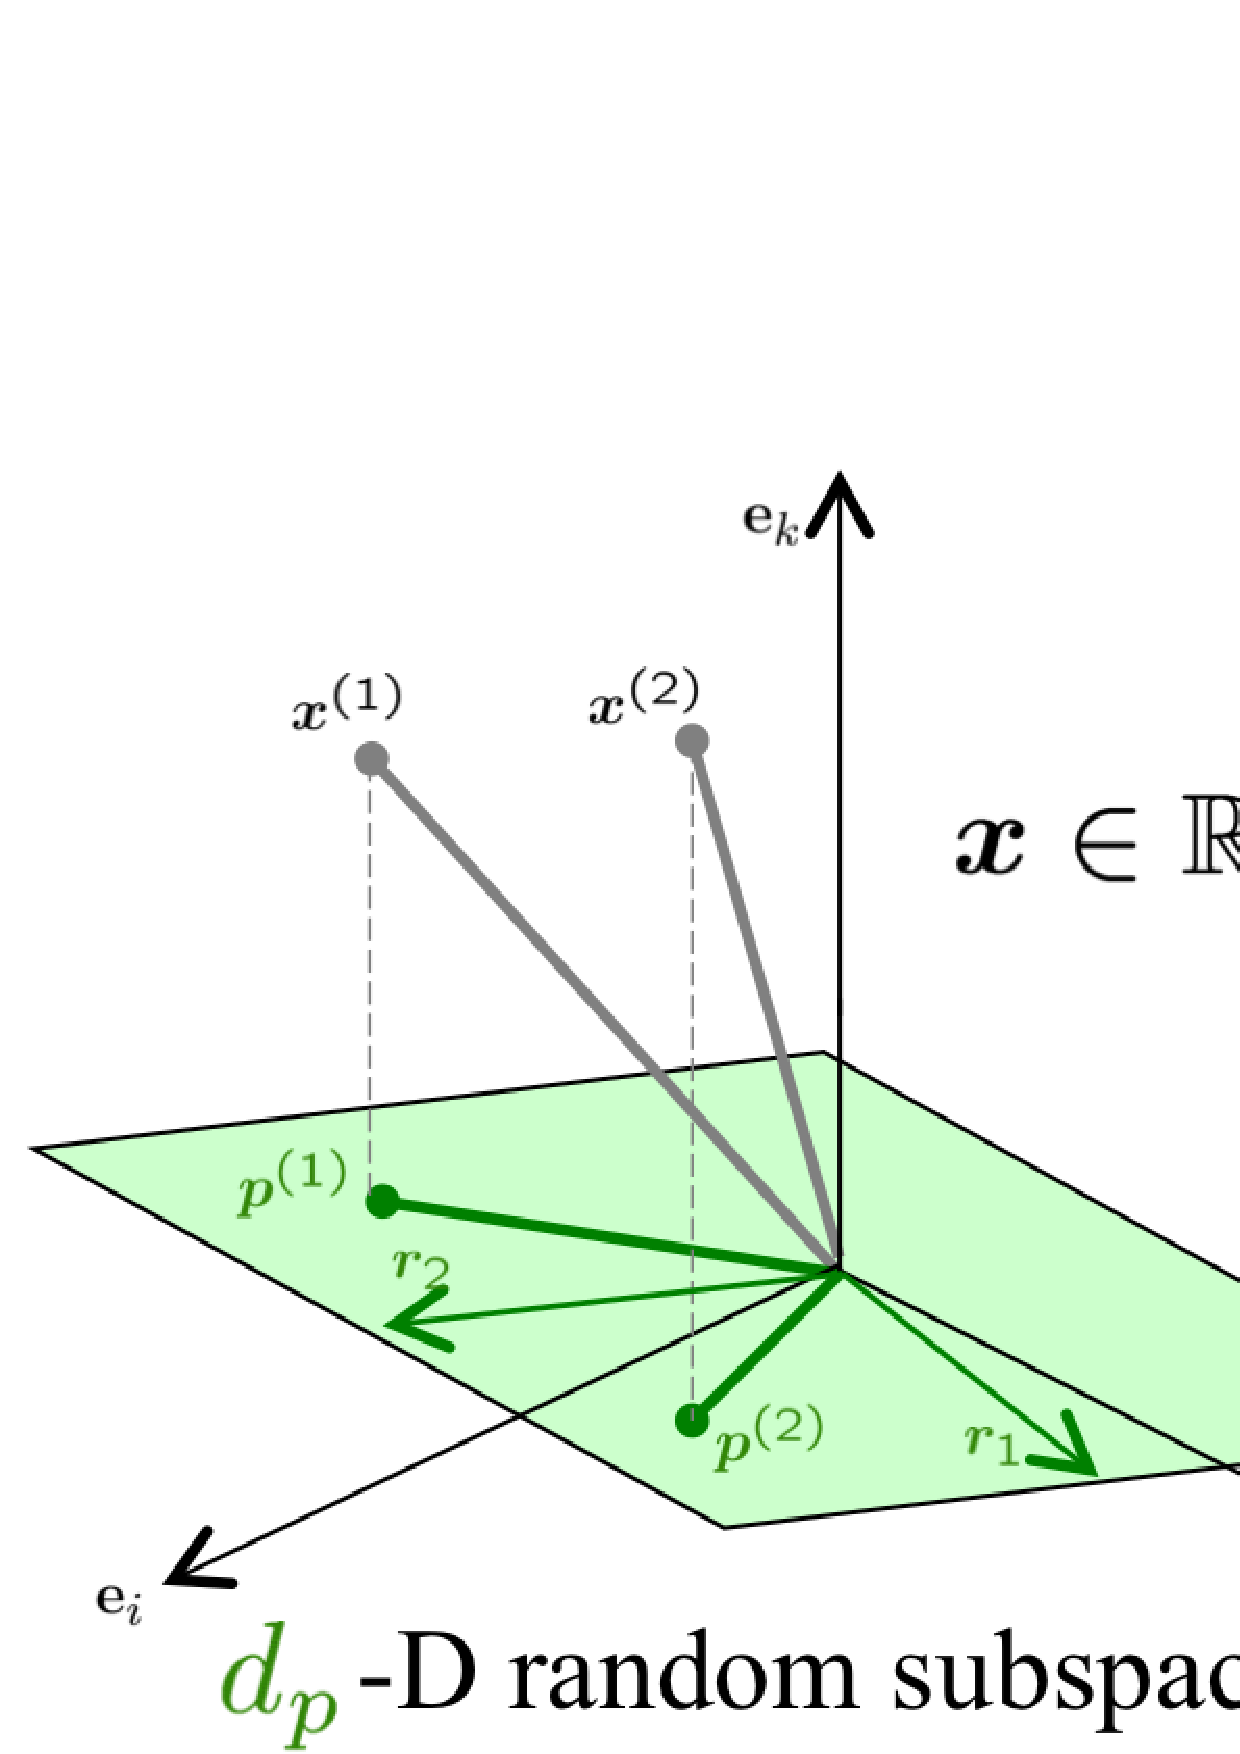
\includegraphics{RP.pdf}}
\put(0,0){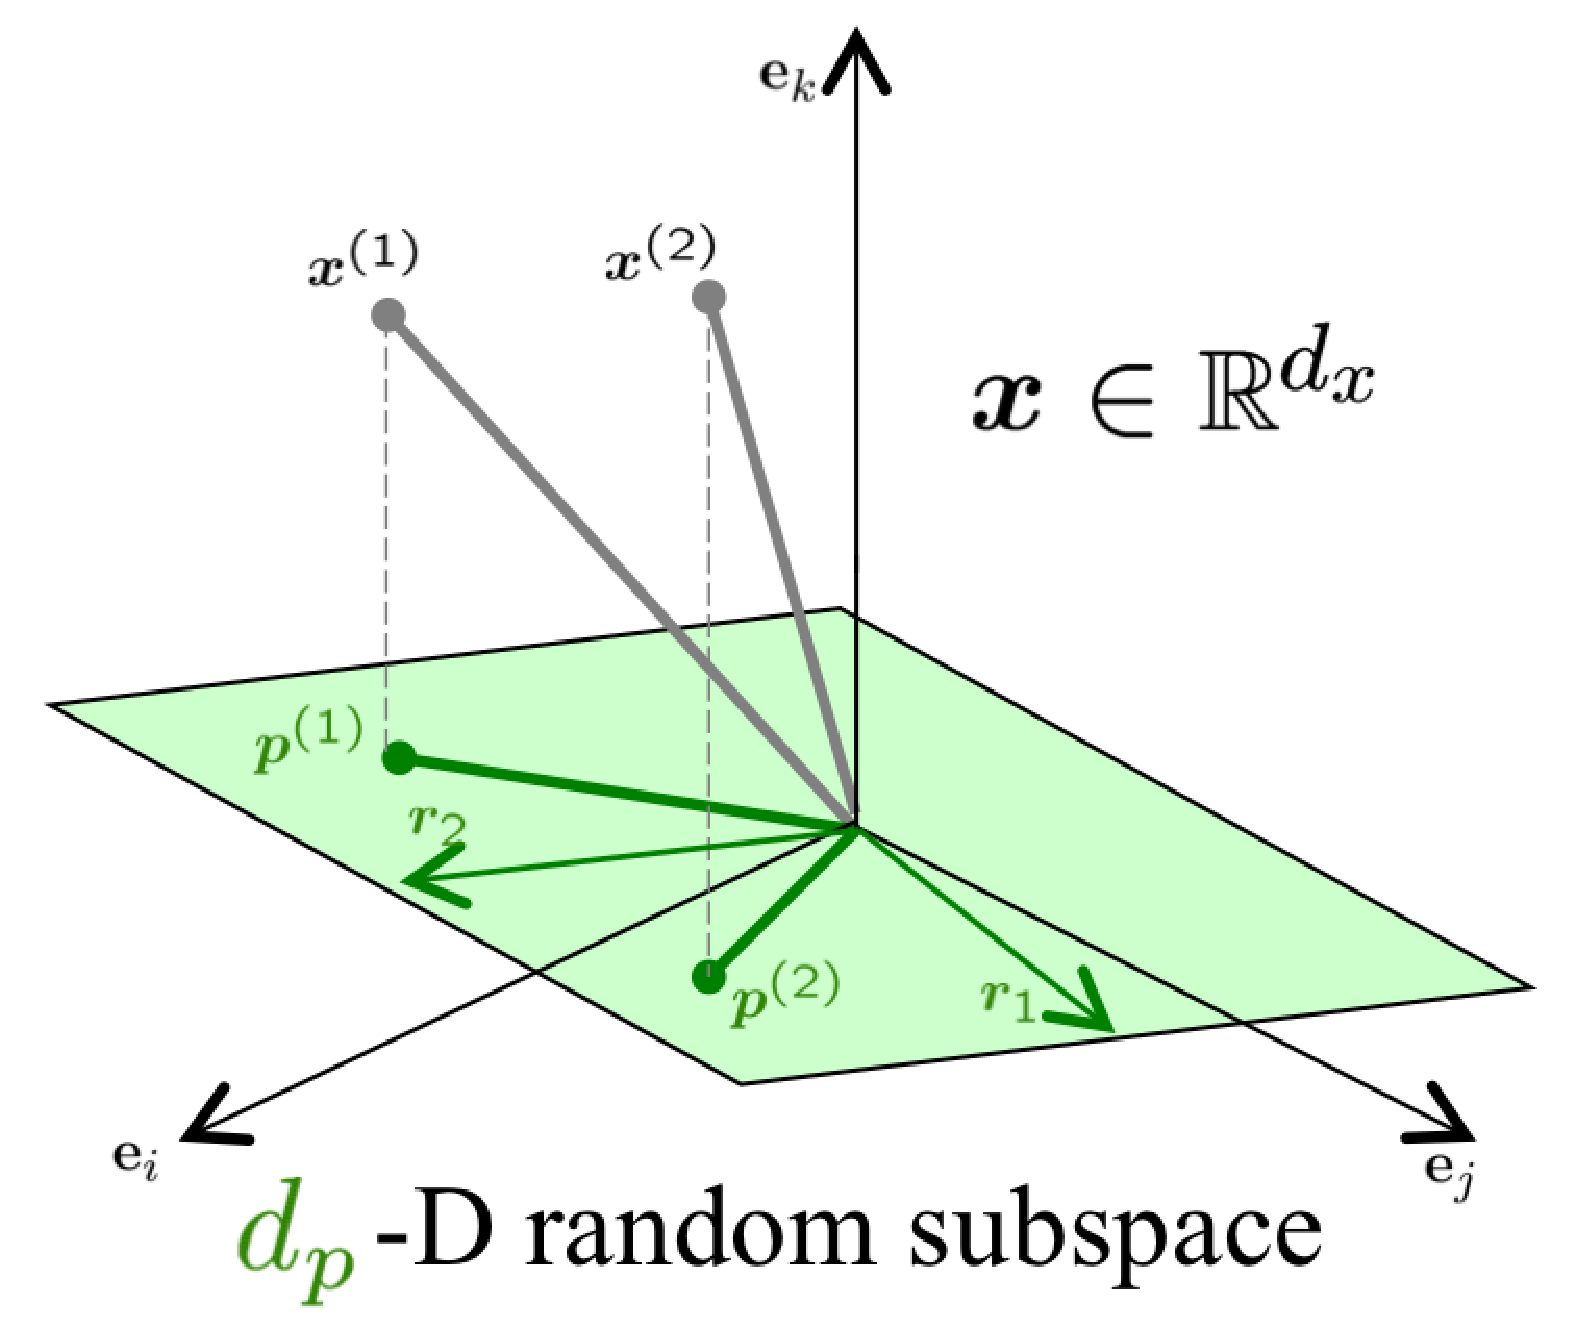
\includegraphics[height=4cm]{RP.eps}}
%\centerline{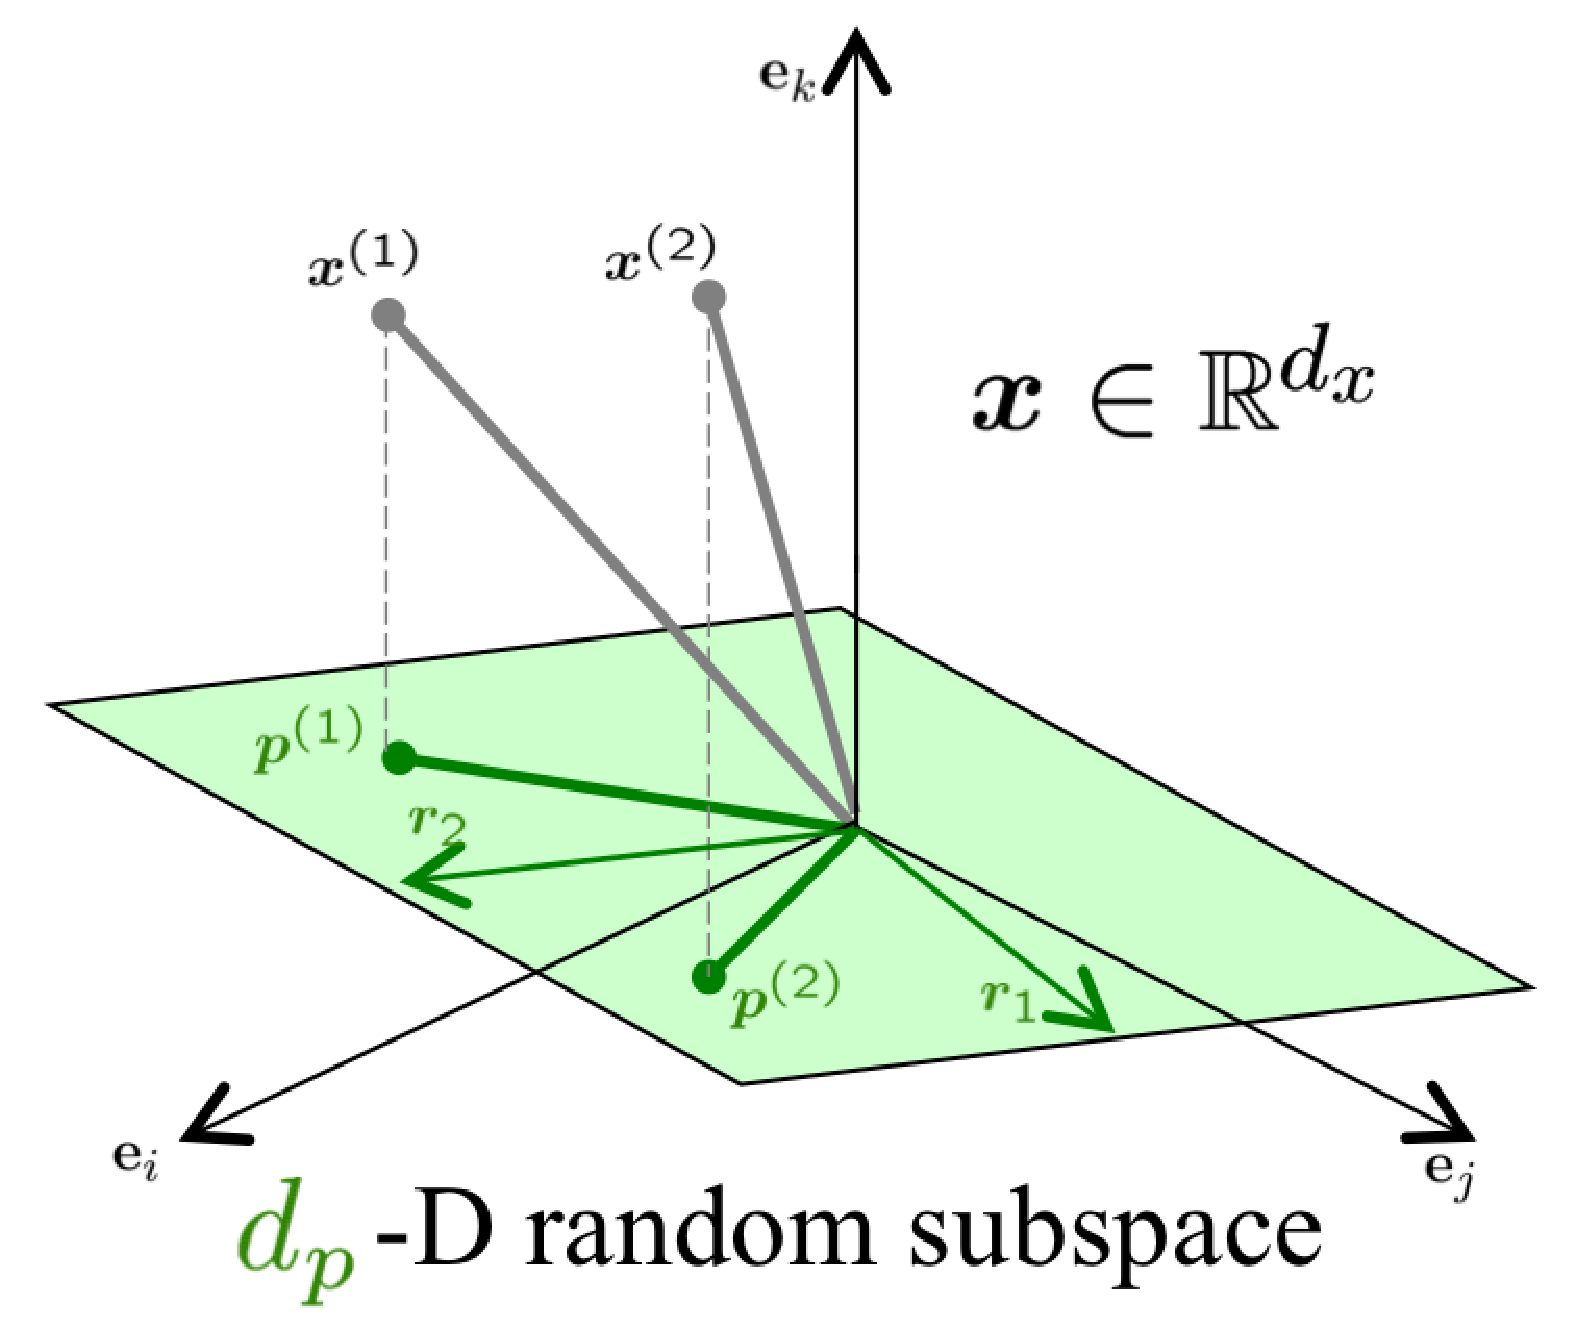
\includegraphics[height=4cm]{RP}}
\end{picture}%}
 \caption{$\vec x\in\mathbb{R}^{d_x}$から$\vec p\in\mathbb{R}^{d_p}$への
ランダム射影.}
\label{fig:RP}
\end{center}
\end{figure}

例えば,平均ゼロ,分散$1/d_p$の正規分布から
ランダム行列$\mtr R$を生成するとしよう.
すると,
$d_x$次元ベクトルで表された
データの集合$X\subset\mathbb{R}^{d_x}$を
ランダム射影した低次元データ集合
$P=\{\vec p\;|\;\vec p=\mtr R\vec x,\vec x\in X\}\subset\mathbb{R}^{d_p}$
は,$X$の様々な性質を高い確率で近似的に保持することが知られている\cite{Vempala04}.
例えば,2本の
ベクトル$\vec x^{(i)},\vec x^{(j)}\in X$をランダム射影した
ベクトルをそれぞれ$\vec p^{(i)},\vec p^{(j)}\in P$とする.
\[
\vec p^{(i)}=\mtr R\vec x^{(i)},\quad \vec p^{(j)}=\mtr R\vec x^{(j)}%,
%\quad\forall \vec x^{(i)},\vec x^{(j)}\in\mathbb{R}^{d_x}.
\]
すると,$\vec p^{(i)}$のノルムは$\vec x^{(i)}$のノルムの良い近似値になる.
同様に,2点$\vec x^{(i)},\vec x^{(j)}\in\mathbb{R}^{d_x}$の間の
距離や内積も高確率で近似的に保存される\footnote{%
$\approx$は近似的に等しいの意味.`≒'の記号を使うのは日本だけらしい(?)}.
\begin{eqnarray}
\|\vec p^{(i)}\|_2 &\approx& \|\vec x^{(i)}\|_2,\\
||\vec p^{(j)}-\vec p^{(i)}||_2 &\approx& ||\vec x^{(j)}-\vec x^{(i)}||_2,\\
{\vec p^{(j)}}^\top\vec p^{(i)} &\approx& {\vec x^{(j)}}^\top\vec x^{(i)}
\end{eqnarray}

ランダム射影で近似的に保存される性質を
図\ref{fig:RP properties}に列挙する.
計量,多様体の構造,2クラス間のマージン,核関数,
主成分等が保存されることが既に解明されている.
\begin{figure}[hb]
\setlength{\unitlength}{1cm}
\begin{center}
%\fbox{
\begin{picture}(14,8)
%\put(0,0){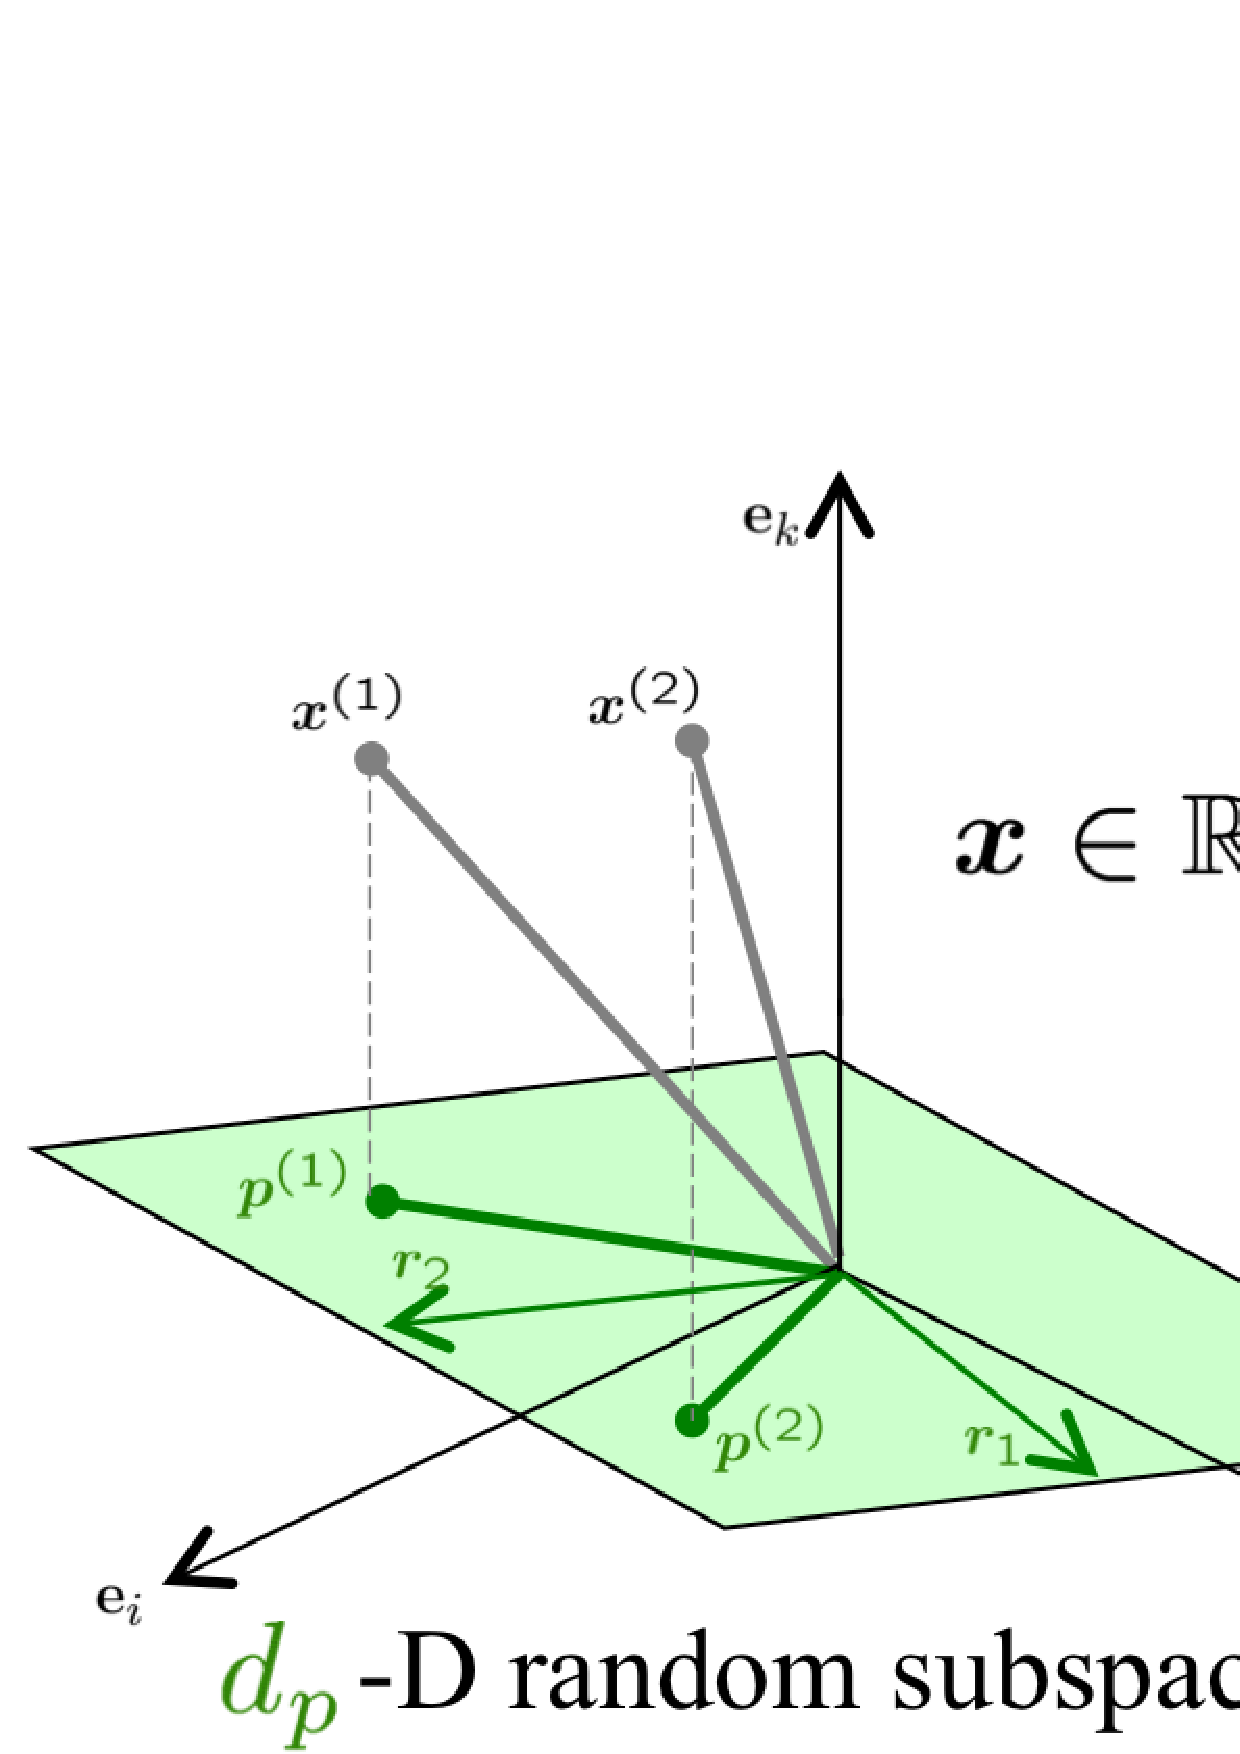
\includegraphics{RP.pdf}}
\put(0,-0.5){\includegraphics[height=8cm]{RPp.eps}}
%\centerline{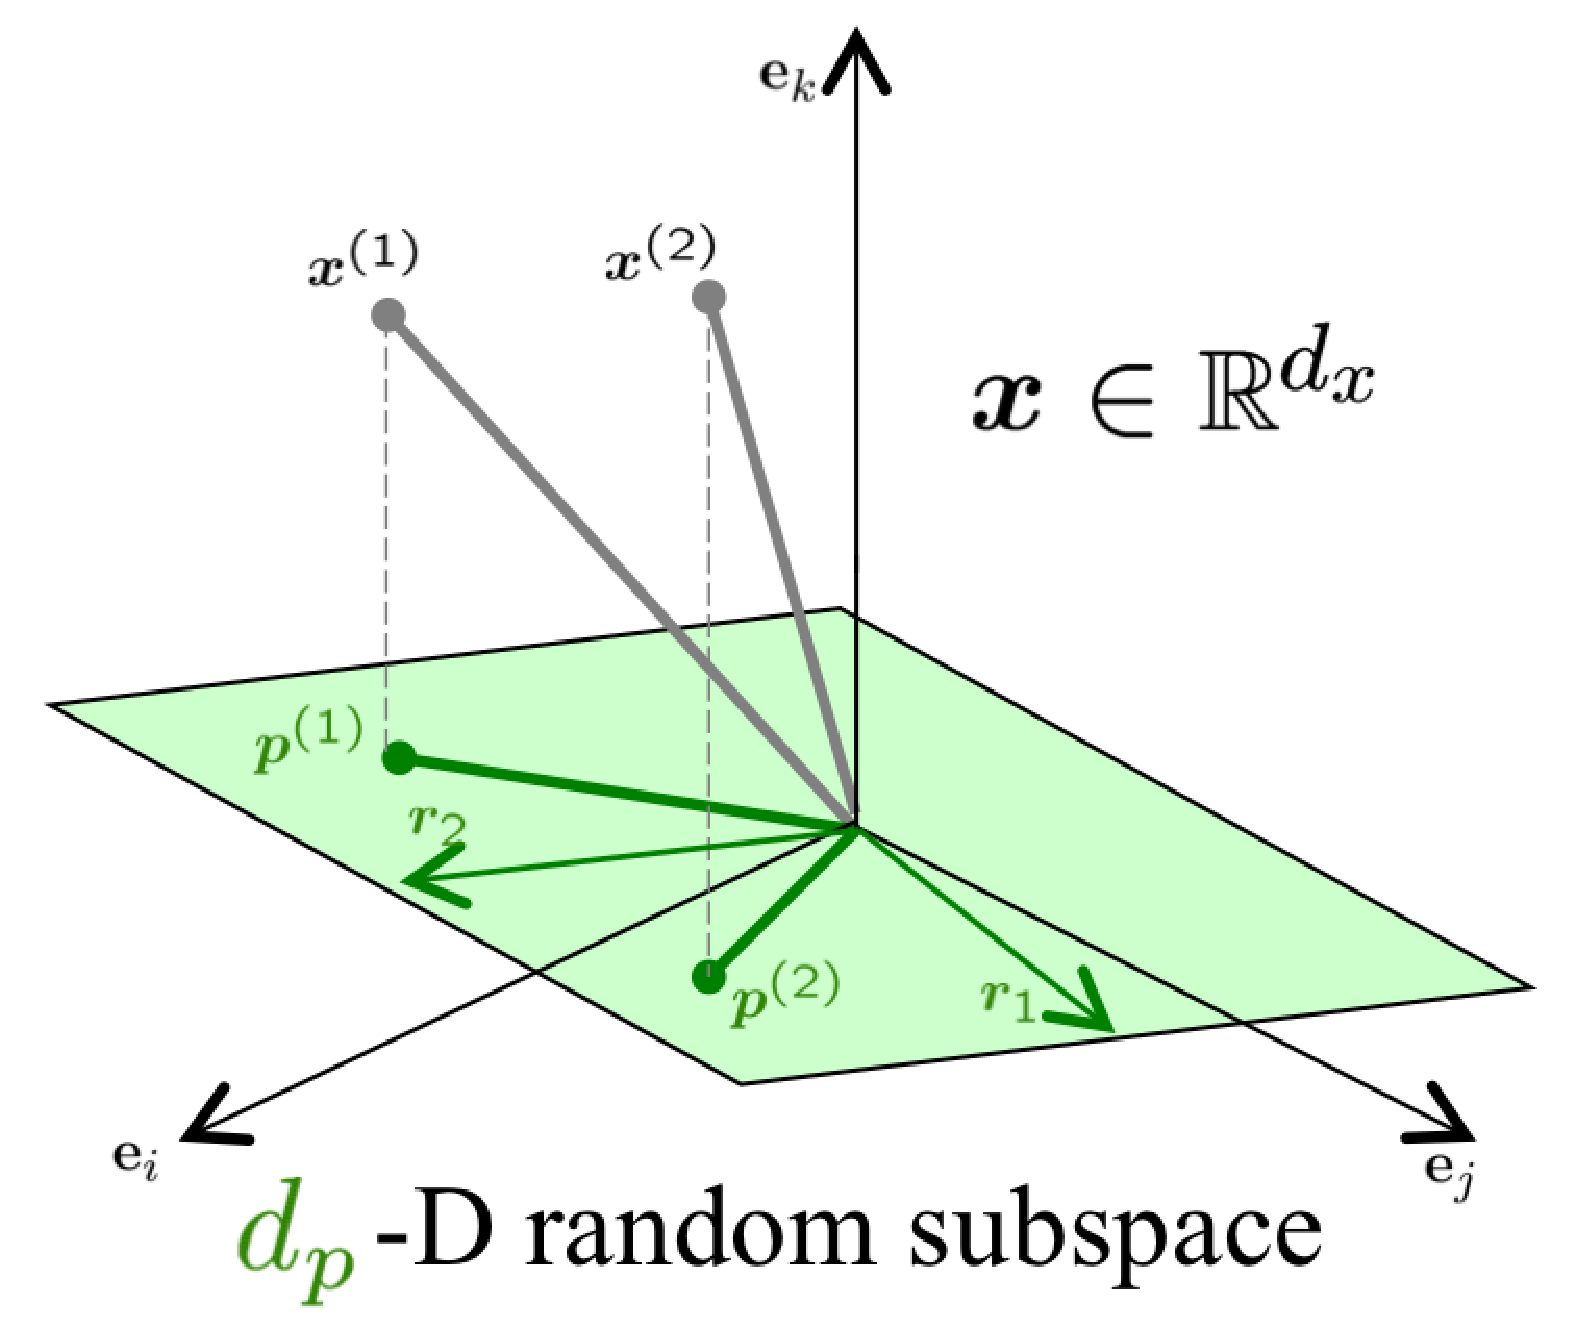
\includegraphics[height=4cm]{RP}}
\end{picture}%}
\end{center}
 \caption{What preserved after random projection.}
\label{fig:RP properties}
\end{figure}


パターン認識(pattern recognition; PR)や機械学習(machine learning; ML)と
呼ばれる研究分野では,
データの特徴を高次元ベクトルで表して分類や予測を達成する
様々な解析手法が設計されている.
内積や距離は,2つのデータの間の類似性・非類似性を測った量と見なせる.
そのような量がランダム射影で近似的に保存されるということは,
低次元データ集合$P$を使って高次元データ集合$X$を解析できることを意味している.
つまり,ランダム射影を使ってPR/MLの計算コストを低減できる
\footnote{ただし,ランダム射影自体の計算コストが問題にならないことが前提である.}.



\Section{試してみよう}

\lstset{language=Matlab}
\lstset{basicstyle={\tt},identifierstyle={\bfseries},keywordstyle={\bfseries}}
\lstset{tabsize=2,showstringspaces=false}
\lstset{commentstyle={\color[rgb]{0,0.5,0}}}
\lstset{flexiblecolumns=true}
\lstset{classoffset=1,breaklines=true,morecomment=[l]{//}}
%\lstset{columns=[l]{fullflexible}}
%\lstset{numbers=left,stepnumber=1,numberstyle={\scriptsize},numbersep=4ex}
\lstset{frame=tBlR,rulecolor={\color[gray]{0.75}},rulesepcolor={\color[gray]{0.75}}}
\lstset{framesep=2ex}
\lstset{xleftmargin=8ex,xrightmargin=16ex}
%\lstset{backgroundcolor={\color[rgb]{1,1,0.95}}}

\paragraph{ノルムを比べてみる}
ランダム射影を実行する単純なMATLABコードを示す.
まず,ランダム行列を作ろう.
\begin{lstlisting}
% データの次元数を設定する.
dx = 10^5;
dp = 300;

% ランダム行列を生成する.
R = randn(dp, dx) / sqrt(dp);
\end{lstlisting}
そして,適当なベクトル{\tt x}を作ってランダム射影を適用する.
\begin{lstlisting}
% ランダムなベクトル x を作成する.
x = randn(dx, 1);

% ランダム射影を計算する.
p = R * x;

% ノルムを表示する.
fprintf('||x|| = %1.3e, ||p|| = %1.3e\n', norm(x), norm(p));
\end{lstlisting}

表示された{\tt x}のノルムとそのランダム射影{\tt p}のノルムが
かなり近い値になっていることが確認できるであろう.
他の次元数(例えば{\tt dp = 1000})でも試してみるとよい.


\paragraph{顔を比べてみる}

顔画像どうしの距離を比べてみよう.
\begin{lstlisting}
% データを読み込む.この例ではYale B cropped face images.
data = load('YaleB_Ext_Cropped_192x168_all.mat');
dx = size(data.fea, 2);
dp = 300;

% ランダム行列を生成する.
R = randn(dp, dx) / sqrt(dp);

% 同一人物の2枚の解画像を表示する.
imshow( reshape(data.fea(100,:), 192, 168) );
imshow( reshape(data.fea(101,:), 192, 168) );

% ランダム射影を計算し,距離を比較する.
x1 = double(data.fea(100,:))';
x2 = double(data.fea(101,:))';
p1 = R * x1;
p2 = R * x2;
fprintf('||x2-x1|| = %1.3e, ||p2-p1|| = %1.3e\n', norm(x2-x1), norm(p2-p1));

% show an image of a different person
imshow( reshape(data.fea(200,:), 192, 168) );

% compute its random projection and compare the distances
x3 = double(data.fea(100,:))';
p3 = R * x3;
fprintf('||x3-x1|| = %1.3e, ||p3-p1|| = %1.3e\n', norm(x3-x1), norm(p3-p1));
\end{lstlisting}


\Section{演習問題}
\begin{enumerate}
\item
適当に作成した$n$本のベクトルについて,
ランダム射影前後のノルムの相対誤差$\varepsilon^{(j)}$を計算せよ.
\[
  \varepsilon^{(j)}=\frac{\|\vec p^{(j)}\|-\|\vec x^{(j)}\|}{\|\vec x^{(j)}\|}\quad (j=1,\dots,n).
\]
\item
相対誤差のヒストグラムを作成し,分布を観察せよ.
ランダム射影先の次元数$d_p$が小さいと誤差はどうなるか.
いくつか異なる次元数$d_p$についてヒストグラムを作成し,観察せよ.\\
ヒント:MATLABでは,{\tt e}をベクトルとすると,
{\tt hist(e,30)}は{\tt e}の成分についてビン数30のヒストグラムを作る.
\item ランダム射影とノルム(または距離)の計算時間を測定せよ.\\
ヒント:{\tt tic; p = R *x; toc}とすると,{\tt p = R * x}の
実行にかかった時間が表示される.
\item\yeeks
計算時間とメモリ使用量がとても少ない
効率的なランダム射影のアルゴリズムがある\cite{Sakai09ERPj,tsakaiAPR11}.
そのアルゴリズムは,サイズ$d_p\times d_x$のランダム行列を生成する必要がない.
どのようなアルゴリズムなのか調べよ.
\item\yeeks
Johnson-Lindenstraussの埋め込み\cite{JL84,Achlioptas03,Dasgupta99,Vempala04}
とは何か調査せよ.
また,ランダム射影後の2点間の距離の誤差に関する命題を見つけ,説明せよ.
\end{enumerate}


%\newpage

{\footnotesize
\bibliography{mybib_rp,mybib_misc}
}

\section*{See also:}
{\footnotesize
\begin{description}
\item[\href{https://drive.google.com/file/d/0Bx4bEpaTSFcgOFA5dVZoZXFkRmc}{[Sakai, 09]}\cite{Sakai09ERPj}]
https://drive.google.com/file/d/0Bx4bEpaTSFcgOFA5dVZoZXFkRmc
\item[\href{https://drive.google.com/file/d/0Bx4bEpaTSFcgZWp2ZDRLa2c1SEE}{[Sakai\&Imiya,11]}\cite{tsakaiAPR11}]
https://drive.google.com/file/d/0Bx4bEpaTSFcgZWp2ZDRLa2c1SEE
\item[\href{http://vision.ucsd.edu/~leekc/ExtYaleDatabase/ExtYaleB.html}{The Extended Yale Face Database B}]
http://vision.ucsd.edu/~leekc/ExtYaleDatabase/ExtYaleB.html\\
cropped images in MATLAB file: \href{https://drive.google.com/file/d/0Bx4bEpaTSFcgRm15NVlua1pOTWM}{YaleB\_Ext\_Cropped\_192x168\_all.mat}\\
https://drive.google.com/file/d/0Bx4bEpaTSFcgRm15NVlua1pOTWM
\end{description}
}


%\bibliographystyle{ieeetr}
%\bibliographystyle{splncs}
%\bibliographystyle{elsart-harv}
%\bibliographystyle{ipsjunsrt-e}
\bibliographystyle{ieicetr}




\Chapter{方程式が足りない!どう解く?--- 劣決定問題と正則化 ---}


\Section{劣決定の線形連立方程式}

未知数の数よりも方程式の数が少ない線形連立方程式(a system of linear equations)を
考えよう.
そのような連立方程式は,無数の解を持ち,解をひとつに決められない問題なので,
%
%\footnote{
%``一般に'' とは ``ほとんどすべて'' を意味する.
%``一般的に正方行列は可逆である.''}
{\bf 劣決定問題}(underdetermined problem)と呼ばれる.

劣決定問題の例を見てみよう.
3個の未知数$x_1,x_2,x_3$\footnote{%
未知数が3個のとき$x,y,z$の記号を使うことに慣れているかもしれないが,
実用上は未知数が$3$個以上あるかもしれないので,本書では添え字付きの記号を使う.}%
に対して2本の方程式しかない連立方程式
\begin{equation}
\smatrix{\small}{rrr}
{1 & 1 & 1\\
1 & 2 & 3}
\smatrix{\small}{c}{x_1\\ x_2\\ x_3}
=
\smatrix{\small}{r}{1\\ 2}
\label{eq:underdetermined example}
\end{equation}
の解は,任意の定数$t\in\mathbb{R}$を使って
\begin{equation}
 \vec x=\smatrix{\small}{c}{x_1\\ x_2\\ x_3}
%=\smatrix{\small}{c}{t\\ 1-2t \\ t}
=\smatrix{\small}{c}{0\\ 1\\ 0}+\smatrix{\small}{c}{1\\ -2\\ 1}t.
\label{eq:solution to the example}
\end{equation}
と表すことができる.
%(式(\ref{eq:underdetermined example})に代入して確認せよ).
$x_1=0,x_2=1,x_3=0$($t=0$)でもよいし,$x_1=1,x_2=-1,x_3=1$($t=1$)でもよい.

連立方程式(\ref{eq:underdetermined example})は,
3次元空間における2つの平面
$x_1+x_2+x_3=1$と$x_1+2x_2+3x_3=2$を表している.
式(\ref{eq:solution to the example})はこの2平面の交わりを表す直線である.
直線は3次元空間の点$[0,1,0]^\top$を通り,方向ベクトルが$[1,-2,1]^\top$である.
この直線上の任意の点$\vec x\in\mathbb{R}^3$すべてが解の候補であり,
与えられた方程式(\ref{eq:underdetermined example})を満たす.
よって,この例は,解が無数に存在し一意に定まらない劣決定問題である.

解を一意に定めるためには,解について更に何か条件が必要である.
例えば,線形方程式がもう1本追加されれば,
3個の未知数に対して方程式が3本になる.
もはや劣決定ではなくなり,3本の線形方程式が表す3平面が交わる1点に
解が定まる.

しかし,式(\ref{eq:underdetermined example})のような劣決定問題に対して,
追加の方程式が全く手に入らないときは,どうしようか.
無数にある解の候補から,ひとつの解を選ぶ合理的な方法はあるだろうか.
方程式の他に,解について何らかの{\bf 事前情報}または{\bf 事前知識}
(prior information/knowledge)を持っているならば,
解を特定する条件としてそれを使えないだろうか.
例えば,「未知数はゼロになるものが多い」という情報を知っていれば,
式(\ref{eq:solution to the example})で表される解の候補の中から
解$\vec x=[0,1,0]^\top$を選べるだろう.
ここでは,解をひとつの絞り込む正則化と呼ばれる手法を紹介しよう.


\Section{線形代数の基礎を少し復習}

\paragraph{連立方程式を行列とベクトルで書き表す}

任意の線形連立方程式は,行列とベクトルを使って
\begin{equation}
 \mtr A\vec x=\vec b
\label{eq:linear system}
\end{equation}
と書き表せる.
ここで,行列$\mtr A\in\mathbb{R}^{m\times n}$と
ベクトル$\vec b\in\mathbb{R}^m$は与えられるものであるとし,
$m$本の連立方程式を表している\footnote{%
例えば,式(\ref{eq:underdetermined example})の連立方程式では,
$\mtr A=\bmatrix{ccc}{1 & 1 & 1\\ 1 & 2 & 3}$,$\vec b=\bmatrix{c}{1\\ 2}$である.}.
ベクトル$\vec x$は$n$個の未知数を成分に持つベクトルである.
連立方程式の本数$m$と未知数の個数$n$によって,
行列$\mtr A$は横長($m<n$),正方($m=n$),縦長($m>n$)のいずれかになる.


\paragraph{連立方程式は線形結合係数を求める問題である}

行列$\mtr A$は,$m$次元ベクトルが列に$n$本並んでいると見ることができる.
本書では,行列$\mtr A$の第$j$列を
$\vec a^{(j)}\in\mathbb{R}^m$と表すことにする.
%$\vec x=[x_1,\dots,x_n]^\top$について
連立方程式(\ref{eq:linear system})は,
与えられた$n$本の$m$次元ベクトル$\vec a^{(j)}$ ($j=1,\dots,n$)を使って,
$m$次元ベクトル$\vec b$を合成するための線形結合係数を求める問題であると解釈できる.
なぜならば,
\begin{equation}
 \vec b=\mtr A\vec x
=\smatrix{\normalsize}{ccc}{\vec a^{(1)} & \dots & \vec a^{(n)}}
\smatrix{\normalsize}{c}{x_1\\ \vdots\\ x_n}
=x_1\vec a^{(1)}+\cdots+x_n\vec a^{(n)}
\label{eq:linear combination}
\end{equation}
と表せるからである.
$n$本の$m$次元ベクトル$\vec a^{(j)}$ ($j=1,\dots,n$)は,
$m$次元ベクトル$\vec b$を線形結合で合成するための{\bf 基底}(basis)
と呼ばれる.

例えば,式(\ref{eq:underdetermined example})の劣決定問題は,
3本の列ベクトル
$\vec a^{(1)}=\smatrix{\small}{c}{1\\ 1},\vec a^{(2)}=\smatrix{\small}{c}{1\\ 2},\vec a^{(3)}=\smatrix{\small}{c}{1\\ 3}$を基底として,
2次元ベクトル$\vec b=\smatrix{\small}{c}{1\\ 2}$を
\[
%\vec b=
\smatrix{\small}{c}{1\\ 2}
%=\smatrix{\small}{ccc}{1 & 1 & 1\\ 1 & 2 & 3}\smatrix{\small}{c}{x_1\\ x_2\\ x_3}
=x_1\smatrix{\small}{c}{1\\ 1}+x_2\smatrix{\small}{c}{1\\ 2}+x_3\smatrix{\small}{c}{1\\ 3}
\]
のように合成するとき,線形結合係数$x_1,x_2,x_3$を求める問題であると解釈できる.
2次元ベクトル$\vec b$を合成するための基底
$\vec a^{(1)},\vec a^{(2)},\vec a^{(3)}$の使い方は,一意に定まらない.
$x_1=0,x_2=1,x_3=0$でもよいし,$x_1=1,x_2=-1,x_3=1$でもよい.
式(\ref{eq:solution to the example})のように,無数に解がある.

\paragraph{ランクとは?}

行列$\mtr A$から線形独立\footnote{%
%$k$本のベクトル$\vec v^{(1)},\vec v^{(2)},\dots,\vec v^{(k)}$の
線形結合
$c_1\vec v^{(1)}+c_2\vec v^{(2)}+\dots+c_k\vec v^{(k)}$について,
$c_1=c_2=\dots=c_k=0$とする以外にゼロベクトルが作れないならば,
$k$本のベクトル$\vec v^{(1)},\vec v^{(2)},\dots,\vec v^{(k)}$は
線形独立であるという.
線形独立な$k$本のベクトルは,ちょうど打ち消しあうことができないので,
どのベクトルもそのベクトルを使わないと作り出せない個性を持っているということ.
}%
な列ベクトルをできるだけ多く選び出したとき,
その列ベクトルの本数を$\mtr A$の{\bf ランク}(rank)と呼び,
$\rank\mtr A$と記す\footnote{階数とも呼ばれる}.
$m$次元ベクトルなので,線形独立なベクトルは高々$m$本である.
$\rank\mtr A=\min(m,n)$のとき\footnote{%
$\min(m,n)$とは,$m$と$n$のどちらか小さい方のことである.
もし$m>n$の場合は$\min(m,n)=n$本までしか列ベクトルを選べないので,
ランクは$\min(m,n)$となる.},
$\mtr A$は{\bf フルランク}(full rank)
であるという.

\paragraph{線形連立方程式が一意の解を持つかどうかは行列$\vec A$の性質次第}

\begin{itemize}
%\begin{description}
\item
%\item[Solution by inverse matrix]
もし,行列$\mtr A$が{\bf 正則}(regular)ならば(逆行列を持つならば),
一意の解$\vec x=\mtr A^{-1}\vec b$が存在する.
\item
%\item[Invertibility]
$\mtr A$が正則である必要十分条件は,
$\mtr A$がフルランクの正方行列であることである.
すなわち,$m=n=\rank\mtr A$である.
正則行列が表す基底は{\bf 完備}(complete)であると呼ばれる.
その理由は,式(\ref{eq:linear combination})のように,
どのようなベクトル$\vec b\in\mathbb{R}^m$も
行列$\mtr A$の$n=m$本の列ベクトルの線形結合で一意に表せるからである.
\item
劣決定の連立方程式,つまり未知数より方程式が少ない場合($m<n$),
解は無数に存在する.
$\mtr A$の$n$本の列ベクトルの線形結合は,
任意の$m$次元ベクトル$\vec b\in\mathbb{R}^m$を表現できるが,
表現が無数に存在する.
行列$\mtr A$は横長であり,次元数$m$よりも基底ベクトルの本数$n$が多い.
$\mtr A$の$n$本の列ベクトルから$m$本をどのように選んでも完備な基底が作れるならば,
そのような横長行列が表す基底は{\bf 過完備}(overcomplete)であると呼ばれる.
\item
{\bf 優決定問題}(overdetermined problem)の連立方程式,
つまり未知数より方程式が多い場合($m>n$)は,一般に「解なし」である\footnote{%
縦長行列$\mtr A$が$\rank\mtr A=n$ならば解なしである.
$\rank\mtr A<n$ならば縦長行列であっても劣決定問題であり,解は無数に存在する.}.
$m$本の方程式から$n$本選んで求めた解$\vec x$は,
選ばなかった他の方程式を満たさないという矛盾が必ず生じる.
$\mtr A$は$m$次元の列ベクトルを$n$本しか持たないので,
任意の$m$次元ベクトル$\vec b$を合成するためには基底が不十分である.

\end{itemize}
%\end{description}


\paragraph{ベクトルのノルムとは?}

ベクトル$\vec x$の大きさを表す非負の実数をノルム(norm)と呼び,
$\|\vec x\|$と表す.
原点Oから位置ベクトル$\vec x$の点までの距離を表すと考えてよい.
しかし,ノルムの測り方は色々ある.
最もよく用いられるノルムは$\ell_2$ノルムである.
$n$次元ベクトル$\vec x=[x_1,x_2,\dots,x_n]^\top\in\mathbb{R}^n$の$\ell_2$ノルムは
$\|\vec x\|_2$と書き表され,下記のように定義されている.
\begin{equation}
\|\vec x\|_2=\sqrt{\vec x^\top\vec x}=\sqrt{x_1^2+\dots+x_n^2}
\label{eq:l2 norm}
\end{equation}
これは,原点と位置ベクトル$\vec x$の点の間のユークリッド距離である.

$\ell_2$ノルム以外にもノルムの定義がある.
例えば,$\vec x$の$\ell_1$ノルムは
\begin{equation}
 \|\vec x\|_1=|x_1|+|x_2|+\dots+|x_n|
\label{eq:l1 norm}
\end{equation}
と定義される.
$\ell_1$ノルムで測った距離はマンハッタン距離(Manhattan distance)
とも呼ばれる.



\Section{正則化の手法}

{\bf 正則化}(regularization)とは,
何らかの条件や情報・事前知識等に基づき,
問題の解をひとつに限定することである.
新たな方程式を追加することなく,
劣決定の連立方程式をどのように正則化できるだろうか.


\paragraph{$\ell_2$最小長さ解}

劣決定の連立方程式は,解$\vec x$のノルムによって単純に正則化できる.
「解$\vec x$は原点Oに近い(ベクトル$\vec x$が短い)ほど良い解である」
という事前知識が正しければ,これを使って最良の解を一意に特定できる.
この解を最小長さ解(minimum length solution)と呼ぶ.

$n$次元空間の原点から点$\vec x\in\mathbb{R}^n$までのユークリッド距離は,
式(\ref{eq:l2 norm})のように$\ell_2$ノルム$\|\vec x\|_2$で測ることができる.
劣決定の連立方程式の解のうち,
原点からのユークリッド距離が最も小さい($\ell_2$ノルムが最も小さい)
最小長さ解を求める問題は,
次のような最小化問題として記述できる.
\begin{equation}
 \min_{\small\vec x}\|\vec x\|_2^2\quad\mbox{ subject to }\quad
\mtr A\vec x=\vec b.
%\|\vec b-\mtr A\vec x\|\leq\delta.
\label{eq:minimum length solution}
\end{equation}
%where $\delta\geq 0$ is a tolerance.
この記述は,
「$\vec x$の$\ell_2$ノルムの2乗$\|\vec x\|_2^2$の最小値を求めよ.
ただし,$\vec x$は$\mtr A\vec x=\vec b$を満たすものとする.」
という意味である.
式(\ref{eq:minimum length solution})の最小値から決まる
一意の解$\vec x^*$は,
$\mtr A$と$\vec b$を使って書き表すことができる
(演習問題\ref{ex:min l2 solution}).
\begin{equation}
\vec x^*=\mtr A^\top(\mtr A\mtr A^\top)^{-1}\vec b
\label{eq:MLS}
\end{equation}


\paragraph{$\ell_2$正則化}

$\ell_2$最小長さ解と似ているが,
少し異なる別の正則化の手法として,$\ell_2$正則化を紹介しよう.
$\ell_2$正則化は,連立方程式から解$\vec x$がずれている量(誤差)と,
解の$\ell_2$ノルムの2乗$\|\vec x\|_2^2$を,一緒に最小化する.
\begin{equation}
 \min_{\small\vec x} \frac{1}{2}\|\vec b-\mtr A\vec x\|_2^2
+\lambda \|\vec x\|_2^2
\label{eq:l2 regularization}
\end{equation}
この記述は,
「$\vec b$と$\mtr A\vec x$のずれの大きさ$\|\vec b-\mtr A\vec x\|_2^2$と,
$\vec x$の長さを表す量$\lambda\|\vec x\|_2^2$を計算した.
$\vec x$を調節して,この和の最小値を求めよ.」という意味である.
$\ell_2$正則化は,統計学の分野で{\bf リッジ回帰}(ridge regression)として知られている.
式(\ref{eq:l2 regularization})から決まる一意の解$\vec x^*$も,
$\mtr A$,$\vec b$,$\lambda$を使って書き表すことができる
(演習問題\ref{ex:l2 regularization})%
\footnote{式(\ref{eq:l2 regularization})に$\frac{1}{2}$が付いていなければ
$\vec x^*=(\mtr A^\top\mtr A+\lambda\mtr I)^{-1}\mtr A^\top\vec b$
が最小解である.}.
\begin{equation}
\vec x^*=(\mtr A^\top\mtr A+2\lambda\mtr I)^{-1}\mtr A^\top\vec b
\label{eq:l2 ridge}
\end{equation}


式(\ref{eq:l2 regularization})の最小値から決まる解$\vec x$は,
もはや$\mtr A\vec x=\vec b$を厳密には満たさない.
$\vec b$と$\mtr A\vec x$のずれの大きさ$\|\vec b-\mtr A\vec x\|_2^2$
は{\bf 損失関数}(loss function)と呼ばれる.
$\ell_2$ノルムで測った誤差と考えてよい.
%$\hat{\vec b}=\mtr A\vec x$で$\vec b$を近似したときの
%誤差と考えてよい.
正の定数$\lambda\in\mathbb{R}_+$は,
損失関数と解の$\ell_2$ノルムのどちらも小さくなるようにバランスをとる役割があり,
あらかじめ適切な値を設定しておく必要がある.
設定した$\lambda$が小さいほど,
損失関数が小さい(連立方程式を近似的に良く満たす)解が選ばれるようになるが,
$\ell_2$ノルムが小さい解が選ばれ難くなる(つまり事前知識が活かされない).
逆に,設定した$\lambda$が大きいほど,
解の$\ell_2$ノルムが小さいという事前知識が重視されるが,
損失関数があまり小さくない(連立方程式をあまり満たさない)解が選ばれるようになる.


無数の解の候補のうち,$\ell_2$ノルムが小さいものを選ぶことは適切なのだろうか.
連立方程式に帰着する何かの応用問題で,もし$\vec x$の成分が
物理量(例えば電流や電圧,速度等)を表しているならば,
式(\ref{eq:l2 norm})のような2乗和はエネルギーに相当するので,
$\ell_2$最小長さ解はエネルギーが最小の解を選んでいると解釈できるかもしれない.
しかし,式(\ref{eq:l1 norm})の$\ell_1$ノルムのように,
$\ell_2$以外のノルムを用いた正則化も非常に重要であり,
科学技術の様々な分野で次々と革新的な成果を生んでいる.
次回はそのような正則化を紹介しよう.




\Section{演習問題}
\begin{enumerate}

\item
式(\ref{eq:underdetermined example})の劣決定問題の$\ell_2$最小長さ解を求めよ.\\
ヒント:解は$t$を使って式(\ref{eq:solution to the example})のように表される.
$\|\vec x\|_2^2$は$t$の2次関数になる.これが最小となる$t$を求めよ.

\item\yeeks\label{ex:min l2 solution}
劣決定問題
$\mtr A\vec x=\vec b$
($\mtr A\in\mathbb{R}^{m\times n}$, $m<n$)について,
$\ell_2$最小長さ解
\begin{equation}
 \vec x^*=\arg\min_{\small\vec x}\|\vec x\|_2^2\quad\mbox{ subject to }\quad \mtr A\vec x=\vec b
\end{equation}
は,$\mtr A$と$\vec b$を用いて
式(\ref{eq:MLS})のように陽に書き表せることを示せ.\\
ヒント:ラグランジュ乗数法(the Lagrange multiplier method)を適用する.
最小長さ解は,下記のラグランジュ関数の停留点である.
\[
 L(\vec x,\vec\lambda)=\frac{1}{2}\vec x^\top\vec x+\vec\lambda^\top(\vec b-\mtr A\vec x).
\]

\item
式(\ref{eq:underdetermined example})の劣決定問題について,
$\vec x^*=\mtr A^\top(\mtr A\mtr A^\top)^{-1}\vec b$を計算せよ.
$\vec x^*$は$\ell_2$最小長さ解である.


\item\yeeks\label{ex:l2 regularization}
劣決定問題
$\mtr A\vec x=\vec b$
($\mtr A\in\mathbb{R}^{m\times n}$, $m<n$)について,
$\ell_2$正則化問題の解
\begin{equation}
 \vec x^*=\arg\min_{\small\vec x} \frac{1}{2}\|\vec b-\mtr A\vec x\|_2^2+\lambda \|\vec x\|_2^2
\end{equation}
は,$\mtr A$,$\vec b$,$\lambda$を用いて
式(\ref{eq:l2 ridge})のように陽に書き表せることを示せ.\\
ヒント:$\vec x$のすべての成分について偏微分してゼロと置く.
{\bf 勾配}(gradient),
{\bf リッジ回帰}または{\bf チホノフ正則化}(Tikhonov regularization)について調査せよ.

\item\yeeks\label{ex:least squares}
優決定問題
$\mtr A\vec x=\vec b$
($\mtr A\in\mathbb{R}^{m\times n}$, $m>n$)の解は一般に存在しない.
$\ell_2$ノルムで測った誤差$\|\vec b-\mtr A\vec x\|_2$を最小にする$\vec x$を
近似解とする手法は{\bf 最小二乗法}(least squares method)と呼ばれる.
最小二乗解
\begin{equation}
 \vec x^*=\arg\min_x\|\vec b-\mtr A\vec x\|_2^2
\end{equation}
は,$\mtr A$と$\vec b$を用いて
\begin{equation}
 \vec x^*=(\mtr A^\top\mtr A)^{-1}\mtr A^\top\vec b
\end{equation}
のように陽に書き表せることを示せ.



\end{enumerate}


%\bibliographystyle{ieeetr}
%\bibliographystyle{splncs}
%\bibliographystyle{elsart-harv}
%\bibliographystyle{ipsjunsrt-e}
\bibliographystyle{ieicetr}




\Chapter{多すぎるのは良くないことだ --- 劣決定問題のスパース解 ---}

{\bf 劣決定問題}(underdetermined problem)が解ければ,
例えばこんなことができるぞ.
%\begin{figure}[hb]
\setlength{\unitlength}{1cm}
\begin{center}
%\fbox{
\begin{picture}(17,18.2)
\put(0,-3){\includegraphics[width=17cm]{cs_applications.eps}}
\end{picture}%}
\end{center}
% \caption{What preserved after random projection.}
%\label{fig:CS applications}
%\end{figure}

\clearpage


\Section{劣決定問題のスパース正則化}

\paragraph{前回までのあらすじ}

\begin{enumerate}
\item
線形連立方程式は,行列とベクトルを使って
\begin{equation}
\mtr A\vec x=\vec b
\label{eq:linear system A}
\end{equation}
と書き表せる.
$\vec x\in\mathbb{R}^n$は$n$個の未知数を成分に持つ$n$次元ベクトルである.
$\mtr A\in\mathbb{R}^{m\times n}$は,
$m$本の方程式における未知数の係数を要素に持つ$m\times n$行列である.
$\vec b\in\mathbb{R}^m$は,$m$個の定数を成分に持つ$m$次元ベクトルである.

\item
連立方程式(\ref{eq:linear system A})は,
行列$\mtr A$の$n$本の列ベクトル$\vec a^{(j)}$ ($j=1,\dots,n$)を
基底に使って$\vec b$を合成するための線形結合係数を求める問題であると解釈できる.
なぜならば,
\begin{equation}
 \vec b=\mtr A\vec x
=\smatrix{\normalsize}{ccc}{\vec a^{(1)} & \dots & \vec a^{(n)}}
\smatrix{\normalsize}{c}{x_1\\ \vdots\\ x_n}
=x_1\vec a^{(1)}+\cdots+x_n\vec a^{(n)}
\label{eq:linear combination A}
\end{equation}
と表せるからである.

\item
未知数の数よりも方程式の数が少ない連立方程式は,無数の解を持ち,
解をひとつに決められない劣決定問題である.
%それ以上の方程式が手に入らないとき,
%無数にある解の候補から,ひとつの解を合理的に選ぶ方法はあるだろうか.
方程式の他に,解に関する情報や事前知識があるとき,
それを使って解をひとつに限定することを正則化と呼ぶ.
\end{enumerate}

方程式が足りなくても,正則化で正解が得られるならば,
$n$個の未知数について$m=n$本の方程式を用意するのは無駄ではなかろうか.
どのような方程式の解について事前知識がある場合に,
方程式が足りなくても正解が得られることを保証できるだろうか.




\paragraph{スパース解}

「未知数はゼロになるものが多い」という事前知識は,非常に重要な正則化になる.
無数に存在する解のうち,非ゼロとなる未知数の数が最も少ない
(ゼロになる未知数がの数が最も多い)解を求める問題は,
次のような最小化問題として定式化される.
\begin{equation}
 \min_{\small\vec x}\|\vec x\|_0\quad\mbox{ subject to }\quad \mtr A\vec x=\vec b
\label{eq:sparse solution}
\end{equation}
%\begin{equation}
% \min\; \#\{i|x_i\neq 0\}\quad\mbox{ subject to }\quad \mtr A\vec x=\vec b
%\label{eq:sparse solution}
%\end{equation}
この記述は,
「ベクトル$\vec x$の成分のうち,ゼロでないものの個数$\|\vec x\|_0$の最小値を求めよ.
ただし,$\vec x$は$\mtr A\vec x=\vec b$を満たすものとする.」
という意味である.
$\|\vec x\|_0$は,$\vec x$の$\ell_0$ノルムと呼ばれ,
$\vec x$の非ゼロ成分の個数を表す
\footnote{%
これは便宜上の記述である(演習問題\ref{ex:l0 norm}).
正確には下記のように記述すべきである.
\[
 \min_{\scriptsize\vec x}\lim_{p\rightarrow 0}\|\vec x\|_p^p\quad\mbox{subject to}\quad \mtr A\vec x=\vec b
\]
}.
すなわち,$\|\vec x\|_0=|\{i|x_i\neq 0\}|$
(ゼロでない成分の集合の要素の数)と定義する.

式(\ref{eq:sparse solution})の解を{\bf スパース解}(sparse solution)と呼ぶ.
また,ベクトルの非ゼロ成分の数が$k$個以下の場合,
そのベクトルは$k$スパース($k$-sparse)であると言う.
式(\ref{eq:linear combination A})のように,
$\vec x$は線形結合係数を成分に持つベクトルであるから,
スパース解の非ゼロ成分に対応する$\mtr A$の列ベクトルのみによって
ベクトル$\vec b$が簡潔に表現される.
%これを,$\vec b$のスパース表現と呼ぶ.
%スパース解は,$\mtr A$の列ベクトルのうち,
%なるべく少ない本数で$\vec b$を合成する問題の解である.
よって,式(\ref{eq:sparse solution})の$\ell_0$最小化問題は,
$\mtr A$の列から最少の本数で$\vec b$を合成できる
組合せを探すというNP困難な「組合せ最適化問題」である.
また,式(\ref{eq:sparse solution})の解は必ずしも一意ではない.


数学では,
関数$f(x)$の値がゼロにならないような$x$の集合を,
その関数の{\bf 台}(support)と呼ぶ.
同様に,ベクトルの非ゼロ成分の番号(添え字)の集合を,ベクトルの台と呼ぶ.
$1$から$n$までの整数の集合を$[n]=\{1,\dots,n\}$と表すならば,
$n$次元ベクトルの台$S$は集合$[n]$の部分集合である($S\subset[n]$).
また,非ゼロ成分の個数はこの集合の要素の数$|S|$である.
\begin{description}
\item[例]
$\vec x=[0,2,0,0,1]^\top$の台は$S=\{2, 5\}$である($x_2\neq 0,x_5\neq 0$).
もちろん,$S\subset[5]=\{1,2,3,4,5\}$が成り立つ.
\end{description}

本書では,$n$本の列を持つ行列$\mtr A\in\mathbb{R}^{m\times n}$について,
番号の集合を$T\subset[n]$とするとき,
$T$で指定した$\mtr A$の列を抜き出して作った$m\times |T|$行列を
$\mtr A_T$と記すことにする.
同様に,
$T$で指定した番号の成分を$\vec x$から抜き出して作った$|T|$次元ベクトルを
$\vec x_T$と記す.
\begin{description}
\item[例]
$\mtr A=\smatrix{\small}{ccc}{1 & 1 & 1\\ 1 & 2 & 3}$,$\vec x=[0,1,2]^\top$,
$T=\{1, 3\}$のとき,
$\mtr A_T=\smatrix{\small}{cc}{1 & 1\\ 1 & 3}$,
$\vec x_T=\smatrix{\small}{c}{0\\ 2}$である.
\end{description}



\Section{スパース解が一意になる条件}

スパース解を求める方法を考える前に,
式(\ref{eq:sparse solution})のスパース解が
複数存在せず一意に定まる条件は何なのか知っておきたい.
式(\ref{eq:sparse solution})の$k$スパース解の一意性は,
$\mtr A$の列ベクトルの組合せの線形独立性に依存している.


\paragraph{単純な例で考察しよう}

次のような$4\times 5$の行列で考えてみよう.
\begin{equation}
\mtr A\msup{n}=\smatrix{\small}{ccccc}
{
1 & 0 & 1 & 0 & 0\\
0 & 1 & 1 & 0 & 0\\
0 & 1 & 1 & 1 & 0\\
0 & 0 & 1 & 0 & 1}\quad\mbox{and}\quad
\mtr A\msup{u}=\smatrix{\small}{ccccc}
{
1 & 0 & 1 & 0 & 0\\
0 & 1 & 2 & 0 & 0\\
0 & 1 & 1 & 1 & 0\\
0 & 0 & 1 & 0 & 1}.
\label{eq:Spark4Spark5}
\end{equation}
これらはフルランクである($\rank\mtr A\msup{n}=4$,$\rank\mtr A\msup{u}=4$).
行列の列の組合せを見てみよう.4本の列を選ぶとする.
行列$\mtr A\msup{n}$には,線形独立にならない4本の列の組合せが存在する.
第1,2,3,5列という組合せである(第1,2,5列を足し合わせると第3列が作れてしまう).
一方,$\mtr A\msup{u}$は,どの4本の列を組合せても必ず線形独立になる.

まず,$\mtr A=\mtr A\msup{n}$,$\vec b=[1,1,1,0]^\top$として,
式(\ref{eq:sparse solution})のスパース解を見つけてみよう.
解$\vec x$は,式(\ref{eq:linear combination A})のように
$\vec b$を合成するための線形結合係数なので,
スパース解の台は合成に使用する$\mtr A\msup{n}$の列に対応する.
$\mtr A\msup{n}$の$n=5$本の列から線形独立な$m=4$本のベクトルを選べば,
どんな4次元ベクトルも合成できる.
${}_5$C${}_4=5$通りの列の組合せのうち,
線形独立な列ベクトルの組合せは$4$通りある.
$T=\{1,2,3,4\}$,$\{1,2,4,5\}$,$\{1,3,4,5\}$,$\{2,3,4,5\}$である.
これら$4$通りの組合せから$4$通りの解が得られる\footnote{%
例えば,$T=\{2,3,4,5\}$ならば,
$\mtr A\msup{n}$の第1列を使用しないから$x_1=0$である.
$\mtr A_T\msup{n}\vec x_T=\vec b$の方程式から
$\vec x_T=[x_2,x_3,x_4,x_5]^\top=[0,1,0,-1]^\top$を得る.}.
%\footnote{%
%$\mtr A_T\vec x_T=\vec b$という4通りの方程式が作れる.
%それぞれの方程式から,$T$で指定された$\vec x$の成分が求まる.
%$T$以外の列は使っていないので,それ以外の$\vec x$の成分は0である.
%}.
\begin{equation}
 \vec x=
\smatrix{\small}{r}{1 \\ 1 \\ 0 \\ 0 \\ 0},\quad
\smatrix{\small}{r}{1 \\ 1 \\ 0 \\ 0 \\ 0},\quad
\smatrix{\small}{r}{0 \\ 0 \\ 1 \\ 0 \\ -1},\quad
\smatrix{\small}{r}{0 \\ 0 \\ 1 \\ 0 \\ -1}
\end{equation}
この結果から,解はスパースであるが,2種類存在することがわかる.
ゆえに,$\mtr A\msup{n}$は$\vec b$に対して一意のスパース解を持たない.
$\vec b$を簡潔に合成するためには,
$\mtr A\msup{n}$の第1列と第2列の組合せでもよいし,
第3列と第5列の組合せでもよいということを2種類のスパース解が示している.
つまり,$\mtr A\msup{n}$の過完備基底のように,
互いに代用可能な基底ベクトルの組合せが存在するとき,解が一意にならない.



次に,$\mtr A=\mtr A\msup{u}$,$\vec b=[1,1,1,0]^\top$として,
同様にスパース解を見つけててみよう.
$4$本選ぶ列の組合せは${}_5$C${}_4=5$通りあるが,どれも線形独立になる.
$T=\{1,2,3,4\}$,$\{1,2,3,5\}$,$\{1,2,4,5\}$,$\{1,3,4,5\}$,$\{2,3,4,5\}$
の$5$通りの組合せから,それぞれ次のような解が得られる.
\begin{equation}
\vec x=
\smatrix{\small}{r}{1 \\ 1 \\ 0 \\ 0 \\ 0},\quad
\smatrix{\small}{r}{1 \\ 1 \\ 0 \\ 0 \\ 0},\quad
\smatrix{\small}{r}{1 \\ 1 \\ 0 \\ 0 \\ 0},\quad
\smatrix{\small}{r}{0.5 \\ 0 \\ 0.5 \\ 0.5 \\ -0.5},\quad\mbox{and}\quad
\smatrix{\small}{r}{0 \\ -1 \\ 1 \\ 1 \\ -1}
\label{eq:solutions to A5}
\end{equation}
ゆえに,$\mtr A\msup{u}$は$\vec b$に対して
一意の$k=2$スパース解$\vec x=[1,1,0,0,0]^\top$を持つ.
$\mtr A\msup{u}$の第1列と第2列の組合せだけが$\vec b$を簡潔に合成できる.
$\mtr A\msup{u}$の過完備基底は,
互いに代用可能な基底ベクトルの組合せが存在しないので,解が一意になる.



\Subsection{スパース解が一意になるための十分条件}

\paragraph{スパーク}
\begin{definition}
行列$\mtr A$から,
線形独立に{\bf ならない}列ベクトルをなるべく少なく選び出したとき,
その列ベクトルの本数を$\mtr A$の{\bf スパーク}(spark)と呼び,
$\spark\mtr A$と記す.
\begin{equation}
 \spark\mtr A=\min_{\small\vec x\neq\vec 0}\|\vec x\|_0
\quad\mbox{subject to}\quad\mtr A\vec x=\vec 0.
\end{equation}
\end{definition}
\begin{theorem}
\label{th:uniqueness}
$\spark\mtr A>2k$ならば,式(\ref{eq:sparse solution})の$k$スパース解は一意である.
\end{theorem}
\noindent
この証明は演習問題\ref{ex:uniqueness}とする.

スパークはランクに似ているが混同しないように注意されたい.
例えば,式(\ref{eq:Spark4Spark5})の行列$\mtr A\msup{n}$と$\mtr A\msup{u}$は,
ランクがどちらも$\rank\mtr A\msup{n}=\rank\mtr A\msup{u}=4$であるが,
スパークは$\spark\mtr A\msup{n}=4$,$\spark\mtr A\msup{u}=5$である.
ただし,スパークを求める問題は,線形独立にならない列の組合せを探す
組合せ問題である
(演習問題\ref{ex:spark is comb}).
定理\ref{th:uniqueness}から,
$\mtr A\msup{u}$の$k=2$スパース解は一意であると言える.



\paragraph{制限等長性}
\begin{definition}
任意の$k$スパースなベクトル$\vec x$について不等式
\begin{equation}
(1-\delta)\|\vec x\|_2^2\leq\|\mtr A\vec x\|_2^2\leq(1+\delta)\|\vec x\|_2^2.
\label{eq:RIP}
\end{equation}
を満たす定数$\delta<1$が存在するとき,
行列$\mtr A\in\mathbb{R}^{m\times n}$は$k$次の
{\bf 制限等長性}(restricted isometry property; RIP)を持つという.
この性質を$(\delta,k)$-RIPと表す.
等価な定義として,
$k$個以下の要素を持つ任意の部分集合$S\subset[n]$ ($|S|\leq k$)について不等式
\begin{equation}
 \|\mtr A_S^\top\mtr A_S-\mtr I_k\|_2\leq\delta
\end{equation}
が成り立つとき,行列$\mtr A$は$(\delta,k)$-RIPの制限等長性を持つという.
ここで,$\mtr I_k$は$k\times k$の単位行列である.
\end{definition}
言い換えると,$(\delta,k)$-RIP条件を満たす行列$\mtr A$による線形写像は,
$k$スパースな任意のベクトルのノルムを近似的に維持する.
この性質は,ランダム射影のそれと同様である.
実際,$k$スパースなベクトルの幾何(ノルムや距離)を
維持するようにJLの補題\cite{JL84}を適用すると,
$m\times n$のランダム行列$\mtr A$について
\begin{equation}
 m> m_0\approx\frac{1}{\delta^2}k\log\frac{n}{k}
\label{eq:random projection with RIP}
\end{equation}
が成立するならば,
$\mtr A$は$(\delta,k)$-RIP条件を満たす(演習問題\ref{ex:JL RIP}).
また,もし$\mtr A$が$(\delta,2k)$-RIP条件を満たすならば,
式(\ref{eq:sparse solution})の$k$スパース解が一意であることを
簡単に確認できる(演習問題\ref{ex:uniqueness by RIP}).

更に,下記の定理は,
凸最適化問題を解くことで一意のスパース解が得られることを保証している.
\begin{theorem}[\cite{Candes06b,Candes08RIP}]
\label{th:l0l1 equivalence}
$\mtr A$が$\delta<\sqrt{2}-1$の$(\delta,2k)$-RIP条件を満たすならば,
式(\ref{eq:sparse solution})の$k$スパース解は一意であり,
下記の$\ell_1$最小化問題の解と一致する.
\begin{equation}
 \min\|\vec x\|_1\quad\mbox{ subject to }\quad \mtr A\vec x=\vec b
\label{eq:l1 minimization}
\end{equation}
\end{theorem}
この定理\ref{th:l0l1 equivalence}において,
$\delta<\sqrt{2}-1$の$(\delta,2k)$-RIPは,
スパース解が一意かつ$\ell_1$最小化の解と一致するための十分条件である.
要するに,どんな$2k$スパースなベクトルに行列$\mtr A$を乗じても,
ノルムが高々$1\pm\delta$倍しか伸縮しないという性質を$\mtr A$が持っているならば,
$k$スパース解$\vec x$は一意で,しかも$\ell_1$最小化問題の解とも一致する.
$\ell_1$最小化は解が必ず一意になる凸問題であり,
最小化のアルゴリズムも充実している.

ただし,定理\ref{th:l0l1 equivalence}の
RIP条件を確認する計算も組合せの手間数が必要で現実的ではない.
$|S|\leq 2k$のあらゆる台について$\mtr A_S^\top\mtr A_S$の
最小固有値と最大固有値が$1\pm\delta$以内に
収まることを確認する必要があるからである.
台が$S$のベクトル$\vec x$について
$\|\mtr A\vec x\|_2^2=\vec x_S^\top\mtr A_S^\top\mtr A_S\vec x_S$と書けるので,
$\mtr A$が$\vec x$を何倍に収縮させるかは
$\mtr A_S^\top\mtr A_S$の最小固有値と最大固有値で表される.



\Section{まとめ}

線形方程式の数が未知数の数より少なくても,
解がスパースならば一意な解が存在する.
方程式$\mtr A\vec x=\vec b$は,
与えられたベクトル$\vec b$を行列$\mtr A$の列ベクトルの線形結合で
合成するための線形結合係数を求める問題である.
解がスパースであるということは,
$\mtr A$の列を数本組合せるだけで$\vec b$を合成できるという意味である.
スパース解$\vec x$の非ゼロ成分は,
$\vec b$の合成に使用する$\mtr A$の列の組合せを表している.
スパース解が一意である(その他にスパース解がない)ということは,
$\mtr A$の数本の列の組合せで$\vec b$を線形合成できたときに,
それ以下の本数では$\vec b$を合成できる組合せが他に見つからない
ということである.
つまり,方程式の係数を表す行列$\mtr A$の列ベクトルが
互いに線形結合で表し難い性質があるならば,
ある列の組合せで$\vec b$を合成できたときに,
その代用になる列の組合せが存在せず,解が一意になり易いと言える.
この性質を定量的に表しているのが$\spark\mtr A$や
制限等長性$(\delta,k)$-RIPである.
特に,$\mtr A$がランダム行列の場合はスパース解が一意になり易い.
%
また,証明の解説は省略したが,定理\ref{th:l0l1 equivalence}は,
解の一意性だけでなく,$\ell_0$最小解と$\ell_1$最小解の一致性も
保証している.

定理\ref{th:uniqueness}と定理\ref{th:l0l1 equivalence}は,
非ゼロ成分の数よりも無闇にたくさんの方程式は無くても解が求まることを示している.
ベクトル$\vec b$の各成分は,$\mtr A$の行ベクトルと$\vec x$の内積によって
$\vec x$の特徴を測った観測値であると見なせる.
方程式の本数が観測値の数であるから,
解$\vec x$を得るために無闇に何度も$\vec x$を観測しなくてもよいとも言える.
この性質を活かすために,更に次の点について学ぶべきであろう.
\begin{itemize}
 \item $\mtr A$と$\vec b$からスパース解$\vec x$を効率的に求めるアルゴリズムは?
 \item $\vec b$をスパース表現できる$\mtr A$とは?
\end{itemize}




%The more knowledge used for describing the target,
%the less concise the description is.

%Theorem \ref{th:uniqueness} and Theorem \ref{th:l0l1 equivalence}





\Section{演習問題}
\begin{enumerate}
\item
式(\ref{eq:Spark4Spark5})の$\mtr A\msup{u}$について,
$T=\{1,2,4,5\}$のとき,$\mtr A_T\msup{u}$を書き表せ.
また,$\vec b=\vec [1,1,1,0]^\top$のとき,
方程式$\mtr A_T\msup{u}\vec x_T=\vec b$の解
が$\vec x_T=[1,1,0,0]^\top$であることを示せ.
この解は,式(\ref{eq:solutions to A5})の3番目の解である.
MATLABを使って,他の解も同様に確認せよ.\\
ヒント:
次のようなMATLABコードを試してみよ.
\begin{lstlisting}
A=[1 0 1 0 0; 0 1 2 0 0; 0 1 1 1 0; 0 0 1 0 1];
C=combnk(1:5,4)
T=C(3,:)
A(:,T)
help inv
\end{lstlisting}

\item
\label{ex:l0 norm}
$\|\vec x\|_p^p$($\ell_p$ノルムの$p$乗)は,
$p\in\mathbb{R}_+$がゼロに近づくと,$\vec x$の非ゼロ成分数に収束することを示せ.
すなわち,次式を証明せよ.
\begin{equation}
\lim_{p\rightarrow 0+}\|\vec x\|_p^p
=\lim_{p\rightarrow 0+}\sum_{i=1}^n|x_i|^p
=\#\{i|x_i\neq 0\}
\end{equation}
なお,下記のように収束の様子をMATLABで観察できる.
\begin{lstlisting}
% xのlpノルムを計算する関数を定義する.
lpnormp=@(x,p) sum(abs(x).^p);
% 適当なベクトルについて,非ゼロ成分数へ収束するかどうか値を見る.
lpnormp([1 2 0 3 0 0 4], 1)
lpnormp([1 2 0 3 0 0 4], 0.5)
lpnormp([1 2 0 3 0 0 4], 0.1)
lpnormp([1 2 0 3 0 0 4], 0.01)
\end{lstlisting}

\item
\label{ex:spark is comb}
$\spark\mtr A$を求める問題は組合せ問題であることを説明せよ.\\
ヒント:$\spark$を求めるMATLAB関数を下記に示す.
関数として使うには,これをファイル名{\tt spark.m}として保存せよ.
\begin{lstlisting}
function sp = spark(A)

[m, n] = size(A);
% これを大きなサイズの行列に使わないこと.
if m > 16, sp = -1; return; end

for sp = 2:m,
    C = combnk(1:n, sp);
    nc = size(C, 1);
    for i = 1:nc,
        if rank(A(:,C(i,:))) < sp,
            return;
        end
    end
end
sp = m + 1;
end
\end{lstlisting}


\item
\label{ex:uniqueness}
定理\ref{th:uniqueness}を証明せよ.\\
ヒント:対偶を証明せよ.
$\mtr A\vec x=\vec b$について2つの異なる$k$スパース解があると仮定し,
$\spark\mtr A\leq 2k$を示せ.

\item\yeeks
\label{ex:JL RIP}
式(\ref{eq:random projection with RIP})を導出せよ.\\
ヒント:スターリングの近似(Stirling's approximation)から
${}_nC_k\leq(en/k)^k$が成り立つ.

\item
\label{ex:uniqueness by RIP}
$\mtr A$が$(\delta,2k)$-RIPならば,
式(\ref{eq:sparse solution})の$k$スパース解は一意であることを証明せよ.\\
ヒント:背理法で証明できる.
ふたつの異なる$k$スパース解$\vec x_1$と$\vec x_2$を仮定し,
$2k$スパースのベクトル$(\vec x_1-\vec x_2)$にRIP条件を適用せよ.

\item\yeeks
式(\ref{eq:Spark4Spark5})の$\mtr A\msup{u}$は$k=2$の
$(\delta,2k)$-RIP条件を満たすことを確認せよ.
また,$\delta$の最小値を数値的に求めよ.
\end{enumerate}


%\newpage


{\footnotesize
\bibliography{mybib_cs,mybib_rp,mybib_sparse}
}


%\bibliographystyle{ieeetr}
%\bibliographystyle{splncs}
%\bibliographystyle{elsart-harv}
%\bibliographystyle{ipsjunsrt-e}
\bibliographystyle{ieicetr}




\Chapter{スパース解法 ---貪欲法 ---}


次のような$\ell_0$最小化問題の解き方を考えよう.
\begin{equation}
 \min_{\small\vec x} \|\vec x\|_0\quad\mbox{ subject to }\quad \mtr A\vec x=\vec b.
\label{eq:l0 min}
\end{equation}

{\bf 貪欲法}\footnote{欲張り法ともいう.}(greedy algorithm)とは何か?
おつりを作る作業を思い出そう.
なるべく少ない枚数のコインで623円をどのように作るか?
内輪で残額に最も近い額のコインを選ぶことを繰り返せばよい\footnote{%
用意されているコインが1,5,10,50,100,500円玉ならば必ず最適解が得られる.
しかし,貪欲法はどんなコインの組合せ問題も解けるわけではない.
例えば,もし1,6,13円玉の3種類だとしたら,18円を3枚の6円玉で作れるのに,
貪欲法では1枚の13円玉と5枚の1円玉の計6枚が選ばれる.}.

線形結合$\vec b=x_1\vec a^{(1)}+\cdots+x_n\vec a^{(n)}$を思い出そう.
基底ベクトル$\vec a^{(j)}$はコインである.
金額$\vec b$を作るために使うコイン$\vec a^{(j)}$の係数$x_j$だけ非ゼロにする.
選んだコインを表す非ゼロ係数の番号(添え字)の集合を$T$とする.
なるべく少ない枚数のコインで金額$\vec b$を作ろう.
残額$\vec r=\vec b-\mtr A\vec x$に最も似ているコイン$\vec a^{(s)}$を選び,
%残額$\vec r=\vec b-\mtr A_T\vec x_T$に最も似ているコイン$\vec a^{(s)}$を選び,
残額が最も減るように非ゼロ成分の$\vec x_{T\cup \{s\}}$を最小二乗法で更新すればよい.


\Section{OMP}

{\bf OMP}(orthogonal matching pursuit)\cite{Pati93,Tropp04,Tropp07}は,
アルゴリズム\ref{alg:OMP}のようにスパース解を求める貪欲法である.

\begin{algorithm}[h]
\caption{Orthogonal matching pursuit: $\vec x = \mbox{\sc OMP}(\vec b,\mtr A,k,\delta)$}
\label{alg:OMP}
\begin{algorithmic}[1]
\REQUIRE
$\vec b$: $m$次元ベクトル,$\mtr A$: $m\times n$行列,
$k$: 非ゼロ成分の最大個数,$\delta$: 許容誤差;
\ENSURE $\vec x$: $k$スパースな$n$次元ベクトル;
\STATE
$\vec x \subs \vec 0\in\mathbb{R}^{n}$;
\STATE
台の初期値を$T\subs\emptyset$(空集合)とする;
\STATE
$\vec r\subs\vec b$;
\WHILE{$|T|\leq k$ かつ $\|\vec r\|_2/\|\vec b\|_2>\delta$}
\STATE
各基底と残差の類似度$\vec c\subs\mtr A^\top\vec r$を計算する;
\label{step:similarity}
\STATE
最も類似している列の番号$s\subs\arg\max_{j} |c_j|$を見つける;
\label{step:find max}
\STATE
$T\subs T\cup\{s\}$として$s$を台に加える;
\label{step:union T}
\STATE
台$T$で示された非ゼロ成分を
$\displaystyle\vec x_T\subs\arg\min_{\vec z\in\mathbb{R}^{|T|}}\|\vec b-\mtr A_T\vec z\|_2^2$のように最小二乗解で更新する.
\label{step:lsq T}
\STATE
残差$\vec r\subs\vec b-\mtr A\vec x$を計算する;
%残差$\vec r\subs\vec b-\mtr A_T\vec x_T$を計算する;
\ENDWHILE
\end{algorithmic}
\end{algorithm}
%Here, $\mtr A_T$ is the $m\times |T|$ matrix composed of the columns
%indicated by $T$.

貪欲法は,ゼロベクトルを解$\vec x$の初期値とし,
残差が十分に小さくなる($\mtr A\vec x$が十分に$\vec b$の近似になる)まで
$\vec x$の非ゼロ成分を次々と見つけるアルゴリズムになっている.
よって,非ゼロ成分の個数程度の反復回数で解が得られる.
各反復において最も計算量が大きい手続きは,
ステップ\ref{step:similarity}の類似度計算($\mathcal{O}(mn)$)と,
ステップ\ref{step:lsq T}の
最小二乗解$\vec x_T$の計算である\footnote{%
この最小二乗解は$\vec x_T=(\mtr A_T^\top\mtr A_T)^{-1}\mtr A_T\vec b$と書ける.
これを右から順に直接に計算する方法の他に,
$\mtr A_T$の特異値分解を利用する方法,
連立方程式$\mtr A_T^\top\mtr A_T\vec x_T=\mtr A_T\vec b$を共役勾配法で解く方法などがある.}.
最小二乗法の手間数は$\mathcal{O}(m|T|^2)$なので,$k^2\ll n$ならば
OMPの手間数は$\mathcal{O}(mk^3)$と見積もられる.


%優決定問題



\Section{演習問題}
\begin{enumerate}
\item
アルゴリズム\ref{alg:OMP}のOMPをMATLAB関数として実装せよ.
\lstset{xleftmargin=4ex,xrightmargin=4ex}
\begin{lstlisting}
function x = OMP(b, A, k, delta)
\end{lstlisting}
この行から書き始め,{\tt OMP.m}として保存せよ.\\
ヒント:
MATLABでは,ステップ\ref{step:find max},\ref{step:union T},
\ref{step:lsq T}は次のように書ける.
\begin{lstlisting}
[maxc, s] = max([abs(c)]);
T = [T, s];
x(T) = A(:,T) \ b;
\end{lstlisting}
% T = union(T, s);

\item \label{ex:random sparse solution}
$\mtr A$,$\vec x$,$\vec b$を以下のように生成し,
$\vec x$を未知として式(\ref{eq:l0 min})をOMPで解け.
\begin{itemize}
\item
$\mtr A$をサイズ$m\times n$のランダム行列とする.
要素は正規分布から生成する.
\item
$\vec x$を$k$スパースなベクトルとし,
非ゼロ成分は正規分布から生成する.
\item $\vec b=\mtr A\vec x$とする.
\end{itemize}
次に,非ゼロ成分の個数$k$に対するOMPの解の誤差を観察せよ.
すなわち,横軸を$k$,
縦軸を相対残差$\|\vec b-\mtr A\vec x\|_2/\|\vec b\|_2$として
グラフを描け.\\
ヒント:
以下のコードを試し,OMPで解が得られるかどうか確認せよ.
\begin{lstlisting}
m = 100; n = 1000; A = randn(m,n);
k = 10; S = randperm(n); S = S(1:k);
x = zeros(n,1); x(S) = randn(k,1);
b = A * x;
x_est = OMP(b, A, k, 1e-7);
figure, plot(1:n, x, '.', 1:n, x_est, 'o');
\end{lstlisting}
このコードを改造して相対残差を観察せよ.
誤差を統計的に評価するため,反復試行する必要がある.

\item\yeeks
\href{http://perception.csl.illinois.edu/recognition/Home.html}{スパース表現による顔認識}\cite{Wright09}\\
\href{http://www.columbia.edu/~jw2966/Wright09-PAMI.pdf}{J. Wright, A. Y. Yang, A. Ganesh, S. S. Sastry, and Y. Ma, ``Robust face recognition via sparse representation,'' IEEE Transactions on Pattern Analysis and Machine Intelligence, vol. 31, no. 2, pp. 210--227, 2009.}\\
について調査し,下記の課題に取り組むこと.
\begin{itemize}
\item ``Sparse Representation-based Classification (SRC)''
と呼ばれる手法の概要を述べよ.
\item 
\href{http://vision.ucsd.edu/~leekc/ExtYaleDatabase/ExtYaleB.html}{The Extended Yale Face Database B}\\
(http://vision.ucsd.edu/~leekc/ExtYaleDatabase/ExtYaleB.html)
をランダム射影したものを用いて,
SRCによる顔認識を実行せよ.
\href{https://drive.google.com/file/d/0Bx4bEpaTSFcgRm15NVlua1pOTWM}{YaleB\_Ext\_Cropped\_192x168\_all.mat}は,
顔を切り出した画像の画素値を並べた行列をMATLABファイルにしたものである.

% (see the code below),
\item (a) ランダム射影後の次元数,(b)ノイズの強さに関して
顔認識の正答率を評価せよ.
\end{itemize}
ヒント:
SRCによる顔認識を実行するコードを以下に示す.
\begin{lstlisting}
% Yale B cropped face imagesを読み込む.
data = load('YaleB_Ext_Cropped_192x168_all.mat');
[n, m] = size(data.fea);

% 訓練データとテストデータに分ける.
ntest = round(n/2); ntrain = n - ntest;
jtest = randperm(n, ntest); jtrain = setdiff(1:n, jtest);
idtest = data.gnd(jtest); idtrain = data.gnd(jtrain);
idmax = max(idtrain);

% データ行列
D = double(data.fea(:,:)');

% ランダム射影(192*168次元から200次元へ)
D = randn(200, 192*168) * D;

% 列ベクトルが正規化された訓練データ行列
A = D(:, jtrain);
A = A * spdiags(1./sqrt(sum(A.^2))', 0, ntrain, ntrain);

%for j = 1:ntest,
j = 700;
    b = D(:, jtest(j)); % + 100*rand(size(y)); % ノイズを印加する場合
    fprintf('testing id = %d\n', idtest(j));
    x = OMP(b, A, 100, 1e-1);
    fprintf('nnz = %d\n', nnz(x));

    % 残差の計算
    residual = zeros(idmax,1);
    for id = 1:idmax,
        b_reconst = A(:,idtrain == id) * x(idtrain == id);
        residual(id) = norm(b - b_reconst);
    end
    figure(11), bar(residual);

    % 識別
    [~, id_est] = min(residual);
    fprintf('estimated id = %d\n', id_est);
%end
\end{lstlisting}



\end{enumerate}




{\footnotesize
\bibliography{mybib_sparse,mybib_cs}
}


%\bibliographystyle{ieeetr}
%\bibliographystyle{splncs}
%\bibliographystyle{elsart-harv}
%\bibliographystyle{ipsjunsrt-e}
\bibliographystyle{ieicetr}




\Chapter{スパース解法 ---凸緩和 ---}


次のような$\ell_0$最小化問題の解き方を考えよう.
\begin{equation}
 \min_{\small\vec x} \|\vec x\|_0\quad\mbox{ subject to }\quad \mtr A\vec x=\vec b.
\label{eq:l0 min c}
\end{equation}

\Section{スパース解を持つ凸問題}

%もうひとつの代表的なスパース解法は$\ell_1$ノルムを用いた凸緩和である.
貪欲法とは別の,もうひとつの代表的なスパース解法は,
$\ell_1$ノルムを用いた凸緩和である.
式(\ref{eq:l0 min c})の$\ell_0$ノルムを$\ell_1$ノルムに置き換えた最小化問題
\begin{equation}
 \min_{\small\vec x} \|\vec x\|_1\quad\mbox{ subject to }\quad \mtr A\vec x=\vec b
\label{eq:l1 min}
\end{equation}
は{\bf 基底追跡}(basis pursuit; BP)と呼ばれる\cite{Chen98}.
$\mtr A$が$\delta<\sqrt{2}-1$の$(\delta,2k)$-RIP条件を満たすならば,
式(\ref{eq:l1 min})は式(\ref{eq:l0 min c})と
同一のスパース解を持つことが証明されている\cite{Candes06b,Candes08RIP}.
$\ell_p$ノルムは,$p\geq 1$のとき%$\vec x$の
{\bf 凸関数}(convex function)\footnote{%
集合$C\subset\mathbb{R}^n$について,
任意の2点$\vec x_1,\vec x_2\in C$を結ぶ線分上の点を
$\vec x_\alpha=\alpha\vec x_1+(1-\alpha)\vec x_2$ ($0\leq\alpha\leq1$)とする.
必ず$\vec x_\alpha\in C$ならば,$C$は{\bf 凸集合}(convex set)である.
さらに,$f(\vec x_\alpha)\leq \alpha f(\vec x_1)+(1-\alpha)f(\vec x_2)$が
成り立つならば,$f$は凸関数である.}
であり,最小化問題の解が必ず一意になる.

BPは線形計画法(linear programming; LP)に書き直すことができる.
\[
 \|\vec x\|_1=\min_{\vec x^+,\vec x^-}\vec 1^\top(\vec x^++\vec x^-)
\quad\mbox{subject to}\quad
\vec x=\vec x^+-\vec x^-,\;\vec x^+\geq \vec 0,\;\vec x^-\geq\vec 0
\]
また,BPは次式の{\bf 基底追跡ノイズ除去}(basis pursuit denoising; BPDN)
\cite{Chen98}の特別な場合である.
\begin{equation}
 \min_{\small\vec x} \|\vec x\|_1\quad\mbox{ subject to }\quad \|\vec b-\mtr A\vec x\|_2\leq\delta
\label{eq:BPDN}
\end{equation}
ただし,$\delta\geq 0$は定数である.

次式のように$\ell_1$ノルムに上界を設けた残差の$\ell_2$最小化問題は
{\bf LASSO}(least absolute shrinkage and selection operator)と呼ばれる
\cite{Tibshirani96}.
\begin{equation}
 \min_{\small\vec x} \|\vec b-\mtr A\vec x\|_2
\quad\mbox{ subject to }\quad  \|\vec x\|_1\leq \tau
\label{eq:lasso}
\end{equation}
ただし,$\tau>0$は定数である.

式(\ref{eq:BPDN})と(\ref{eq:lasso})の最小化問題は,
$\ell_1$正則化最小二乗問題($\ell_1$-LS)
\begin{equation}
 \min_{\small\vec x} \frac{1}{2}\|\vec b-\mtr A\vec x\|_2^2+\lambda \|\vec x\|_1
\label{eq:l1ls}
\end{equation}
と等価である.
すなわち,ある$\delta>0$に対する式(\ref{eq:BPDN})の解が
式(\ref{eq:l1ls})の解と一致するような定数$\lambda>0$が存在する.
同様に, ある$\tau\geq 0$に対する式(\ref{eq:lasso})の解が
式(\ref{eq:l1ls})の解と一致するような定数$\lambda\geq 0$が存在する\cite{Figueiredo07}%
\footnote{ただし,$\delta$や$\tau$に対応する$\lambda$を求める一般的な方法はない.}.
なお,式(\ref{eq:l1ls})は{\bf LASSO回帰}(LASSO regression)とも呼ばれる.


$\ell_2$最小長さ解や$\ell_2$正則化問題の解$\vec x^*$は,
与えられた行列$\mtr A$や$\vec b$を用いて陽に書き表すことができた.
これらの$\ell_2$最小化問題は
それぞれ式(\ref{eq:l1 min})のBPや式(\ref{eq:l1ls})の$\ell_1$-LSに非常に良く似ている.
しかし,$\ell_1$ノルムは$\ell_2$ノルムのように微分できないので,
式(\ref{eq:l1 min})のBPや式(\ref{eq:BPDN})のBPDN,
または式(\ref{eq:lasso})のLASSOや式(\ref{eq:l1ls})の$\ell_1$-LSのような
最小化問題の解は,もはや解を陽に導出できない.
%
%BPやBPDN,LASSOや$\ell_1$-LSなど,
そこで,$\ell_1$ノルムが関わる凸最適化問題の解を
数値的に求める方法が研究されてきた
(例えば\cite{Donoho95,Tibshirani96,Chen98}
\cite{Figueiredo07,Kim07,SJWright09,Tomioka09}など).



\Section{最適化アルゴリズム}

\Subsection{閾値処理に基づく手法}

様々な解法があるが,代表的なものをいくつか紹介しよう.
まず,式(\ref{eq:l1ls})で$\mtr A=\mtr I$の場合は,
単純であるが理解のため重要である.
なぜならば,これは次のような成分毎の最小化問題になるからである.
\begin{equation}
 \min_{x_j}\frac{1}{2}(b_j-x_j)^2+\lambda|\,x_j|\quad (j=1,\dots,n)
\label{eq:proximity l1}
\end{equation}
この最小値を与える解は,
次のように陽に書ける(演習問題\ref{ex:soft thresholding}).
\begin{equation}
x_j^*=\left\{\begin{array}{cl}
b_j-\lambda & (0<\lambda<b_j)\\
0 & (-\lambda\leq b_j\leq\lambda)\\
b_j+\lambda & (b_j<-\lambda<0)
\end{array}\right.
\label{eq:soft thresholding}
\end{equation}
要するに,$\vec b$の各成分を原点Oに向けて$\lambda$だけ縮めると
解$\vec x^*$が得られる.
$|b_j|$が$\lambda$より小さい成分はゼロになるので,解はスパースである.
式(\ref{eq:soft thresholding})の処理は
{\bf ソフト閾値処理}(soft thresholding/shrinkage)\cite{Donoho95}と呼ばれ,
$\vec x^*=\soft(\vec b,\lambda)$と書く.


式(\ref{eq:l1ls})で$\mtr A\neq\mtr I$の場合は,
少々強引ではあるが$\mtr A^\top\mtr A\approx L\mtr I$
($L$はLipschitz定数)と近似すると,定点$\vec x^{(k)}$の近傍で
\[
\frac{1}{2}\|\vec b-\mtr A\vec x\|_2^2
\;\approx\;
\frac{1}{2}\|\vec b-\mtr A\vec x^{(k)}\|_2^2
+(\vec x-\vec x^{(k)})^\top\mtr A^\top(\mtr A\vec x^{(k)}-\vec b)
+\frac{L}{2}\|\vec x-\vec x^{(k)}\|_2^2
\]
%\[
%\frac{1}{2}\|\vec b-\mtr A\vec x\|_2^2+\lambda\|\vec x\|_1
%\approx
%\frac{1}{2}\|\vec b-\mtr A\vec x^{(k)}\|_2^2
%+(\vec x-\vec x^{(k)})^\top\mtr A^\top(\mtr A\vec x^{(k)}-\vec b)
%+\frac{1}{L}\|\vec x-\vec x^{(k)}\|_2^2+\lambda\|\vec x\|_1
%=F(\vec x,\vec x^{(k)})
%\]
と近似できるので,これに$\lambda\|\vec x\|_1$を付加した関数
\[
 F(\vec x,\vec x^{(k)}) \defas \frac{1}{2}\|\vec b-\mtr A\vec x^{(k)}\|_2^2
+(\vec x-\vec x^{(k)})^\top\mtr A^\top(\mtr A\vec x^{(k)}-\vec b)
+\frac{L}{2}\|\vec x-\vec x^{(k)}\|_2^2+\lambda\|\vec x\|_1
\]
を$\vec x$について最小化すると,次式の反復式を得る(演習問題\ref{ex:IST derivation}).
\begin{eqnarray}
 \vec x^{(k+1)}&\defas&\arg\min_{\vec x}F(\vec x,\vec x^{(k)})
=\arg\min_{\vec x}\left(
\frac{1}{2}\|\vec x^{(k)}+\frac{1}{L}\mtr A^\top(\vec b-\mtr A\vec x^{(k)})-\vec x\|_2^2+\frac{\lambda}{L}\|\vec x\|_1\right)
\label{eq:IST derivation}\\
&=&\soft\left(\vec x^{(k)}+\frac{1}{L}\mtr A^\top(\vec b-\mtr A\vec x^{(k)}),\,\frac{\lambda}{L}\right)\nonumber
\end{eqnarray}
これは{\bf IST}(iterative soft shrinkage)\cite{Daubechies04}と
呼ばれるアルゴリズムである.
初期値は任意でよいが,$\vec x^{(0)}=\mtr A^\top\vec b$がよく使われる.
また,ISTの収束を改善した{\bf FISTA}
(fast iterative shrinkage-thresholding algorithm)\cite{Beck09}は,
近接点(proximal point)$\vec w^{(k)}$を使った次のような反復法である
\cite{Nesterov83,Nesterov07,Beck09}.
\begin{eqnarray*}
\vec w^{(1)} & \defas & \vec x^{(0)},\qquad t_1\;\defas\;1\\
 \vec x^{(k)} & \defas & 
\soft\left(\vec w^{(k)}+\frac{1}{L}\mtr A^\top(\vec b-\mtr A\vec w^{(k)}),\,\frac{\lambda}{L}\right)\\
t_{k+1} &\defas& \frac{1+\sqrt{1+4t_k^2}}{2}\\
\vec w^{(k+1)} & \defas & \vec x^{(k)}+\frac{t_k-1}{t_{k+1}}(\vec x^{(k)}-\vec x^{(k-1)})
\end{eqnarray*}


\iffalse
{\bf IST}(iterative soft shrinkage)\cite{Daubechies04}と呼ばれる
次のようなソフト閾値処理の反復計算による解法が導出される.
\begin{algorithm}[h]
\caption{Iterative soft shrinkage: $\vec x = \mbox{\sc IST}(\vec b,\mtr A,L,\lambda,\delta)$}
\label{alg:IST}
\begin{algorithmic}[1]
\REQUIRE
$\vec b$: $m$次元ベクトル,$\mtr A$: $m\times n$行列,
$\lambda$: 定数,$L$: Lipschitz定数,$\delta$: 許容誤差;
\ENSURE $\vec x$: スパースな$n$次元ベクトル;
\STATE
$\vec x$を初期化する(例えば$\vec x\subs\vec 0\in\mathbb{R}^{n}$);
\STATE
$\vec r\subs \vec b-\mtr A\vec x$;
\WHILE{$\|\vec r\|_2/\|\vec b\|_2>\delta$}
\STATE
$\vec r\subs\vec b-\mtr A\vec x$;
\STATE
$\vec x\subs\soft(\vec x+\frac{1}{L}\mtr A^\top\vec r,\frac{\lambda}{L})$;
\ENDWHILE
\end{algorithmic}
\end{algorithm}
\fi



\Subsection{ADMM}

{\bf 交互方向乗数法}(alternating direction method of multipliers; ADMM)\cite{GabayMercier76}は,
次のような最適化問題を解く反復解法である.
\begin{equation}
 \min_{(\vec x,\vec z)}f(\vec x)+g(\vec z)\quad\mbox{subject to}\quad\mtr F\vec x+\mtr G\vec z=\vec c
\label{eq:ADMM objective}
\end{equation}
ただし,$f(\vec x)$と$g(\vec z)$は凸関数とする.
最適解を得る反復式は次のとおりである.
\begin{eqnarray}
\vec x^{(k+1)} &\defas & \arg\min_{\vec x} f(\vec x)+\frac{\rho}{2}\|\vec y^{(k)}+\mtr F\vec x+\mtr G\vec z^{(k)}-\vec c\|_2^2\label{eq:ADMM x update}\\
\vec z^{(k+1)} & \defas & \arg\min_{\vec z} g(\vec z)+\frac{\rho}{2}\|\vec y^{(k)}+\mtr F\vec x^{(k+1)}+\mtr G\vec z-\vec c\|_2^2\label{eq:ADMM z update}\\
\vec y^{(k+1)}& \defas & \vec y^{(k)}+\mtr F\vec x^{(k+1)}+\mtr G\vec z^{(k+1)}-\vec c\label{eq:ADMM Lagrange update}
\end{eqnarray}
ただし,$\rho>0$は定数である.
ADMMについてはBoydらによる解説\cite{Boyd11}が詳しい.
また,Webサイト
``\href{http://stanford.edu/~boyd/papers/admm/}{MATLAB scripts for alternating direction method of multipliers}''では,
BPやLASSOを含むいくつかの問題について,
ADMMから導出された解法をMATLABで実装した例が紹介されている.


\paragraph{スパース解法の導出例}

ADMMから反復計算のアルゴリズムを導出する手順はおよそ次のとおりである.
\begin{enumerate}
\item 目的の最小化問題を式(\ref{eq:ADMM objective})の形式に書き換える.
\item ADMMの反復式(\ref{eq:ADMM x update})と(\ref{eq:ADMM z update})の最小化問題が解けることを確認する.
\end{enumerate}

%ADMMからスパース解法を導出してみよう.
式(\ref{eq:l1 min})のBPを例に,ADMMからスパース解法を導出してみよう.
まず,式(\ref{eq:l1 min})のBPを次のように書き換える.
\begin{equation}
 \min_{(\vec x,\vec z)} f(\vec x)+\|\vec z\|_1\quad\mbox{ subject to }\quad\vec x=\vec z
\label{eq:BP in ADMM form}
\end{equation}
すなわち,式(\ref{eq:ADMM objective})を以下のように設定したものと解釈できる.
\begin{eqnarray}
f(\vec x)&=&\iota_C(\vec x)=\left\{
\begin{array}{cl}
0 & \mbox{if $\vec x\in C=\{\vec x\,|\, \mtr A\vec x=\vec b\}$}\\
\infty & \mbox{otherwise}
\end{array}
\right.\label{eq:indicator y=Ax}\\
g(\vec z)&=&\|\vec z\|_1\label{eq:g for BP}\\
\mtr F&=&\mtr I,\quad \mtr G=-\mtr I,\quad \vec c=\vec 0\label{eq:ADMM constants for BP}
\end{eqnarray}
ここで,$\iota_C(\vec x)$は{\bf 指示関数}(indicator function)と呼ばれ,
$\vec x$が集合$C$に属しているかどうかを判定する関数である.
式(\ref{eq:indicator y=Ax})のように集合を定義すれば,
式(\ref{eq:BP in ADMM form})を最小にできる$\vec x$は
$\vec b=\mtr A\vec x$を満たす$\vec x$に限定される.
%式(\ref{eq:indicator y=Ax}),(\ref{eq:g for BP}),(\ref{eq:ADMM constants for BP})を
この解釈と式(\ref{eq:ADMM x update}),(\ref{eq:ADMM z update}),(\ref{eq:ADMM Lagrange update})から,
次のような反復式が得られる.
\begin{eqnarray}
\vec x^{(k+1)} &\defas & \arg\min_{\vec x} \iota_C(\vec x)+\frac{\rho}{2}\|\vec x-(\vec z^{(k)}-\vec y^{(k)})\|_2^2\label{eq:proximity y=Ax}\\
 &=& (\mtr I-\mtr A^\top(\mtr A\mtr A^\top)^{-1}\mtr A)(\vec z^{(k)}-\vec y^{(k)})+\mtr A^\top(\mtr A\mtr A^\top)^{-1}\vec b\label{eq:projection onto y=Ax}\\
\vec z^{(k+1)} & \defas & \arg\min_{\vec z} \|\vec z\|_1+\frac{\rho}{2}\|(\vec x^{(k+1)}+\vec y^{(k)})-\vec z\|_2^2\label{eq:proximity l1 for BP}\\
&=&\soft(\vec x^{(k+1)}+\vec y^{(k)},\frac{1}{\rho})\label{eq:soft l1 for BP}\\
\vec y^{(k+1)}& \defas & \vec y^{(k)}+\vec x^{(k+1)}-\vec z^{(k+1)}
\end{eqnarray}
式(\ref{eq:proximity y=Ax})は,
「$\mtr A\vec x=\vec b$を満たす$\vec x$のうち,
点$(\vec z^{(k)}-\vec y^{(k)})$から$\ell_2$距離が最も近い点を$\vec x^{(k+1)}$とする」
という意味である.
つまり,式(\ref{eq:projection onto y=Ax})のように,
点$(\vec z^{(k)}-\vec y^{(k)})$からの$\ell_2$最小長さ解が$\vec x^{(k+1)}$となる(演習問題\ref{ex:projection onto y=Ax}).
また,式(\ref{eq:proximity l1 for BP})は式(\ref{eq:proximity l1})と同様の最小化問題であり,
$(\vec x^{(k+1)}+\vec y^{(k)})$の成分を$\lambda=1/\rho$だけ縮めるソフト閾値処理で最小解$\vec z^{(k+1)}$が得られる.
この例では,ADMMの反復式(\ref{eq:ADMM x update})と(\ref{eq:ADMM z update})がそれぞれ
$\ell_2$最小長さ解とソフト閾値処理で解ける問題になった.


一般に,凸関数$f(\vec x)$と定数$\rho>0$が与えられたとき,
点$\vec v$からの$\ell_2$距離で正則化\footnote{Moreau-Yosida regularizationと呼ばれる.}
した最小化問題の解を表す関数
\begin{equation}
 \prox_{f,\rho}(\vec v)\defas\arg\min_{\vec x}\; f(\vec x)+\frac{\rho}{2}\|\vec x-\vec v\|_2^2
\end{equation}
を{\bf 近接写像}(proximity operator)と呼ぶ.
例えばBPの場合,式(\ref{eq:proximity y=Ax})と(\ref{eq:proximity l1 for BP})は近接写像である.
\begin{eqnarray}
\vec x^{(k+1)} &=& \prox_{\iota_C,\rho}(\vec z^{(k)}-\vec y^{(k)})\\
\vec z^{(k+1)} &=& \prox_{\|\cdot\|_1,\rho}(\vec x^{(k+1)}+\vec y^{(k)})
\end{eqnarray}
ADMMからのアルゴリズムの導出では,反復式(\ref{eq:ADMM x update})と(\ref{eq:ADMM z update})が
計算しやすい近接写像になることが重要となる.





\Section{まとめ:結局どの問題をどう解けばよいのか}

解が極めてスパースであるならば,
その非ゼロ成分を次々と特定する貪欲法がお勧めである.
実際,凸緩和の解法よりもずっと少ない手間数で解が得られることが多い.
しかし,途中で台の選択に失敗するとそこで解への収束が破綻する.
そのような失敗は基底$\mtr A$の性質に依存する.

一方,凸緩和の解法は,貪欲法よりも計算時間を要することが多いが,
任意の初期値からスパース解へ収束する反復計算になっているので,
極端にスパースではないスパース解を求める応用問題に向いている.
実際,画像や音はフーリエまたはウェーブレット基底で表現すると,
ある程度のスパース性が現れる.
また,貪欲法で失敗しやすい基底$\mtr A$や低次元の$\vec b$に対しても,
凸緩和の解法で適切なスパース解が得られることがある.

スパース解が$\mtr A\vec x=\vec b$を厳密に満たすならばOMPやBPで良いが,
ノイズの混入を考慮するとBPDN,LASSO,$\ell_1$-LSなどが実用的であろう.
ただし,凸緩和では定数を利用者が設定する必要がある.
例えば式(\ref{eq:BPDN})のBPDNでは,$\vec b$が何らかの観測値の場合,
定数$\delta$をノイズの強さの目安として与えることになる.
しかし,式(\ref{eq:lasso})の$\tau$や式(\ref{eq:l1ls})の$\lambda$の値の目安を
具体的に見積もることは簡単ではなく,しばしば手探りで見つける作業を要する.


% l2 のproximity
% l_inf


\Section{演習問題}
\begin{enumerate}
\item\label{ex:soft thresholding}
式(\ref{eq:proximity l1})の解が式(\ref{eq:soft thresholding})となることを示せ.\\
ヒント:例えば,$x_j\geq 0$と$x_j<0$の場合に分けて
$x_j$の2次関数を平方完成する.
最小となる$x_j$は定数$\lambda$と$b_j$の大小関係に依存する.

\item\label{ex:IST derivation}
ISTを導出せよ.\\
ヒント:式(\ref{eq:IST derivation})は,
$F(\vec x,\vec x^{(k)})$が最小になるような$\vec x$を求める問題なので,
$F(\vec x,\vec x^{(k)})$を定数倍しても解は変わらない.また,
$\vec x^{(k)}$,$\mtr A$,$\vec b$のみからなる項を省略または追加しても
解は変わらない.

\item\label{ex:projection onto y=Ax}
式(\ref{eq:projection onto y=Ax})を導出せよ.\\
ヒント:点$\vec p=\vec z^{(k)}-\vec y^{(k)}$からの$\ell_2$最小長さ解を求める問題である.
$\ell_2$最小長さ解の導出と同様にラグランジュ乗数法を適用する.
\[
 L(\vec x,\vec\lambda)=\frac{1}{2}(\vec x-\vec p)^\top(\vec x-\vec p)+\vec\lambda^\top(\vec b-\mtr A\vec x)
\]


\item
凸集合$C=\{\vec x\;|\;\|\vec x-\vec p\|_2\leq\varepsilon\}$の
指示関数を$\iota_C(\vec x)$とする.
近接写像が
\begin{equation}
 \prox_{\iota_C,\rho}(\vec v)\defas\arg\min_{\vec x}\; \iota_C(\vec x)+\frac{\rho}{2}\|\vec x-\vec v\|_2^2
=
\left\{\begin{array}{cl}
\vec v & \mbox{if $\vec v\in C$}\\
\vec p+\varepsilon\frac{\vec v-\vec p}{\|\vec v-\vec p\|_2} & \mbox{otherwise}
\end{array}
\right.
\end{equation}
と書けることを図説せよ.


\item
ISTをMATLAB関数として実装せよ.
\lstset{xleftmargin=4ex,xrightmargin=4ex}
\begin{lstlisting}
function x = IST(b, A, lambda, L, delta)
\end{lstlisting}
この行から書き始め,{\tt IST.m}として保存せよ.\\
ヒント:
MATLABでは,ソフト閾値処理の関数を1行で書ける.
\begin{lstlisting}
soft = @(x, th) sign(x) .* max(abs(x) - th, 0);
\end{lstlisting}


\item \label{ex:random sparse convex solution}
$\mtr A$,$\vec x$,$\vec b$を以下のように生成し,
$\vec x$を未知として式(\ref{eq:l0 min c})をISTで解け.
\begin{itemize}
\item
$\mtr A$をサイズ$m\times n$のランダム行列とする.
要素は正規分布から生成する.
\item
$\vec x$を$k$スパースなベクトルとし,
非ゼロ成分は正規分布から生成する.
\item $\vec b=\mtr A\vec x$とする.
\end{itemize}
次に,非ゼロ成分の個数$k$に対するISTの解の誤差を観察せよ.
すなわち,横軸を$k$,
縦軸を相対残差$\|\vec b-\mtr A\vec x\|_2/\|\vec b\|_2$として
グラフを描け.\\
ヒント:
以下のコードを試し,ISTで解が得られるかどうか確認せよ.
\begin{lstlisting}
m = 100; n = 1000; A = randn(m,n);
k = 10; S = randperm(n); S = S(1:k);
x = zeros(n,1); x(S) = randn(k,1);
b = A * x;
x_est = IST(b, A, 適当な値lambda, 適当な値L, 1e-7);
figure, plot(1:n, x, '.', 1:n, x_est, 'o')
\end{lstlisting}
このコードを改造して相対残差を観察せよ.
誤差を統計的に評価するため,反復試行する必要がある.
なお,指定する$\lambda$と$L$の値によっては,
ISTの計算が発散することがあるので注意せよ.

\end{enumerate}






{\footnotesize
\bibliography{mybib_sparse,mybib_cs}
}


%\bibliographystyle{ieeetr}
%\bibliographystyle{splncs}
%\bibliographystyle{elsart-harv}
%\bibliographystyle{ipsjunsrt-e}
\bibliographystyle{ieicetr}




\Chapter{固有ベクトルで分類 --- グラフのスペクトルとデータのクラスタリング ---}


\Section{概要:グラフの解析によるデータの分類}


データを整理してグループにまとめることは基本的な解析のひとつである.
データクラスタリングの目標は,データの集合から
いくつかの自然なグループ(クラスタ)を見つけることである%
\footnote{クラスタは簡単に定義できるものではない.
クラスタ内のデータが互いに近く,%(内的結合(internal cohesion)),
クラスタが互いに離れている%(外的分離(external isolation))
という性質が望ましいとされるが,
データやクラスタ間の近い・遠い,似ている・似ていないことを
適切に測れるとは限らない.}.
様々な応用に対してクラスタリングの手法が
数多く提案されているが\cite{JainClusteringReview,JainClustering50years},
ここでは,クラスタリングのためのグラフ表現とその単純な固有値解析を紹介しよう.


\begin{figure}[hb]
\setlength{\unitlength}{1cm}
\begin{center}
%\fbox{
\begin{picture}(16,4.9)
\put(0,0.8){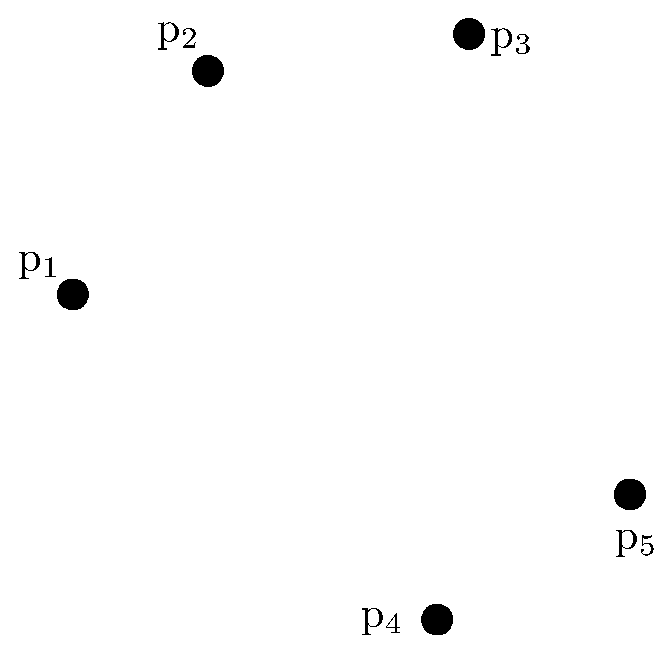
\includegraphics[width=4cm]{Ncut5points.eps}}
\put(6,0.8){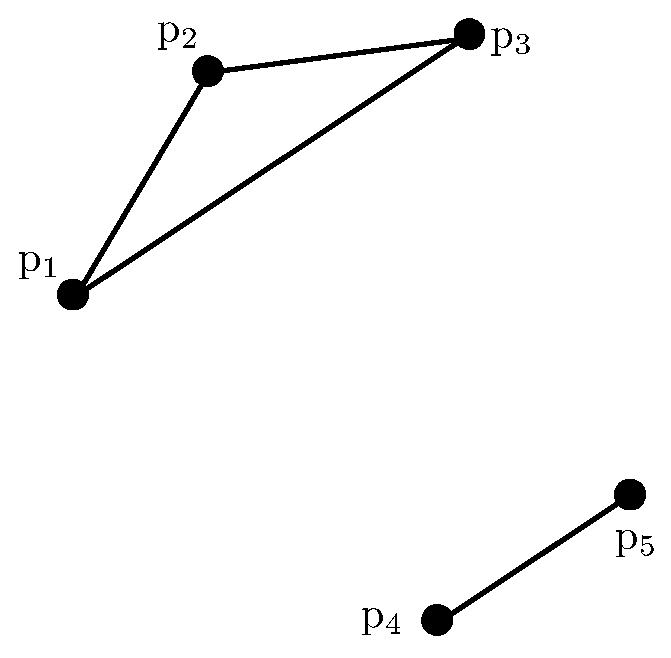
\includegraphics[width=4cm]{Ncut5discon.eps}}
\put(12,0.8){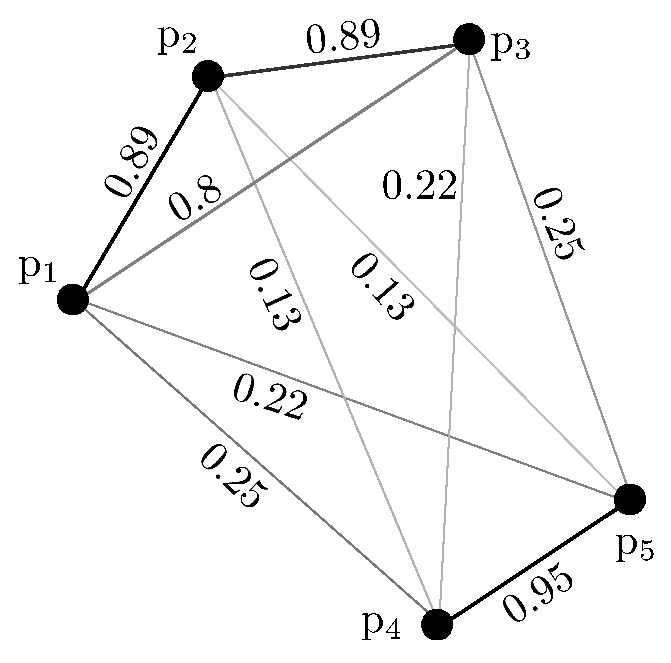
\includegraphics[width=4cm]{Ncut5simgra.eps}}
\put(2,0){(a)}
\put(8,0){(b)}
\put(14,0){(c)}
\end{picture}%}
 \caption{グラフの解析によるクラスタリング.グラフの節と枝はそれぞれ
データとデータ間の関係の深さを表す.
(a)与えられたデータ点.(b)クラスタを表す非連結グラフ.
(c)枝がデータ間の類似度を持っている類似度グラフ.}
\label{fig:Ncut5}
\end{center}
\end{figure}


データ集合が与えられたとき,
グラフを使って自動的にクラスタを見つけられるだろうか?
例えば,図\ref{fig:Ncut5}(a)のように,
5つのデータ点が与えられたときに2つのクラスタを見つけたいとする.
任意のデータ点の間のつながり(隣接)が分かっているならば,
図\ref{fig:Ncut5}(b)のようなグラフを作ることができる.
図の例では,他と連結していない2つのグラフの部分(連結成分)
によってグラフが構成されており,
2つのクラスタ$C_1=\{p_1,p_2,p_3\}$と$C_2=\{p_4,p_5\}$を特定できる.
このように,クラスタを表す連結成分を「計算」によって見つけることが,
グラフを用いたクラスタリングの目標である.

%How can we know the connectivity? % and compute the eigenvectors to obtain the clusters?
実際の応用では,データ間の隣接が明示的には与えられないかもしれないが,
データが持つ属性や特徴を使ってデータどうしの類似性か非類似性を
見積もれることがある(データ点の間の距離や内積など).
そのような場合は,例えば図\ref{fig:Ncut5}(c)のような
{\bf 類似度グラフ}(similarity graph)を作れる.
類似度グラフは,データ間の類似度を枝の重みとして与えた
単純グラフ\footnote{%
閉路も多重の枝も持たない無向グラフを単純グラフと呼ぶ.}である.
この類似度グラフの枝を切断して非連結のグラフにすることが
クラスタリングであると解釈できる.
その際,切断する枝の重みの和が最小になるように切断すべきである.




\Section{代数的なグラフの取り扱い}

\paragraph{隣接行列}
グラフを解析するため,{\bf 隣接行列}(adjacency matrix)を用いて
グラフを代数的に表すことができる.
$n$個の節を持つグラフ$G$の隣接行列$\mtr A$は,
節$i$から節$j$への枝の本数を第$i$行$j$列要素に持つ
$n\times n$行列である.
単純グラフは${0,1}$の2値の要素を持つ隣接行列で表される.
例えば,図\ref{fig:Ncut5}(b)の単純グラフの隣接行列は次のように書ける.
\begin{equation}
\mtr A=\smatrix{\normalsize}{ccccc}
{
0 & 1 & 1 & 0 & 0\\
1 & 0 & 1 & 0 & 0\\
1 & 1 & 0 & 0 & 0\\
0 & 0 & 0 & 0 & 1\\
0 & 0 & 0 & 1 & 0}
\end{equation}

\paragraph{次数行列}

節$i$から他の節への枝の本数を{\bf 次数}(degree)という.
隣接行列の第$i$行の行和は節$i$の次数に等しい.
$n$個の成分がすべて1のベクトルを$\vec 1_n$とすると,
$n$個の節の次数を成分に持つベクトルは
$\vec d=\mtr A\vec 1_n$のように計算できる.
次数を対角要素とする行列を{\bf 次数行列}(degree matrix)と定義する.
つまり,次数ベクトル$\vec d$を用いて$\mtr D=\diag(\vec d)$と書き表す.
図\ref{fig:Ncut5}(b)の単純グラフの次数ベクトルと次数行列は次のように書ける.
\begin{equation}
 \vec d=\mtr A\vec 1_n
=\smatrix{\small}{ccccc}
{
0 & 1 & 1 & 0 & 0\\
1 & 0 & 1 & 0 & 0\\
1 & 1 & 0 & 0 & 0\\
0 & 0 & 0 & 0 & 1\\
0 & 0 & 0 & 1 & 0}
\smatrix{\small}{c}{1\\ 1\\ 1\\ 1\\ 1}
=\smatrix{\small}{c}{2\\ 2\\ 2\\ 1\\ 1},
\quad \mbox{ }\quad
\mtr D=\diag\left(
\smatrix{\small}{c}{2\\ 2\\ 2\\ 1\\ 1}
\right)
=\smatrix{\small}{ccccc}
{
2 & 0 & 0 & 0 & 0\\
0 & 2 & 0 & 0 & 0\\
0 & 0 & 2 & 0 & 0\\
0 & 0 & 0 & 1 & 0\\
0 & 0 & 0 & 0 & 1}
\end{equation}


\paragraph{クラスタを表すベクトル}
$n$個のデータ点について,
成分がクラスタへの所属を表しているような$n$次元ベクトルを
{\bf クラスタ指示ベクトル}(cluster indicator)と呼ぶ.
図\ref{fig:Ncut5}のようなクラスタ$C_1=\{p_1,p_2,p_3\}$と$C_2=\{p_4,p_5\}$の
クラスタ指示ベクトルは,
それぞれ$\vec h^{(1)}=[1,1,1,0,0]$と$\vec h^{(2)}=[0,0,0,1,1]$である.

隣接行列$\mtr A$または次数行列$\mtr D$をクラスタ指示ベクトルに乗ずると,
クラスタに属す節の次数の総和が得られる.例えば,
\begin{equation}
\mtr A\vec h^{(1)}
=\smatrix{\small}{ccccc}
{
0 & 1 & 1 & 0 & 0\\
1 & 0 & 1 & 0 & 0\\
1 & 1 & 0 & 0 & 0\\
0 & 0 & 0 & 0 & 1\\
0 & 0 & 0 & 1 & 0}
\smatrix{\small}{c}{1\\ 1\\ 1\\ 0\\ 0}
=\smatrix{\small}{c}{2\\ 2\\ 2\\ 0\\ 0}
\quad \mbox{または}\quad
\mtr D\vec h^{(1)}
=\smatrix{\small}{ccccc}
{
2 & 0 & 0 & 0 & 0\\
0 & 2 & 0 & 0 & 0\\
0 & 0 & 2 & 0 & 0\\
0 & 0 & 0 & 1 & 0\\
0 & 0 & 0 & 0 & 1}
\smatrix{\small}{c}{1\\ 1\\ 1\\ 0\\ 0}
=\smatrix{\small}{c}{2\\ 2\\ 2\\ 0\\ 0}
\label{eq:counting degrees}
\end{equation}



\paragraph{ラプラシアン行列}
% variants
グラフ理論では,
グラフの{\bf ラプラシアン行列}(Laplacian matrix)が
$\mtr L=\mtr D-\mtr A$と定義されている.
{\bf ラプラシアン}とは,任意の点における値と
その近傍の平均値の差を測る2階微分演算子のことである.
もし,グラフの節を定義域として何らかの関数$f$が定義されていたら,
$\mtr L$はグラフ上で$f$のラプラシアンを計算する演算子になる.
例えば,図\ref{fig:Ncut5}(b)のグラフのラプラシアン行列$\mtr L$を
グラフ上の関数$f$に作用させると,
\begin{equation}
\mtr L
=\smatrix{\small}{ccccc}
{
2 & -1 & -1 & 0 & 0\\
-1 & 2 & -1 & 0 & 0\\
-1 & -1 & 2 & 0 & 0\\
0 & 0 & 0 & 1 & -1\\
0 & 0 & 0 & -1 & 1}
\quad \mbox{, }\quad
\mtr L\vec f=
\mtr L
\smatrix{\small}{c}{f(p_1)\\ f(p_2)\\ f(p_3)\\ f(p_4)\\ p(p_5)}
=
\smatrix{\scriptsize}{c}{
2\left(f(p_1)-\frac{f(p_2)+f(p_3)}{2}\right)\\
2\left(f(p_2)-\frac{f(p_1)+f(p_3)}{2}\right)\\
2\left(f(p_3)-\frac{f(p_1)+f(p_2)}{2}\right)\\
f(p_4)-f(p_5)\\
f(p_5)-f(p_4)}.
\end{equation}
という計算になる.
$\mtr L\vec f$の第1成分は,
$p_1$における$f$と,
隣接する$p_2$および$p_3$における$f$の平均値との
差になっていることがわかる.


ラプラシアン行列にはいくつかの興味深い性質がある.
\begin{itemize}
\item
任意のグラフについて
$\mtr L\vec 1_n=\mtr D\vec 1_n-\mtr A\vec 1_n=\vec d-\vec d=0\vec 1_n$が
必ず成り立つので,
$\mtr L$は少なくともひとつゼロの固有値を持ち,
その固有ベクトルは$\vec h=\vec 1_n$である.
\item
グラフが$k$個の連結成分からなるとき,
連結成分を表すクラスタ指示ベクトル$\vec h^{(l)}$ ($l=1,\dots,k$)が
ラプラシアン行列$\mtr L$のゼロの固有値に属する固有ベクトルになる.
このことは簡単に確認できる.
クラスタ$C_l$について,式(\ref{eq:counting degrees})のように
$\mtr A\vec h^{(l)}=\mtr D\vec h^{(l)}$が成り立つから,
$\mtr L\vec h^{(l)}=(\mtr D-\mtr A)\vec h^{(l)}=0\vec h^{(l)}$を得る.
\item
一般に,$\mtr L$のゼロの固有値が$k$個ならば,
グラフの連結成分は$k$個ある(演習問題\ref{ex:k indicators}).
\item
ラプラシアン行列の固有値は非負である(演習問題\ref{ex:L has nonnegative eigs}).
ラプラシアン行列$\mtr L$の固有値は{\bf グラフスペクトル}
(graph spectra)と呼ばれる.
\end{itemize}
ひとつの連結成分からなるグラフのラプラシアン行列はゼロの固有値をひとつ持つ.
グラフが複数の連結成分からなるかどうかは第2固有値から判明する.
それゆえ,第2固有値は{\bf 代数的連結度}(algebraic connectivity)と呼ばれる.
また,第2固有値に属する固有ベクトルは
{\bf Fiedlerベクトル}(Fiedler vector)\cite{Fiedler73}とも呼ばれる.



\Section{グラフのスペクトルと分割}

\paragraph{グラフの連結成分を見つける}
クラスタ指示ベクトルは,ラプラシアン行列のゼロの固有値に属する
固有ベクトルである.
この性質を利用して,グラフの連結成分として
クラスタを見つけるアルゴリズムを\ref{alg:finding disconnected components}に示す.
このように,データの関係を表現するグラフを記述する行列の
固有値解析によってクラスタを見つけることができる.


\begin{algorithm}[t]
\caption{連結成分を見つけるクラスタリング}
\label{alg:finding disconnected components}
\begin{algorithmic}[1]
\REQUIRE
隣接行列$\mtr A$;
\ENSURE クラスタの集合$\mathcal{C}=\{ C_1,\dots,C_k \}$;
\STATE
次数行列$\mtr D=\diag(\mtr A\vec 1_n)$を計算する;
\STATE
ラプラシアン行列$\mtr L=\mtr D-\mtr A$を計算する;
\STATE
$\mtr L$のゼロ固有値に属する固有ベクトル$\vec h^{(l)}$を計算する;
\STATE
$h_i^{(l)}\neq 0$ならば$i$を$C_l$に所属させる.
\end{algorithmic}
\end{algorithm}





\paragraph{類似度グラフを分割する}

%The clustering task can then be interpreted as cutting the similarity graph
%into disconnected components so as to minimize the sum of the cut-edge weights.


%\paragraph{Affinity matrix}
類似度グラフの枝のうち小さな類似度を持つものを切断して
クラスタを作ることを考える.
データ間の関係が類似度グラフとして与えられたとき,これを
{\bf 類似度行列}(affinity/similarity matrix)によって
代数的に表すことができる.
類似度行列は隣接行列を実数に拡張したようなものである.
類似度行列$\mtr W$の第$i$行$j$列要素は
節$i$から節$j$への枝の重み(つまり類似度)である.
図\ref{fig:Ncut5}(c)の類似度グラフの類似度行列は次のように書ける.
\begin{equation}
 \mtr W=
\smatrix{\small}{ccccc}
{
0 & 0.89 & 0.80 & 0.25 & 0.22\\
0.89 & 0 & 0.89 & 0.13 & 0.13\\
0.80 & 0.89 & 0 & 0.22 & 0.25\\
0.25 & 0.13 & 0.22 & 0 & 0.95\\
0.22 & 0.13 & 0.25 & 0.95 & 0}
\end{equation}
%
類似度グラフの次数行列$\mtr D$とラプラシアン行列$\mtr L$も
同様に類似度行列を用いて定義される.
\begin{equation}
 \mtr D=\diag(\mtr W\vec 1_n)
\end{equation}
\begin{equation}
 \mtr L=\mtr D-\mtr W
\end{equation}

類似度グラフのどの節も非ゼロの重みの枝をひとつ以上持つならば,
類似度グラフには非連結成分がない.
その類似度グラフのラプラシアン行列はひとつだけゼロ固有値を持ち,
固有ベクトルは$\vec h=\vec 1_n$である.
たとえ類似度グラフが明らかに$k$個の部分グラフからなっていても,
それらは小さな重みの枝で弱く結ばれているので,
アルゴリズム\ref{alg:finding disconnected components}によって
クラスタ指示ベクトル$\vec h^{(l)}$は得られない.
その代わり,類似度グラフのラプラシアン行列は$k$個の小さな固有値を持ち,
それらの固有ベクトルがクラスタを教えてくれる.
なぜならば,固有ベクトルがクラスタ指示ベクトルの近似になっているからである.
$\mtr W\vec h^{(l)}\neq\mtr D\vec h^{(l)}$なので,
$\mtr L\vec h^{(l)}=(\mtr D-\mtr W)\vec h^{(l)}\neq 0\vec h^{(l)}$である.
しかし,$\mtr D\vec h^{(l)}$と$\mtr W\vec h^{(l)}$の差は,
第$l$部分グラフの節と他の部分グラフの節の間の枝が持つ
小さな重みの総和を成分とする小さなベクトルに過ぎない.


図\ref{fig:Ncut5}(c)の類似度グラフの場合,
ラプラシアン行列の固有値は0, 0.99, 2.50, 2.96, 3.01である.
明らかに小さな固有値がふたつ存在し,
それらに属する固有ベクトルを列に並べると
\begin{equation}
 \mtr H_2=[\vec h^{(1)}, \vec h^{(2)}]=
\smatrix{\small}{rr}
{
0.45 & 0.33\\
0.45 & 0.43\\
0.45 & 0.33\\
0.45 & -0.55\\
0.45 & -0.55}.
\end{equation}
という行列を作れる.
固有ベクトル$\vec h^{(1)}$と$\vec h^{(2)}$はクラスタ指示ベクトルそのものではない.
しかし,行列$\mtr H_2$の全5行を2次元空間の5点のデータと見なしてプロットすると,
図\ref{fig:Ncut5clsind}のように2箇所に固まってクラスタが形成されていることがわかる.
これらのクラスタは$k$平均クラスタリング($k$-means clustering)や閾値処理程度の
簡単なベクトル量子化\footnote{%
小数点以下を四捨五入するなど,実数を何種類かの整数(または記号)のひとつに
置き換えることを量子化という.
同様に,ベクトルを何種類かの整数(または記号)のひとつに対応させることを
ベクトル量子化と呼ぶ.
ベクトルで表されるデータのクラスタリングはベクトル量子化の一手法である.
}で特定することができる.


\begin{figure}[h]
\setlength{\unitlength}{1cm}
\begin{center}
%\fbox{
\begin{picture}(6,5)
\put(0,0){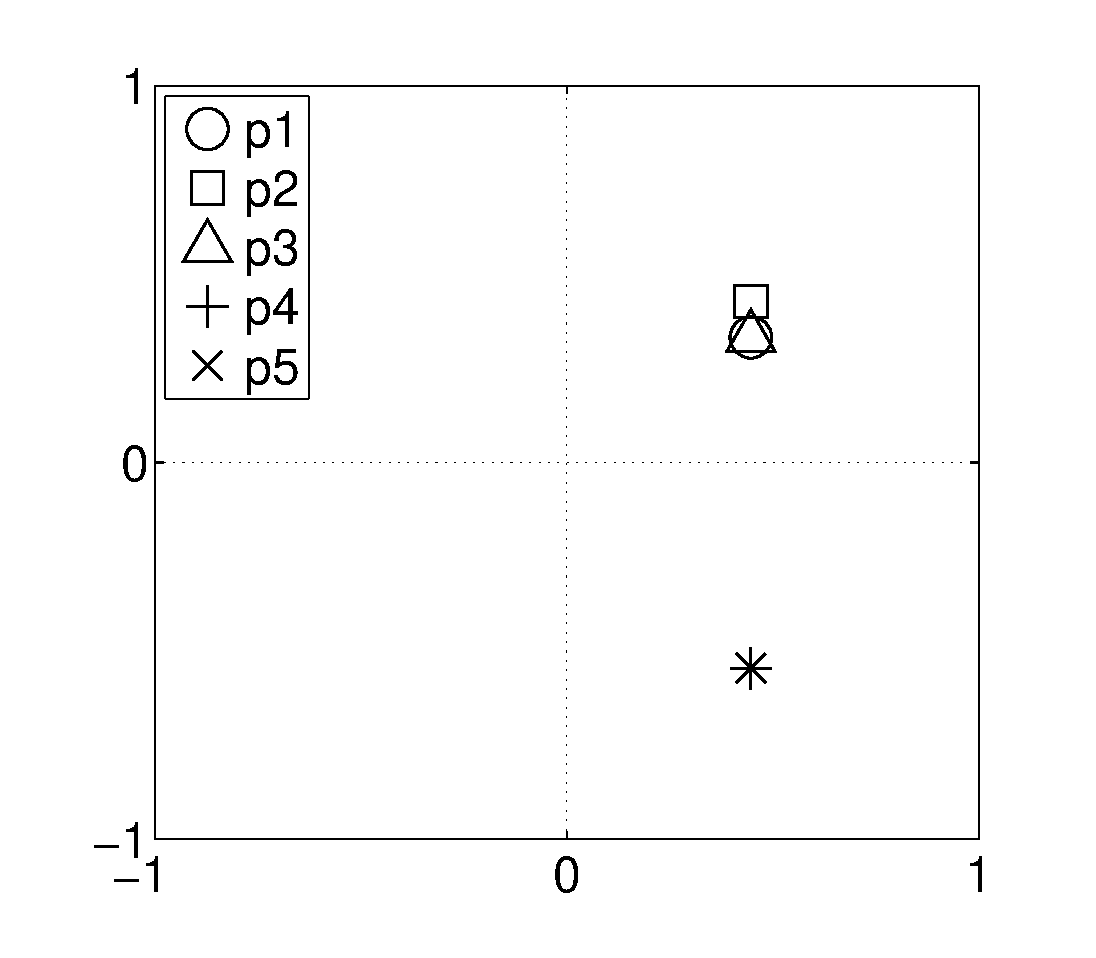
\includegraphics[width=6cm]{Ncut5clsind.eps}}
\end{picture}%}
 \caption{$\mtr H_2$の5行が2次元空間でふたつの密なクラスタを呈す.}
\label{fig:Ncut5clsind}
\end{center}
\end{figure}

このように,グラフを表す行列から固有ベクトルを計算すると,
類似度グラフの分割による$n$個のデータ点のクラスタリングは,
$k$次元空間の$n$個の点のクラスタリングに帰着する.


\Section{スペクトラルクラスタリングのアルゴリズム}

\begin{algorithm}[t]
\caption{スペクトラルクラスタリング}
\label{alg:spectral clustering}
\begin{algorithmic}[1]
\REQUIRE
類似度行列$\mtr W$, クラスタ数$k$;
\ENSURE クラスタの集合$\mathcal{C}=\{ C_1,\dots,C_k \}$;
\STATE
次数行列$\mtr D=\diag(\mtr W\vec 1_n)$を計算する;
\label{step:D}
\STATE
Rcut\cite{Hagen92}の場合: \\
ラプラシアン行列$\mtr L=\mtr D-\mtr W$の$k$個の小さな固有値に属する
固有ベクトルを列に並べた行列
$\mtr X_k=[\vec x^{(1)},\dots,\vec x^{(k)}]\in\mathbb{R}^{n\times k}$を作る;\\
Ncut\cite{Shi00,Yu03})の場合: \\
正規化類似度行列$\mtr S=\mtr D^{-1/2}\mtr W\mtr D^{-1/2}$の
$k$個の大きな固有値に属する
固有ベクトルを列に並べた行列
$\mtr X_k=[\vec x^{(1)},\dots,\vec x^{(k)}]\in\mathbb{R}^{n\times k}$を作る;
\label{step:eigen}
\STATE
$\mtr X_k$の各行ベクトルを正規化する;
\STATE
ベクトル量子化によって各データ点をクラスタのひとつ$C_l\in\mathcal{C}$に所属させる: 
典型的には,$\mtr X_k$の$n$本の行ベクトルに$k$平均クラスタリングを適用する.
\end{algorithmic}
\end{algorithm}

固有値解析に基づくデータクラスタリングを
アルゴリズム\ref{alg:spectral clustering}に示す.
このアルゴリズムは,グラフの$k$分割の「コスト」を最小化する問題について,
クラスタ指示ベクトルを離散2値から実数へ緩和することで導出される.
グラフを切断するコストは,クラスタの下記の性質を考慮して設計されている.
\begin{description}
\item[外的分離(external isolation)]
クラスタが互いに離れていること.
第$l$クラスタ$C_l$の全データ点と他のクラスタのデータ点をつなぐ枝の重みの和は,
${\vec h^{(l)}}^\top\mtr L\vec h^{(l)}$のように計算できる.この値は小さいほどよい.
$C_l$が他のクラスタから離れるほど小さくなるからである.
\item[内的結合(internal cohesion)]
クラスタ内のデータが互いに近いこと.
第$l$クラスタ$C_l$内のデータの個数は${\vec h^{(l)}}^\top\vec h^{(l)}$である.
$C_l$内のデータから他の節への枝の重みの総和は${\vec h^{(l)}}^\top\mtr D\vec h^{(l)}$
のように計算できる.
どのクラスタについても,これらの量が大きいほどよい.
各クラスタがよくまとまっていて,バランスがとれているほど大きくなるからである.
\end{description}

%There are some variants of spectral clustering.
スペクトラルクラスタリングのためのグラフ切断コストがいくつか設計されている.
\begin{eqnarray}
&\mbox{Ratio cut \cite{Hagen92}}:&
J\msub{Rcut}(\mtr H)=
\sum_{l=1}^k\frac{{\vec h^{(l)}}^\top\mtr L\vec h^{(l)}}{\vec {h^{(l)}}^\top\vec h^{(l)}}\label{eq:Rcut cost}\\
&\mbox{Normalized cut \cite{Shi00,Yu03}}:&
J\msub{Ncut}(\mtr H)=
\sum_{l=1}^k\frac{{\vec h^{(l)}}^\top\mtr L\vec h^{(l)}}{{\vec h^{(l)}}^\top\mtr D\vec h^{(l)}}\label{eq:Ncut cost}
%\\
%&\mbox{Min-max cut \cite{Shi00,Yu03}}:&
%J\msub{Mcut}(\mtr H)=
%\sum_{l=1}^k\frac{\vec h_l^\top\mtr L\vec h_l}{\vec h_l^\top\mtr W\vec h_l}
\end{eqnarray}
コスト$J\msub{Rcut}(\mtr H)$や$J\msub{Ncut}(\mtr H)$は,
$k$本のクラスタ指示ベクトル$\vec h^{(l)}$ ($l=1,\dots,k$)の関数である.
コストが最小になる$\mtr H=[\vec h^{(1)},\dots,\vec h^{(k)}]$を探す問題は
組合せ最適化問題である.
式(\ref{eq:Rcut cost})や式(\ref{eq:Ncut cost})を最小化する問題を
制約付き対角和最小問題に書き換え,
クラスタ指示ベクトル$\vec h^{(l)}$を
実ベクトル$\vec x^{(l)}\in\mathbb{R}^n$と見なすと近似的な解法が得られる.
実数のクラスタ指示ベクトル$\vec x^{(l)}$は次のような固有値問題の
固有ベクトルとして求まる.
\begin{eqnarray}
&\mbox{Ratio cut}:&
\mtr L\vec x^{(l)}=\lambda_l\vec x^{(l)}\\
&\mbox{Normalized cut}:&
\mtr S\vec x^{(l)}=\mu_l\vec x^{(l)}
%\mtr L\vec y_l=\lambda_l\mtr D\vec y_l,\quad \vec x_l=\mtr D^{1/2}\vec y_l\\
%&\mbox{Min-max cut}:&
\end{eqnarray}
ただし,$\lambda_l$ ($l=1,\dots,k$) は$\mtr L$の$k$個の小さな固有値,
$\mu_l$ ($l=1,\dots,k$) は$\mtr S=\mtr D^{-1/2}\mtr W\mtr D^{-1/2}$の
$k$個の大きな固有値である.
導出の詳細は文献\cite{Luxburg07}が詳しい.





\Section{演習問題}
\begin{enumerate}
\item
\label{ex:k indicators}
連結成分が$k$個あるグラフ$G$のラプラシアン行列を$\mtr L$とする.
$\mtr L$のゼロの固有値が$k$個ならば,$G$の連結成分は$k$個あることを証明せよ.\\
ヒント:
連結成分を表す$k$本のクラスタ指示ベクトル$\vec h^{(l)}$ ($l=1,\dots,k$)が
$\mtr L$の固有ベクトルであり,その固有値はゼロであることから,
$\mtr L$の固有値のうち少なくとも$k$個はゼロであると言える.
$\mtr L$のゼロの固有値に属する固有ベクトルは,
クラスタ指示ベクトルまたはその線形結合で表せるベクトルに
限られることを示せばよい.
\item
\label{ex:L has nonnegative eigs}
ラプラシアン行列の固有値は非負であることを証明せよ.\\
ヒント:
関数$q(\vec h)=\vec h^\top\mtr L\vec h$を,行列$\mtr L$の二次形式と呼ぶ.
$\|\vec h\|_2=1$の条件下で二次形式$q(\vec h)$の極値は$\mtr L$の固有値となる.
また,隣接行列$\mtr A$の要素を用いてラプラシアン行列$\mtr L=\mtr D-\mtr A$の
二次形式を書き表すと$q(\vec h)\geq 0$が示せる.
%ラプラシアン行列$\mtr L$は対称行列なので,固有ベクトルは互いに直交する.
%固有ベクトルを列に並べた行列を$\mtr H$とすると$\mtr H^\top=\mtr H$が成り立つ.
%$\mtr L=\mtr H\mtr{\mit\Lambda}\mtr H^\top$
%二次形式の
%対称行列の固有値
\item
スペクトラルクラスタリングを2次元の点集合
(例えば\href{http://cs.joensuu.fi/sipu/datasets/}{Clustering datasets\\ (http://cs.joensuu.fi/sipu/datasets/)}に適用せよ.
ただし,点$\vec p^{(i)}$と点$\vec p^{(j)}$ ($i\neq j$)の類似度$w_{ij}$を
次式のように定義する.
\begin{equation}
 w_{ij}=\exp\left(-\frac{\| \vec p^{(j)}-\vec p^{(i)} \|_2^2}{2\sigma^2}\right)
\end{equation}
$\sigma$は尺度のパラメタで,近いと見なす点間の距離の目安である.
例えば,下記のMATLABコードのようにデータ集合
\href{http://cs.joensuu.fi/sipu/datasets/spiral.txt}{Spiral}または
\href{http://cs.joensuu.fi/sipu/datasets/D31.txt}{D31}に試してみよ.
\lstset{language=Matlab}
\lstset{basicstyle={\tt},identifierstyle={\bfseries},keywordstyle={\bfseries}}
\lstset{tabsize=2,showstringspaces=false}
\lstset{commentstyle={\color[rgb]{0,0.5,0}}}
\lstset{flexiblecolumns=true}
\lstset{classoffset=1,breaklines=true,morecomment=[l]{//}}
%\lstset{columns=[l]{fullflexible}}
%\lstset{numbers=left,stepnumber=1,numberstyle={\scriptsize},numbersep=4ex}
\lstset{frame=tBlR,rulecolor={\color[gray]{0.75}},rulesepcolor={\color[gray]{0.75}}}
\lstset{framesep=2ex}
\lstset{xleftmargin=4ex,xrightmargin=4ex}
%\lstset{backgroundcolor={\color[rgb]{1,1,0.95}}}
\begin{lstlisting}
close all

% データ集合を読み込む.
data = load('spiral.txt');
n = size(data, 1);

% クラスタ数と尺度を設定する.
k = 3; sigma = 1.0;

% 類似度行列Wと正規化類似度行列Sを計算する.
pairdist = pdist(data(:,1:2));
W = exp(- squareform(pairdist.^2 / (2.0 * sigma.^2))) - eye(n, n);
Dinvsq = diag(1./sqrt(sum(W, 2)));
S = Dinvsq * W * Dinvsq;

% 固有ベクトルXと固有値Mを求める.
[X, M] = eig(S);
[M,idx] = sort(diag(M),'descend');
figure, plot(1:n, M)

% 上位k本の固有ベクトルを取り出して行を正規化する.
X = X(:, idx(1:k));
X = diag(1./sqrt(sum(X.^2, 2))) * X;

% k平均クラスタリングでベクトル量子化する.
c = kmeans(X, k, 'emptyaction', 'singleton');

% 結果を表示する.
marker10 = {'+', '*', 'x', '^', 'v', 's', 'p', '^', 'd', 'v'};
col = colormap(lines(16));
figure;
hold on
for t = 1:k,
    p = find(c == t);
    plot(data(p,1), data(p,2), marker10{mod(t,10)+1}, 'Color', col(mod(t,16)+1,:));
end
hold off
\end{lstlisting}
数千個のデータ点のクラスタリング
(数百万個以上の非ゼロ要素を持つ行列の固有ベクトル計算)
は数分かかるので注意せよ.


\item\yeeks
Webサイト
\href{http://www.cise.ufl.edu/research/sparse/matrices/}{the University of Florida Sparse Matrix Collection\\ (http://www.cise.ufl.edu/research/sparse/matrices/)}\\
を見て,
ひとつ行列を選べ
(例えば,{\tt c-45.mat}, {\tt jazz.mat}, {\tt wiki-Vote.mat}, {\tt netscience.mat}など).
その行列は無向グラフまたは2部グラフの類似度行列と見なせる.
スペクトラルクラスタリングを適用せよ.
固有値をプロットしてクラスタ数を推測せよ.
できればグラフのクラスタを可視化せよ.\\
ヒント:Ncutを適用するサンプルコードは下記のとおりである.
\begin{lstlisting}
close all
load('jazz.mat'); k = 4;
W = abs(Problem.A);
[m, n] = size(W);
Dinvsq1 = spdiags(1./sqrt(sum(W, 1)'), 0, n, n);
Dinvsq2 = spdiags(1./sqrt(sum(W, 2)), 0, m, m);
S = Dinvsq2 * W * Dinvsq1;

% スパース行列の特異値分解によって上位20*k個の固有値,固有ベクトルを計算する.
[X, M,~] = svds(S,20*k);
M = diag(M);
figure,plot(1:length(M), M, 'o')

X = X(:,1:k);
X = spdiags(1./sqrt(sum(X.^2, 2)), 0, m, m) * X;
c = kmeans(X, k, 'emptyaction', 'singleton');
\end{lstlisting}
\end{enumerate}





{\footnotesize
\bibliography{mybib_cls}
}




%\bibliographystyle{ieeetr}
%\bibliographystyle{splncs}
%\bibliographystyle{elsart-harv}
%\bibliographystyle{ipsjunsrt-e}
\bibliographystyle{ieicetr}




\Chapter{2部グラフで同時に分類 --- 共クラスタリングと特異値分解 ---}



\paragraph{前回と今回のあらすじ}
データを節,データ間のつながり(隣接)を枝で表したグラフを調べると,
データのグループ(クラスタ)を見つけることができる.
隣接の代わりにデータ間の類似度がわかる場合は,
枝に類似度が付された類似度グラフを分割することでデータをグループ分けできる.
なるべく小さな類似度が付された枝のみを切断してグラフを分割する問題は,
グラフを表す行列の固有値問題に近似して解ける.
この方法はスペクトラルクラスタリングと呼ばれている.

もし類似度グラフが2部グラフになる場合はどうだろうか.
集合が2つに分かれていて,
2つの集合の要素間にだけ対応または関連性が与えられている場合がそうである.
そのような場合は,対応または関連性に基づき2つの集合を
同時にクラスタリングできる.
その際,固有値問題は特異値分解と呼ばれる長方形の行列の分解に帰着する.


\Section{対応が表すデータのクラスタ}
%\section*{Data clusters indicated by correspondences}

ふたつのデータの集合があって,
一方の集合の要素(データ)が
もう一方の集合の部分集合に対応付けられている
と見なせるものがある.
単語(検索キーワード)と文書(Webページ)の対応や,
顧客と商品の対応などがそうである.
ふたつの集合の間に{\bf 対応}(correspondence)が与えられたとき,
その対応次第で,ふたつの集合を同時にグループ分けできることがある.

図\ref{fig:Bi_5x4}(a)は,
5種類の商品□と4人の顧客○の対応を表すグラフである.
どの商品も顧客の部分集合に対応付けられている.
例えば,商品5は顧客2と顧客4に買われている.
よく見ると,商品2も同様に顧客2と顧客4に買われている.
図\ref{fig:Bi_5x4}(b)のように少し並べ替えてみるとわかりやすい.
商品間や顧客間のつながりは与えられていないが,対応に基づき,
商品は$\{1,3,4\}$と$\{2,5\}$のグループに,
顧客は$\{1,3\}$と$\{2,4\}$のグループにそれぞれ分かれている.
このグループ分けは非常に有用である.
商品1を買う顧客は商品3や4も買う実態が明らかであり,
顧客1が買った商品を顧客3にお勧めする商法が有効であることもわかる.
類似の商品を顧客に提示することを{\bf コンテンツベースフィルタリング}(content-based filtering),
顧客の嗜好の類似性に基づき商品を提示することを{\bf 協調フィルタリング}(collaborative filtering)と呼ぶ.
%business method

\begin{figure}
\setlength{\unitlength}{1cm}
\begin{center}
%\fbox{
\begin{picture}(16,5.2)
\put(0,0.8){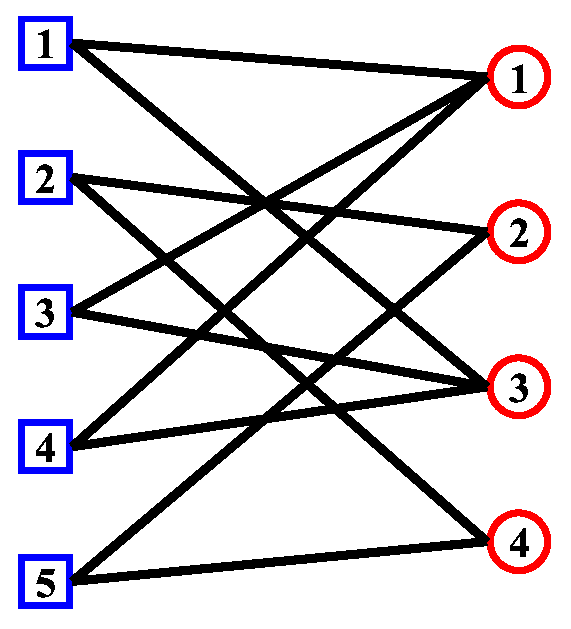
\includegraphics[width=4cm]{Bi_5x4A.eps}}
\put(6,0.8){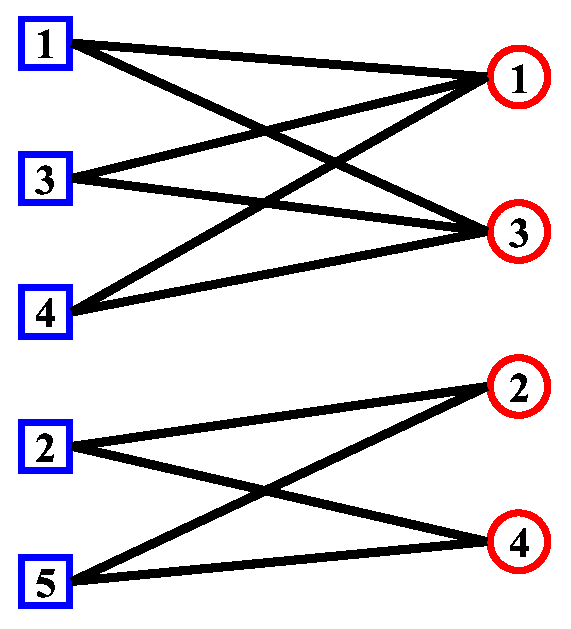
\includegraphics[width=4cm]{Bi_5x4As.eps}}
\put(12,0.8){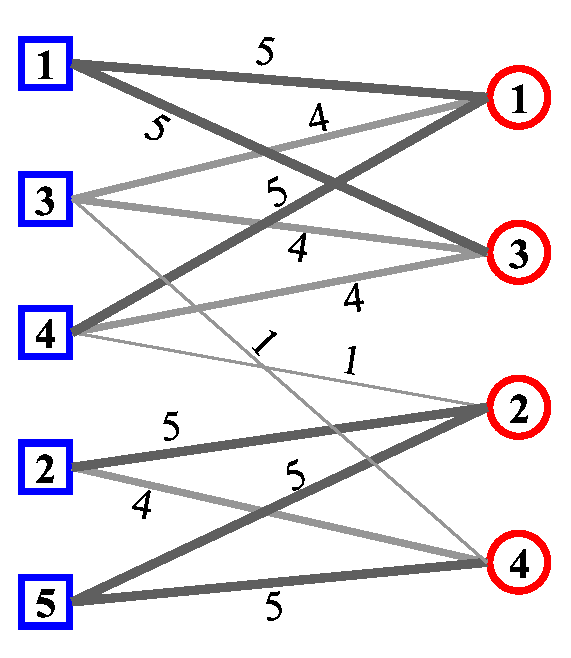
\includegraphics[width=4cm]{Bi_5x4Ws.eps}}
\put(1.8,0){(a)}
\put(7.8,0){(b)}
\put(13.8,0){(c)}
\end{picture}%}
 \caption{対応を表す2部グラフとクラスタリング.
5個の□と4個の○はそれぞれ商品と顧客を表す節である.
(a)商品とそれを買った顧客の対応を枝で表す2部グラフ.
(b) (a)の商品と顧客を並べ替えたもの.
(c)商品と顧客の関連性の強さ(購入数や評価点数など)を
重みとした類似度グラフ.}
\label{fig:Bi_5x4}
\end{center}
\end{figure}



\Section{2部グラフの切断によるデータの同時分類}

{\bf 2部グラフ}(bipartite graph)とは,節がふたつの集合に分かれていて,
一方の集合$M$の節ともう一方の集合$N$の節の間にだけ枝があるようなグラフである.
図\ref{fig:Bi_5x4}のように,
2部グラフは{\bf 対応}(correspondence)を表しており,
その対応次第で,ふたつの集合$M$と$N$の要素を
それぞれ同時にグループ分けできることがある.
そのようなグループ分けは{\bf 共クラスタリング}
(biclustering)%
\footnote{a.k.a. block clustering, co-clustering, or two-mode clustering.}
と呼ばれる.

実際の応用では,要素間の対応の有無ではなく,
関連性の強さで対応が表されていることがある.
例えば,表\ref{tab:stars}のように,
顧客が購入した商品の数や与えた星の数などを参考に,
商品と顧客の関係を調べることになるであろう.
そのような場合は,図\ref{fig:Bi_5x4}(c)のような
{\bf 2部類似度グラフ}(bipartite similarity graph)を作れる.
2部類似度グラフは,集合$M$の要素と集合$N$の要素の
対応を表す枝に重みが与えられている2部グラフである.
なるべく小さな重みの枝を切断して2部類似度グラフを非連結のグラフに
分割することが共クラスタリングであると解釈できる.


\begin{table}[h]
\begin{center}
\caption{関連性の強さで表された対応の例.
顧客と商品の対応を示す値が与えられている.実際の応用では,
顧客が商品を評価した点数かもしれなし,購入数かもしれない.}
\label{tab:stars}
\vspace{\baselineskip}
\begin{tabular}{l|cccc}
        & 顧客1 & 顧客2 & 顧客3 & 顧客4\\
\hline
商品1  & 5 & 0 & 5 & 0 \\
商品2  & 0 & 5 & 0 & 4 \\
商品3  & 4 & 0 & 4 & 1 \\
商品4  & 5 & 1 & 4 & 0 \\
商品5  & 0 & 5 & 0 & 5
\end{tabular}
\end{center}
\end{table}



\Section{2部グラフのスペクトラルクラスタリング}

集合$M$と$N$の要素間の対応を表す$m$対$n$の2部類似度グラフが与えられたとき,
集合$M$と$N$のそれぞれ$k$個のグループに分ける共クラスタリングを実行しよう.
Ncut\cite{Shi00,Yu03})のスペクトラルクラスタリングを
2部類似度グラフに適用すると,次のような計算手順になる.
\begin{enumerate}
\item
与えれれた2部類似度グラフを類似度行列$\mtr W$で表す.
\item
次数行列$\mtr D=\diag(\mtr W\vec 1_{m+n})$を作る.
\item
正規化類似度行列$\mtr S=\mtr D^{-1/2}\mtr W\mtr D^{-1/2}$を作る.
\item
$\mtr S$の$k$個の大きな固有値に属する固有ベクトルを計算し,
固有ベクトルを列に並べた行列
$\mtr X_k=[\vec x^{(1)},\dots,\vec x^{(k)}]\in\mathbb{R}^{(m+n)\times k}$を作る.
\item
$\mtr X_k$の各行を正規化し,ベクトル量子化する.
\end{enumerate}
この手順を更に詳しく見てみよう.


\paragraph{類似度行列の作成}
類似度行列$\mtr W$の第$i$行$j$列要素は第$i$節から第$j$節への
枝の重みである.
$m$対$n$の2部類似度グラフは$m+n$個の節を持つので,
$m+n$次正方の類似度行列で表せる.
$n$個の節を第$m+1,\dots,m+n$節とすると,
$(i,j)\in\{1,\dots,m\}\times\{m+1,\dots,m+n\}$のときだけ
類似度行列の要素$w_{ij}\defas c_{ij}$は非ゼロになり得る.
%ただし,$m$個の節の間に枝は無く,$n$個の節の間にも枝はないので,
%$(i,j)\in\{1,\dots,m\}^2\cup\{m+1,\dots,m+n\}^2$のとき
%隣接行列の要素は$a_{ij}=0$である.
\begin{equation}
\mtr W=\bmatrix{cc}{\mtr O & \mtr C\\ \mtr C^\top & \mtr O}
\label{eq:bipartite affinity matrix}
\end{equation}
類似度行列のブロック行列$\mtr C\in\mathbb{R}^{m\times n}$を
本書では{\bf 長方類似度行列}(rectangular similarity matrix)と呼ぶことにする.
\begin{description}
\item[例:]
図\ref{fig:Bi_5x4}(c)は$m=5$対$n=4$の2部類似度グラフであり,
$m+n=9$個の節を持つ.
商品1から5,顧客1から4を,それぞれ
第1から5節,第6から9節とすると,類似度行列は次のように書ける.
\begin{equation}
\mtr W=\smatrix{\normalsize}{ccccc|cccc}
{
0 & 0 & 0 & 0 & 0  &  5 & 0 & 5 & 0\\
0 & 0 & 0 & 0 & 0  &  0 & 5 & 0 & 4\\
0 & 0 & 0 & 0 & 0  &  4 & 0 & 4 & 1\\
0 & 0 & 0 & 0 & 0  &  5 & 1 & 4 & 0\\
0 & 0 & 0 & 0 & 0  &  0 & 5 & 0 & 5\\
\hline
5 & 0 & 4 & 5 & 0  &  0 & 0 & 0 & 0\\
0 & 5 & 0 & 1 & 5  &  0 & 0 & 0 & 0\\
5 & 0 & 4 & 4 & 0  &  0 & 0 & 0 & 0\\
0 & 4 & 1 & 0 & 5  &  0 & 0 & 0 & 0}
=\bmatrix{cc}{\mtr O & \mtr C\\ \mtr C^\top & \mtr O}
%\end{equation}
\qquad\mbox{ただし,}\quad
\mtr C=\smatrix{\normalsize}{cccc}
{
5 & 0 & 5 & 0\\
0 & 5 & 0 & 4\\
4 & 0 & 4 & 1\\
5 & 1 & 4 & 0\\
0 & 5 & 0 & 5}
\label{eq:bipartite affinity matrix 5x4}
\end{equation}
このように,2部類似度グラフの類似度行列$\mtr W$は,
対角ブロックにゼロ行列,
非対角ブロックに$\mtr C$と$\mtr C^\top$を持つ.
この長方類似度行列$\mtr C$は表\ref{tab:stars}そのものである.
\end{description}

%Ncut\cite{Shi00,Yu03})のスペクトラルクラスタリングでは,
%正規化類似度行列$\mtr S=\mtr D^{-1/2}\mtr W\mtr D^{-1/2}$の
%$k$個の大きな固有値に属する固有ベクトルを列に並べた行列
%$\mtr X_k=[\vec x_1,\dots,\vec x_k]\in\mathbb{R}^{n\times k}$から
%$k$個のクラスタを求める.
%ここで,

\paragraph{次数行列の作成}
$\mtr D=\diag(\mtr W\vec 1_{m+n})$は$\mtr W$の
行和
\begin{equation}
d_{i}=\sum_{j=1}^{m+n}w_{ij}=\left\{
\begin{array}{cll}
\displaystyle\sum_{j=1}^n c_{ij} & \mbox{if $1\leq i\leq m$} & \mbox{($\mtr C$の行和$\mtr C\vec 1_n$)}\\
\displaystyle\sum_{j=1}^m c_{ji} & \mbox{if $m+1\leq i\leq m+n$} & \mbox{($\mtr C$の列和$\mtr C^\top\vec 1_m$)}
\end{array}
\right.
\label{eq:degrees}
\end{equation}
からなる対角行列である.
また,$\mtr D^{-1/2}$も$1/\sqrt{d_i}$からなる対角行列である.
\begin{description}
\item[例:]
式(\ref{eq:bipartite affinity matrix 5x4})の類似度行列から得られる
次数行列$\mtr D$の対角要素は
\begin{eqnarray*}
 \mtr W\vec 1_9&=&[5+5,5+4,4+4+1,5+1+4,5+5,\;\;5+4+5,5+1+5,5+4+4,4+1+5]^\top\\
&=&[10,9,9,10,10,\;14,11,13,10]^\top
\end{eqnarray*}
である.
% The first $m=5$ entries and the following $n=4$ entries are
% the row and column sums of $\mtr C$.
初めの$m=5$個の要素は$\mtr C$の行和,
残りの$n=4$個の要素は$\mtr C$の列和であることがわかる.
\end{description}
%その対角要素の平方根の逆数からなる$\mtr D^{-1/2}$も対角行列である.
%ゆえに,
\paragraph{正規化類似度行列の作成}
正規化類似度行列$\mtr S$の第$i$行$j$列要素は
\[
 s_{ij}=\frac{w_{ij}}{\sqrt{d_id_j}}
\]
であり,式(\ref{eq:bipartite affinity matrix})と同様に
対角ブロックにゼロ行列を持っている.
式(\ref{eq:degrees})のように,$d_{i}$は$\mtr C$の行和と列和からなるので,
正規化類似度行列$\mtr S$は次のように書ける.
\begin{equation}
 \mtr S=\bmatrix{cc}{\mtr O & \mtr Z\\ \mtr Z^\top & \mtr O}
%\end{equation}
\qquad\mbox{ただし,}\quad
\mtr Z=\mtr D_2^{-1/2}\mtr C\mtr D_1^{-1/2},\quad
\mtr D_2=\diag(\mtr C\vec 1_n),\quad
\mtr D_1=\diag(\mtr C^\top\vec 1_m)
\label{eq:normalized affinity matrix}
\end{equation}


\paragraph{固有ベクトルの計算}
式(\ref{eq:normalized affinity matrix})のように,
$\mtr S$はブロック状の$m+n$次正方行列なので,
$m+n$次元の固有ベクトルを持つ.
この固有ベクトルを,
$m$次元ベクトル$\vec u\in\mathbb{R}^m$と
$n$次元ベクトル$\vec v\in\mathbb{R}^n$の連結と見なして
$\vec x=[\vec u^\top\,\vec v^\top]^\top$と置くと,
\begin{eqnarray*}
 \mtr S\vec x&=&\lambda\vec x\\
\bmatrix{cc}{\mtr O & \mtr Z\\ \mtr Z^\top & \mtr O}
\bmatrix{c}{\vec u\\ \vec v}
&=&
\bmatrix{c}{\lambda\vec u\\ \lambda\vec v}
\end{eqnarray*}
\begin{equation}
\therefore\quad
\mtr Z\vec v=\lambda\vec u,\qquad
\mtr Z^\top\vec u=\lambda\vec v
\label{eq:two eigen}
\end{equation}
$\vec u$または$\vec v$を消去すると,次式を得る.
\begin{equation}
 \mtr Z\mtr Z^\top\vec u=\lambda^2\vec u,\quad
\mtr Z^\top\mtr Z\vec v=\lambda^2\vec v
\label{eq:uv}
\end{equation}
%ただし,$\kappa=\lambda^2$である.
すなわち,
$\mtr S$の固有ベクトル$\vec x$を構成する
$\vec u$および$\vec v$は,それぞれ対称行列
$\mtr Z\mtr Z^\top\in\mathbb{R}^{m\times m}$および
$\mtr Z^\top\mtr Z\in\mathbb{R}^{n\times n}$の
固有ベクトルに他ならない.



\paragraph{ふたつの集合のクラスタリング}

$\mtr S$の$k$個の大きな固有値に属する
固有ベクトル$\vec x^{(1)},\dots,\vec x^{(k)}$を列に並べて,
行列$\mtr X_k=[\vec x^{(1)},\dots,\vec x^{(k)}]$を作成する.
行列$\mtr X_k$の全$m+n$行を$k$次元空間の$m+n$点と見なすと,
$k$箇所に固まってクラスタが形成されている.
これは,2部グラフの節のふたつの集合$M$と$N$の要素が
まとめて$k$個のクラスタに分類されたものである.
集合$M$の要素も$N$の要素も$k$個のクラスタに分けられており,
$M$のクラスタと$N$のクラスタの対応も知ることができる.

%2部グラフの一方の集合$M$をグループ分けするクラスタリングには,
%$\mtr X_k$の第1行から第$m$行までの部分行列を使う.
%同様に,集合$N$のクラスタリングには
%$\mtr X_k$の第$m+1$行から第$m+n$行までの部分行列を使う.

\begin{description}
\item[例:]
式(\ref{eq:bipartite affinity matrix 5x4}),(\ref{eq:normalized affinity matrix})
から得られる正規化類似度行列の固有値は
\[
1.00,\;0.92,\;0.12,\;0.03,\;0.00,\;-0.03,\;-0.12,\;-0.92,\;-1.00
\]
である.明らかに大きな固有値がふたつ存在し,
それらに属する固有ベクトルを列に並べると
\begin{equation}
\mtr X_2=[\vec x^{(1)},\vec x^{(2)}]=
\smatrix{\small}{rr}{
    0.32 &   0.31\\
    0.31 &  -0.38\\
    0.31 &   0.22\\
    0.32 &   0.24\\
    0.32 &  -0.40\\
    0.38 &   0.34\\
    0.34 &  -0.39\\
    0.37 &   0.33\\
    0.32 &  -0.36}
\quad\mbox{各行を正規化すると}\quad
\bar{\mtr X}_2
=\smatrix{\small}{rr}{
    0.72 &   0.69\\
    0.63 &  -0.78\\
    0.81 &   0.58\\
    0.80 &   0.59\\
    0.63 &  -0.78\\
    0.75 &   0.66\\
    0.66 &  -0.75\\
    0.75 &   0.66\\
    0.66 &  -0.75}
\end{equation}
という行列を作れる.
各行を$k=2$次元空間の点のデータと見なし,
第1行から第5行の$m=5$点を集合$M$の要素,
第6行から第9行の$n=4$点を集合$N$の要素としてプロットすると,
図\ref{fig:biNcut5vs4}のように2箇所に固まったクラスタが
形成されていることがわかる.
%ベクトル量子化して容易にクラスタを特定できる.
\end{description}
\begin{figure}[h]
\setlength{\unitlength}{1cm}
\begin{center}
%\fbox{
\begin{picture}(6,5)
\put(0,0){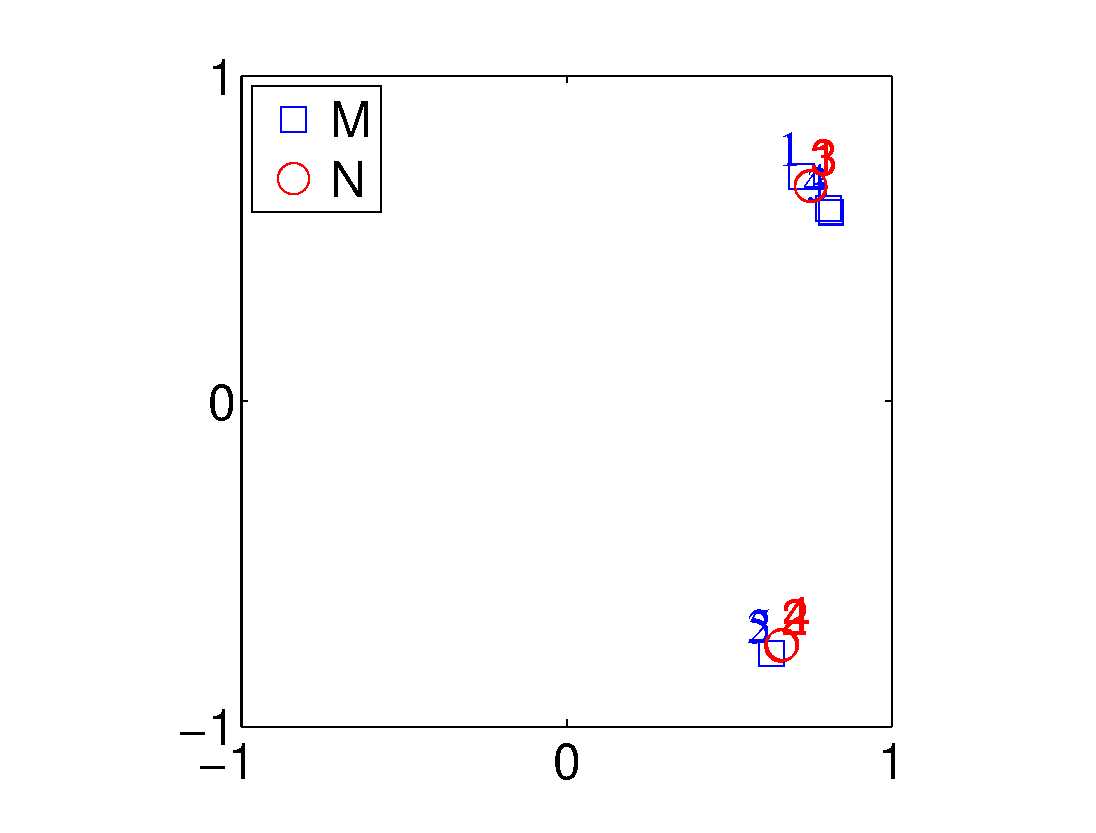
\includegraphics[width=6cm]{biNcut5vs4.eps}}
\end{picture}%}
 \caption{$\bar{\mtr X}_2$の5行が2次元空間でふたつの密なクラスタを呈す.
右上のクラスタは集合$M$の$\{1,3,4\}$と集合$N$の$\{1,3\}$からなる.
右下のクラスタは集合$M$の$\{2,5\}$と集合$N$の$\{2,4\}$からなる.
}
\label{fig:biNcut5vs4}
\end{center}
\end{figure}



\Section{特異値分解}

$\mtr Z$のランクを$r\defas\rank\mtr Z$とし,
%$\rank\mtr Z\mtr Z^\top=\rank\mtr Z^\top\mtr Z=r$が
%成り立つ(演習問題\ref{ex:rankZZ}).
%式(\ref{eq:uv})から,
%$r$個の非ゼロ固有値$\lambda_j^2$と
%これに属する$r$本の固有ベクトル$\vec u^{(j)}$と$\vec v^{(j)}$ ($j=1,\dots,r$)
%が存在する(演習問題\ref{ex:nonzero eigs}).
式(\ref{eq:uv})の非ゼロ固有値$\lambda_j^2$に属する
固有ベクトル$\vec u^{(j)}$と$\vec v^{(j)}$ ($j=1,\dots,r$)は
単位ベクトルであるとする.
対称行列の固有ベクトルは互いに直交するので,
\begin{equation}
\mtr U_r\defas[\vec u^{(1)},\dots,\vec u^{(r)}]\;\in\mathbb{R}^{m\times r}, \qquad
\mtr V_r\defas[\vec v^{(1)},\dots,\vec v^{(r)}]\;\in\mathbb{R}^{n\times r}
\label{eq:matrices of singular vectors}
\end{equation}
という行列を定義すると,
\begin{equation}
 \mtr U_r^\top\mtr U_r=\mtr V_r^\top\mtr V_r=\mtr I\in\mathbb{R}^{r\times r}
\label{eq:orthonormality}
\end{equation}
が成立する.
さらに,
固有値からなる対角行列を$\mtr K_r\defas\diag(\lambda_1,\dots,\lambda_r)$とすると,
式(\ref{eq:two eigen}),(\ref{eq:matrices of singular vectors}),(\ref{eq:orthonormality})から,
次式が導出される(演習問題\ref{ex:UZV}).
\begin{equation}
\mtr Z\mtr V_r=\mtr U_r\mtr K_r,\qquad
%\mtr Z^\top\mtr U=\mtr V\mtr K,\qquad
\therefore\quad
\mtr U_r^\top\mtr Z\mtr V_r=\mtr K_r
\label{eq:SVDr}
\end{equation}

%$\mtr U_r$と$\mtr V_r$はそれぞれ
%$m$次元実空間$\mathbb{R}^m$と
%$n$次元実空間$\mathbb{R}^n$における
%正規直交基底のうち$r$本の基底ベクトルであると見なせる.
$\mtr U_r$は$m$次元実空間$\mathbb{R}^m$の
正規直交基底のうち$r$本の基底ベクトルを並べた行列であると見なせる.
$\mtr V_r$についても同様である.
ゆえに,それぞれ残りの$m-r$本,$n-r$本の
基底ベクトルを追加した行列
$\mtr U\in\mathbb{R}^{m\times m}$と
$\mtr V\in\mathbb{R}^{n\times n}$を作成できる.
これら$\mtr U$と$\mtr V$は直交行列であり,
\begin{equation}
\mtr U^\top\mtr U=\mtr I\in\mathbb{R}^{m\times m},\qquad
\mtr V^\top\mtr V=\mtr I\in\mathbb{R}^{n\times n}
\label{eq:full orthonormality}
\end{equation}
を満たす.
ゆえに,
\begin{equation}
 \mtr Z=\mtr U\mtr K\mtr V^\top=\mtr U_r\mtr K_r\mtr V_r^\top
\label{eq:SVD}
\end{equation}
が成立する.
これは,行列$\mtr Z$の{\bf 特異値分解}(singular value decomposition; SVD)
と呼ばれている.
$\lambda_1,\dots,\lambda_r$は$\mtr Z$の特異値と呼ばれる.
また,$\vec u^{(1)},\dots,\vec u^{(r)}$と
$\vec v^{(1)},\dots,\vec v^{(r)}$は,それぞれ
$\mtr Z$の左特異ベクトル,右特異ベクトルと呼ばれる.




特異値分解を用いると,Ncutによる共クラスタリングは
アルゴリズム\ref{alg:biNcut}のような簡潔な手順になる.
\begin{algorithm}[t]
\caption{Ncutによる共クラスタリング}
\label{alg:biNcut}
\begin{algorithmic}[1]
\REQUIRE
クラスタ数$k$,\\
  $m$個の項目と$n$個の項目の間の関連性の強さを要素とする
長方類似度行列$\mtr C\in\mathbb{R}^{m\times n}$;
% relationships between pairwise items in two sets $M$ and $N$.
\ENSURE クラスタの集合$\mathcal{M}=\{ M_1,\dots,M_k \}$,$\mathcal{N}=\{ N_1,\dots,N_k \}$\\
  (ただし,$\sum_{l=1}^k|M_l|=m$,$\sum_{l=1}^k|N_l|=n$);
\STATE
行和と列和による次数行列$\mtr D_2=\diag(\mtr C\vec 1_n$と$\mtr D_1=\diag(\mtr C^\top\vec 1_m)$を計算する;
%\STATE
%正規化した長方類似度行列$\mtr Z=\mtr D_2^{-1/2}\mtr C\mtr D_1^{-1/2}$の
%$k$個の大きな特異値に属する左右の特異ベクトルを列に並べて,
%行列$\mtr U_k=[\vec u^{(1)},\dots,\vec u^{(k)}]\in\mathbb{R}^{m\times k}$と
%$\mtr V_k=[\vec v^{(1)},\dots,\vec v^{(k)}]\in\mathbb{R}^{n\times k}$を作る;
%\STATE
%$\mtr U_k$と$\mtr V_k$を結合して$\mtr X_k=\bmatrix{c}{\mtr U_k\\ \mtr V_k}\in\mathbb{R}^{(m+n)\times k}$を作る;
\STATE
正規化した長方類似度行列$\mtr Z=\mtr D_2^{-1/2}\mtr C\mtr D_1^{-1/2}$の
$k$個の大きな特異値に属する左右の特異ベクトル$\vec u^{(l)}$と$\vec v^{(l)}$ ($l=1,\dots,k$)を計算する;
\STATE
$\vec u^{(l)}$と$\vec v^{(l)}$を結合して
$\mtr X_k=\bmatrix{ccc}{\vec u^{(1)} & \cdots & \vec u^{(k)}\\ \vec v^{(1)} & \cdots & \vec v^{(k)}}\in\mathbb{R}^{(m+n)\times k}$を作る;
\STATE
$\mtr X_k$の各行ベクトルを正規化する;
\STATE
% quantize each row vector of $\mtr X_k$ into $k$ bins
$\mtr X_k$の各行を$k$個のビンにベクトル量子化して$\vec y\in[k]^{m+n}$を作る:
典型的には,$\mtr X_k$の$m+n$本の
行ベクトルを$k$平均クラスタリングする;
\STATE
$y_i=l$ ($i=1,\dots,m$) ならば項目$i$を$M_l$に所属させる.
\STATE
$y_{m+j}=l$ ($j=1,\dots,n$) ならば項目$j$を$N_l$に所属させる.
\end{algorithmic}
\end{algorithm}



\iffalse
まず,2部グラフの隣接行列から作ったラプラシアン行列の固有ベクトルが
クラスタ指示ベクトルになっていることを確認しよう.
$m$対$n$の2部グラフは$m+n$個の節を持ち,$m+n$次正方の隣接行列で表せる.
$n$個の節を第$m+1,\dots,m+n$節とすると,
$(i,j)\in\{1,\dots,m\}\times\{m+1,\dots,m+n\}$のときだけ
隣接行列の要素$a_{ij}\defas b_{ij}$は非ゼロになり得る.
%ただし,$m$個の節の間に枝は無く,$n$個の節の間にも枝はないので,
%$(i,j)\in\{1,\dots,m\}^2\cup\{m+1,\dots,m+n\}^2$のとき
%隣接行列の要素は$a_{ij}=0$である.
例えば,図\ref{fig:Bi_5x4}(a)は$m=5$対$n=4$の2部グラフであり,
$m+n=9$個の節を持つ.
商品1から5,顧客1から4を,それぞれ
節1から5,節6から9とすると,隣接行列は次のように書ける.
\begin{equation}
\mtr A=\smatrix{\normalsize}{ccccc|cccc}
{
0 & 0 & 0 & 0 & 0  &  1 & 0 & 1 & 0\\
0 & 0 & 0 & 0 & 0  &  0 & 1 & 0 & 1\\
0 & 0 & 0 & 0 & 0  &  1 & 0 & 1 & 0\\
0 & 0 & 0 & 0 & 0  &  1 & 0 & 1 & 0\\
0 & 0 & 0 & 0 & 0  &  0 & 1 & 0 & 1\\
\hline
1 & 0 & 1 & 1 & 0  &  0 & 0 & 0 & 0\\
0 & 1 & 0 & 0 & 1  &  0 & 0 & 0 & 0\\
1 & 0 & 1 & 1 & 0  &  0 & 0 & 0 & 0\\
0 & 1 & 0 & 0 & 1  &  0 & 0 & 0 & 0}
=\bmatrix{cc}{\mtr O & \mtr B\\ \mtr B^\top & \mtr O}
%\end{equation}
\qquad\mbox{ただし,}\quad
\mtr B=\smatrix{\normalsize}{cccc}
{
1 & 0 & 1 & 0\\
0 & 1 & 0 & 1\\
1 & 0 & 1 & 0\\
1 & 0 & 1 & 0\\
0 & 1 & 0 & 1}
\end{equation}
\fi




\Section{演習問題}
\begin{enumerate}
\item
\label{ex:UZV}
式(\ref{eq:SVDr})を導出せよ.
また,特異値分解の式(\ref{eq:SVD})を導出せよ.
\end{enumerate}




{\footnotesize
\bibliography{mybib_cls}
}





\end{document}
